\documentclass[12pt]{article}
%\usepackage[latin1]{inputenc}
\usepackage[T1]{fontenc}
\usepackage{geometry}
\usepackage{graphicx}
\usepackage{subcaption}
\usepackage[onehalfspacing]{setspace}
\usepackage{amsmath,amsfonts,amssymb,amsthm}
\usepackage{bm}
\usepackage{commath}
\usepackage{enumerate}
\usepackage{accents}
%\usepackage{enumitem}
\usepackage[shortlabels]{enumitem}
\usepackage{dsfont}
\usepackage{mathtools}
\usepackage{physics}
\usepackage{cite}
\usepackage[round]{natbib}
\usepackage{caption}
\captionsetup[figure]{font=small}
\usepackage{float}
%\usepackage{hyperref}
\usepackage{bbm}

\newtheorem*{theorem}{Theorem} 
\newtheorem*{lemma}{Lemma}
\newtheorem*{definition}{Definition}
\newtheorem*{corollary}{Corollary}
\newtheorem*{remark}{Remark}
\newtheorem*{example}{Example}
\newtheorem*{examples}{Examples}
\newcommand*{\QEDB}{\hfill\ensuremath{\square}}

\DeclareMathOperator*{\argmax}{arg\,max}
\DeclareMathOperator*{\argmin}{arg\,min}

\newcommand\independent{\protect\mathpalette{\protect\independenT}{\perp}}
\def\independenT#1#2{\mathrel{\rlap{$#1#2$}\mkern2mu{#1#2}}}

\interfootnotelinepenalty=10000
\allowdisplaybreaks
\geometry{
  left=2.5cm,
  right=2.5cm,
  top=2cm,
  bottom=2cm,
}

\begin{document}
\numberwithin{equation}{section}
\begin{titlepage}
	\centering
	{\scshape\LARGE Ludwig-Maximilians-Universit\"at M\"unchen \par}
	\vspace{1cm}
	{\scshape\Large Statistical Consulting Project \par}
	\vspace{1.5cm}
	{\huge\bfseries E-Complaints of Citizens and Responsiveness Strategies of Political Candidates and Parties: Investigating Large-Scale Unstructured Text  \par}	
	\vspace{0.8cm}	
	{\Large  Comparison of homepages of national and local political entities \par}
	\vspace{2cm}
	{\Large\itshape Simon Wiegrebe, Patrick Schulze \par}
	\vspace{2cm}	
	\begin{abstract}
		\begin{center}
		TBD
		\end{center}		
	\end{abstract}
	\vfill
	supervised by\par
	Prof. Dr. Christian Heumann and Prof. Dr. Paul W. Thurner

	\vfill

	{\large \today\par}
\end{titlepage}

\tableofcontents
\section{Introduction}
\label{Introduction}

The rise in popularity of social media has changed various aspects of private, public, and professional life over the last two decades. From a data-analytical point of view, this has led to an unprecedented increase in the supply of publicly available unstructured (text) data, ready to be analyzed. In fact, unstructured data makes up the lion's share of what is called \textit{big data} (\citealp{gandomi2015beyond}). At the same time, advances in the field of machine learning, particularly in \textit{Natural Language Processing} (NLP), have created numerous new opportunities for the analysis of such large-scale unstructured texts.

A field which has been particularly impacted by the use of social media (and the information extracted from it) is politics. At least since the 2016 Brexit vote and US presidential election, politicians have come to recognize not only that social media presence is ever more important, but also how strong a message their social media behavior can transmit. Among social media networks, Twitter is of particular importance, since it allows for direct communication between politicians and voters - and even more so after the Facebook-Cambridge Analytica data breach in 2018. As a consequence, there has been increasing academic interest in text-based (intra- and inter-)party politics (e.g., \citealp{ceron2017intra, daniel2019static, grimmer2010bayesian, quinlan2018show}). Moreover, unstructured text and the insights generated from it can subsequently be used as input for a broad variety of tasks, ranging from election forecasts (e.g., \citealp{burnap2016140, jungherr2016twitter, tumasjan2010predicting}) to prediction of stock market movements (e.g., \citealp{nisar2018twitter}).

A key challenge in analyzing large amounts of unstructured text is to reduce dimensionality and classify pieces of text: either into previously determined categories (for instance, sentiments), which corresponds to a supervised learning problem; or by trying to discover latent thematic clusters that govern the content of the documents, which is now an instance of unsupervised learning (since the number and labeling of clusters is to be determined). In this paper, we use a mixture of both strategies - an unsupervised \textit{topic model} followed by supervised regression analysis - and apply it to German politics. In particular, we construct a dataset where the text documents consist of Twitter messages by German Members of Parliament (MPs) and which furthermore contains a plenitude of personal MP-level data as well as socioeconomic data on an electoral-district level. Subsequently, we fit a \textit{Structural Topic Model} (STM) to the data to discover latent topics and analyze their relationship with document-level metadata. The focus of this paper lies on statistical and methodological aspects of topic models in general, but especially regarding the relation of topics to metadata, instead of specific (politological) hypothesis testing. Altogether, thus, the contribution of this paper is threefold: first, a broad and widely applicable dataset for future research, particularly in political science; second, a topic analysis of German parliamentarians' Twitter communication; and third, critical discussion of existing and development of new tools for (causal) inference within a topic modeling context.

We find that for most model specifications the majority of topics carry meaning, which can be regarded as a form of retrospective model validation. The fact that these topics are converted from mere word clusters into actually meaningful thematic clusters through manual labeling underlines the importance of human judgment in statistical topic modeling - this is in line with \cite{chang2009reading}, who show that solely focusing on quantitative metrics such as held-out likelihood does not guarantee meaningfulness of the latent space. As for document-level metadata, we discover some relevant associations between topic proportions and document features; particularly for the political parties, these relationships are in line with expectation. For continuous covariates such as unemployment and GDP the high degree of uncertainty induced by the underlying generative process of the STM renders relationships insignificant - though the observed tendencies are consistent across all modeling methodologies. The inclusion of a covariate to further model topical content (beyond its effect on topical prevalence) is found to reduce the meaningfulness of the latent space; furthermore, no natural candidate for the topical content variable exists in our case. Finally, we find that double usage of (prevalence) covariate information does not pose a problem, while double usage of document-level associations induces a substantial degree of overfitting.

The remainder of this paper is organized as follows. Section \ref{Theoretical Framework} provides the theoretical foundation of topic modeling, in particular the "component models" of the STM which we use for the major part of our analysis, as well as a brief discussion of inference and parameter estimation. Section \ref{Data} describes the data collection process, the data itself, and the data preprocessing necessary for topic modeling. Section \ref{Model Selection and Global Characteristics} discusses model selection, labeling as well as global characteristics of the latent space. In section \ref{Metadata Analysis - Topical Prevalence and Content}, we include document-level metadata into the analysis, presenting the corresponding theory and results. Section \ref{Overfitting and Causal Inference - Alternative Modeling Strategies} deals with alternative modeling approaches and strategies for causal inference. Finally, section \ref{Conclusion} concludes.
\section{Theoretical Framework}
\label{Theoretical Framework}

\subsection{Topic Modeling - Overview}
\label{Topic Modeling - Overview}

Topic models seek to discover latent thematic clusters, called topics, within a collection of discrete data, usually text; therefore, topic modeling can be regarded as dimensionality reduction technique. Furthermore, since both the number and content of topics is unknown beforehand (and can never be truly verified), topic modeling is an instance of unsupervised learning. Information retrieval (IR) research generally proposes the reduction of text documents to vectors of real numbers, each number representing (modified) counts of or terms. An instance of this proposed methodology is the \textit{tf-idf} scheme by \cite{salton1983information}, which for a collection of documents returns a term-by-document matrix where each row corresponds to a document in the corpus and the columns contain the respective \textit{tf-idf} term count. Since only words in a vocabulary of fixed length $V$ are considered, documents of unrestricted length are being reduced to vectors of a fixed length $V$. To further reduce dimensionality, the \textit{latent semantic indexing} (LSI) by \cite{deerwester1990indexing} applied singular value decomposition (SVD) to the \textit{tf-idf} document-term matrix. However, as \cite{blei2003latent} argue, the idea should be to develop a generative probabilistic model of text, in order to estimate to which extent the LSI methodology can align data with the generative text model; yet, given such a model, Bayesian methods or maximum likelihood estimation (MLE) would be much more direct, which is why the benefits of applying the LSI are not obvious. Picking up this shortcoming of LSI, \cite{hofmann1999probabilistic} introduced the \textit{probabilistic LSI} (pLSI) model. This generative data model allows for individual words to be sampled from a mixture model: they are drawn from a multinomial distribution, with latent random variables determining the mixture proportions, which in turn can be viewed as topics. However, the pLSI can only be regarded as partly probabilistic text model, since the mixing components themselves are fixed on a document level, thus lacking a probabilistic generating process.

In their \textit{Latent Dirichlet Allocation} (LDA) model, \cite{blei2003latent} included the generation of topic proportions into the generative probabilistic model, the resulting three-level hierarchical Bayesian mixture model marking the starting point of modern topic modeling. In order to present the main idea of LDA, we first introduce some notation and terminology that we will use throughout the remainder of this paper.

\begin{itemize}
\vspace{-0.25cm}
\item[•] A \textit{word} $w$ is the smallest unit of discrete text data. Words are instances of a vocabulary of $V$ unique \textit{terms} and can thus be indexed by $v \in \{1,\dots,V\}$. Mathematically, the $v$-th term in the vocabulary can be represented as a vector of length $V$, whose $v$-th component equals one, with all other components equalling zero. We will sometimes refer to the $v$-th term of the vocabulary simply as $v$. Words, along with document-level metadata, represent the actually observable data.
\vspace{-0.25cm}
\item[•] A \textit{document} $d \in \{1,\dots,D\}$ is a sequence of words of length $N_{d}$. For a given document $d$, we denote its words by $\boldsymbol{w}_d:=(w_{d,1},\dots,w_{d,N_{d}})$. Consequently, the $n$-th word of document $d$ is denoted by $w_{d,n}$.
\vspace{-0.25cm}
\item[•] A \textit{corpus} is a collection (or set) of $D$ documents. Therefore, $d \in \{1,\dots,D\}$ means that our corpus contains $D$ documents.
\vspace{-0.25cm}
\item[•] A \textit{topic} is a latent thematic cluster within a text corpus. The idea is that any collection of documents is made up of $K$ such topics, where the number of topics $K$ is an (unknown) hyperparameter which needs to be determined ex ante (see section \ref{Hyperparameter Search and Model Fitting} for hyperparameter determination in our specific use case). We will refer to topics simply by the actual \textit{topic index} (or \textit{topic number}) $k \in \{1,\dots,K\}$.
\vspace{-0.25cm}
\item[•] A \textit{topic-word distribution} $\boldsymbol{\beta}$ is a probability distribution over words, i.e., over the vocabulary. For a model containing $K$ topics (and no topical content variable, see section \ref{The Structural Topic Model} below), topic-word distributions do not vary across documents and uniquely characterize a topic: we denote the word distribution corresponding to the $k$-th topic by $\boldsymbol{\beta}_k$ and the matrix whose $k$-th column is topic $\boldsymbol{\beta}_k$ by $\boldsymbol{B}:=\boldsymbol{\beta}_{1:K}=[\boldsymbol{\beta}_1|\dots|\boldsymbol{\beta}_K]$. Each vector $\boldsymbol{\beta}_k$ thus has length $V$, while $B$ is a $V \times K$-matrix. Therefore, $k$ refers to the latent thematic cluster with topic index $k$ in general, and $\boldsymbol{\beta}_k$ refers to the underlying word distribution in particular.
\vspace{-0.25cm}
\item[•] A \textit{topic assignment} $\boldsymbol{z}_{d,n}$ is the assignment of the $n$-th word of document $d$ to a specific topic $k \in \{1,\dots,K\}$ (i.e., to the corresponding word distribution $\boldsymbol{\beta}_k$). Therefore, $\boldsymbol{z}_{d,n}$ is simply a vector of length $K$ whose $k$-th entry equals one and all other entries equal zero. This allows us to represent the word distribution corresponding to the $n$-th word in document $d$ as $\boldsymbol{\beta}_{d,n}:=B\boldsymbol{z}_{d,n}$ (again, for a model without topical content variable).
\vspace{-0.25cm}
\item[•] For a given document $d$, the corresponding \textit{topic proportions}, denoted by $\boldsymbol{\theta}_d$, are the proportions of the document's terms assigned to each of the topics $k \in \{1,\dots,K\}$. Topic proportions vary across documents. Since for each document $d$ the proportions of all $K$ topics must add up to one ($\sum_{k=1}^{K}\theta_{d,k}=1$, for all $d \in \{1,\dots,D\}$), topic proportions represent probabilities.
\vspace{-0.25cm}
\item[•] The \textit{bag-of-word} assumption is an assumption used in all (probabilistic) text models referenced in this paper, including LSI and pLSI, and states that only words themselves (and their counts) carry meaning, while word order or grammar do not. Statistically, this is equivalent to assuming that words within a document are \textit{exchangeable} (\citealp{aldous1985exchangeability}).

\end{itemize}

As mentioned above, LDA is the first generative probabilistic model of an entire text corpus. (Recall that pLSI is only probabilisitic for a fixed document.) 
Now, the generative process underlying LDA can be described as a two-step procedure, where for each document $d \in \{1,\dots,D\}$:

\begin{enumerate}[{1)}]
\vspace{-0.25cm}
\item Draw topic proportions $\boldsymbol{\theta}_d \sim \text{Dir}_K(\boldsymbol{\alpha})$.
\vspace{-0.25cm}
\item For each word $n \in \{1,\dots,N_d\}$:
	\begin{enumerate}[{a)}]
	\vspace{-0.25cm}    
    \item Draw a topic assignment $\boldsymbol{z_{d,n}} \sim \text{Multinomial}_K(\boldsymbol{\theta}_d)$.
	\vspace{-0.25cm}    
    \item Draw a word $w_{d,n} \sim \text{Multinomial}_V(\boldsymbol{\beta}_{d,n})$.
	\end{enumerate}
\end{enumerate}

\noindent
Thus, topic proportions are drawn from a Dirichlet distribution with $K$-dimensional $\boldsymbol{\alpha}$, with all components $\alpha_k > 0$, where the number of topics $K$ is a hyperparameter to be set by the user; the $\boldsymbol{\alpha}$-vector is estimated from the data. This means that for each document $d \in \{1,\dots,D\}$, the corresponding topic proportions $\boldsymbol{\theta}_d$ represent a $K$-dimensional vector which can take on values on the ($K-1$)-simplex, i.e., $\theta_{d,k} \geq 0, \sum_{k=1}^{K}\theta_{d,k}=1$. Also note that the Dirichlet distribution is the conjugate prior of the multinomial distribution, which greatly facilitates estimation (see section \ref{Inference and Parameter Estimation} on variational inference below). Put simply, for each document LDA first generates topic proportions, which are then used as weights for topic assignment. A word is then drawn from a topic-specific word distribution, which is determined by the topic assignment. These topic-specific word distributions $\boldsymbol{\beta}_k$ need to be estimated from data.
Note that LDA is a very simple, restrictive model in (at least) three ways:

\begin{enumerate}[label=(\roman*)]
\vspace{-0.25cm}
\item By using the Dirichlet distribution to generate topic proportions, potential correlations between topics cannot be captured due to the neutrality of the Dirichlet distribution.\footnote{Due to the constraint $\sum_{k=1}^{K}\theta_{k}=1$, there is clearly some degree of dependence between topic proportions. However, the dependence is minimal, as the Dirichlet distribution is characterized by complete neutrality: the components $\theta_1/(1-S_0), \theta_2/(1-S_1),\dots, \theta_K(1-S_{K-1})$ are mutually independent, where $S_0:=0$ and $S_k = \sum_{i=1}^{k}\theta_k, k \in \{1,\dots,K\}$. Stated differently, for each component $\theta_k, k \in \{1,\dots,K\}$, it holds that $\theta_k/(1-S_{k-1})$ is independent of the vector constructed by weighting all \textit{remaining} components by their total proportion (\citealp{james1980new})}. As a consequence, the occurrence of one topic within a document is not correlated with the occurrence of another topic (\citealp{blei2007correlated}). This is a restrictive simplification, as topics such as "sports" and "health" are much more likely to co-occur within a document than, say, "sports" and "war".
\vspace{-0.25cm}
\item Second, while topic proportions vary stochastically across documents, they do so given a single, global hyperparameter vector $\boldsymbol{\alpha}$; recalling the bag-of-words assumption, this implies that topic proportions are generated based merely on word counts (occurrences and co-occurrences), while additional document-level information is not taken into account. This is another unrealistic and limiting simplification, since researchers usually possess further document-specific information indicative of the topics addressed within the individual documents.
\vspace{-0.25cm}
\item Third, by construction, the topic-specific word distributions $\boldsymbol{\beta}_k$ are assumed to be identical for all documents. Similarly to the second restriction, this prevents researchers from using (document-level) information which might potentially influence the weighting of specific words within a topic.

\end{enumerate}

\noindent
Due to its simplicity and the resulting restrictions, the LDA has been used used as a building block for more advanced (and usually more specified) generative topic models. One model that builds on LDA, addressing some of its shortcomings, is the \textit{Correlated Topic Model} (CTM) by \cite{blei2007correlated}. Specifically, the CTM addresses the first one of the abovementioned restrictions: the inability to cope with inter-topic correlations. The model no longer uses a Dirichlet distribution to sample topic proportions; instead, a logistic normal distribution is employed, which can capture correlations between topics due to the incorporated covariance structure between its components (\citealp{atchison1980logistic}). The resulting generative process for the CTM can be stated as follows:

\vspace{0.25cm}
\noindent
For each document $d \in \{1,\dots,D\}$:

\begin{enumerate}[{1)}]
\vspace{-0.25cm}
\item Draw unnormalized topic proportions $\boldsymbol{\eta}_d \sim \mathcal{N}_{K-1}(\boldsymbol{\mu}, \boldsymbol{\Sigma})$, with $\eta_{d,K} := 0$ for model identifiability.
\vspace{-0.25cm}
\item Normalize $\boldsymbol{\eta}_d$ by mapping it to the simplex: $\theta_{d,k} = \frac{exp(\eta_{d,k})}{\sum_{j=1}^{K}exp(\eta_{d,j})}$, for all $k \in \{1,\dots,K\}$.
\vspace{-0.25cm}
\item For each word $n \in \{1,\dots,N_d\}$:
	\begin{enumerate}[{a)}]
	\vspace{-0.25cm}    
    \item Draw a topic assignment $\boldsymbol{z_{d,n}} \sim \text{Multinomial}_K(\boldsymbol{\theta}_d)$.
	\vspace{-0.25cm}    
    \item Draw a word $w_{d,n} \sim \text{Multinomial}_V(\boldsymbol{\beta}_{d,n})$.
	\end{enumerate}
\end{enumerate}

\noindent
The first two steps constitute the sampling from a logistic normal distribution: a $K$-dimensional vector $\boldsymbol{\eta}_d$ is drawn from a multivariate normal distribution and subsequently transformed to a vector of proportions (or probabilities) by applying the \textit{softmax} function to each of its elements. The number of topics $K$ is again a hyperparameters which must be determined ex ante. As in LDA, the parameters of the normal distribution in step 1, $\boldsymbol{\mu} \in \mathbb{R}^{K-1}$ and $\boldsymbol{\Sigma} \in \mathbb{R}^{(K-1) \times (K-1)}$, as well as the topic-specific word distributions $\boldsymbol{\beta}_k$ need to be estimated from the data. As mentioned above, this process now allows for inter-topic correlation. Yet this comes at a cost: unlike the Dirichlet distribution, the logistic normal distribution is no longer conjugate to the multinomial distribution. As explained in more detail in section \ref{Inference and Parameter Estimation} below, this renders standard variational inference algorithms inapplicable, since these rely on conjugacy and the implied closed-form solutions. However, using the Laplace variational inference developed by \cite{wang2013variational}, which is a generic method for variational inference when dealing with nonconjugate models, solves the inference problem for the CTM.

As for the inability to integrate covariate information into the determination of topic proportions, \cite{mimno2011optimizing} were the first to model topic proportions as a function of \textit{observable} document-level metadata. Specifically, their \textit{Dirichlet-Multinomial Regression} (DMR) model still samples topic proportions $\boldsymbol{\theta}_d$ from a Dirichlet distribution (thus, not allowing for inter-topic correlations), yet unlike in LDA, the Dirichlet prior $\boldsymbol{\alpha}_d$ is no longer global but topic-specific. This topic prior $\boldsymbol{\alpha}_d$, in turn, is log-linear in the document-level features $\boldsymbol{x}_d$ and the (topic-specific) priors for the coefficients of these features, $\boldsymbol{\lambda}_t$, have a normal prior. With coefficients being updated through numerical optimization as part of the EM algorithm used for training, the DMR model thus actively uses document features to model topic proportions. 

Finally, the third restictiveness of LDA, the inflexibility of the topic-word distributions $\boldsymbol{\beta}_k$ when document-level metadata is available, is addressed by \cite{eisenstein2011sparse} in their \textit{Sparse Additive General} model (SAGE). The authors propose to start off with a background word distribution $m$ containing log frequencies and to model additive deviations from this baseline for each class. The idea behind SAGE can be used to model differences in topic-word distributions according to the category of some document-level covariate.

Based on the foundational LDA as well as its extensions, \cite{roberts2013structural} developed the \textit{Structural Topic Model} (STM), which combines the improvements over the original LDA discussed in this section. Due to its flexibility regarding the incorporation of document-level information, we choose the STM for our specific use case, a text-based analysis of German political entities (TBD, depends on final title of paper). Therefore, we discuss the model in greater detail in section \ref{The Structural Topic Model} below.

\subsection{The Structural Topic Model}
\label{The Structural Topic Model}

\subsubsection*{Overview}

The STM addresses the three main shortcomings of the LDA, as discussed in the previous section. In this subsection, we explain the corresponding modifications with respect to LDA and present the generative process of the STM.

\begin{enumerate}[label=(\roman*)]
\vspace{-0.25cm}
\item To allow for correlation among topics, the STM uses a logistic normal distribution to sample topic proportions. In fact, if no document-level metadata is fed into the STM, it simply reduces to the CTM.
\vspace{-0.25cm}
\item The STM allows for the incorporation and use of document-level metadata when determining topic proportions. Similar to the DMR, topic proportions $(\boldsymbol{\theta}_1,\dots,\boldsymbol{\theta}_D)^T$ are assumed to depend on $P$ document-level \textit{topical prevalence variables} (such as the author's name, her political party or her popularity on Twitter), yet now with each $\boldsymbol{\theta}_d$ following a multivariate logistic normal distribution. The distribution now has median vector\footnote{There is no analytical closed form for the mean in the logistic normal distribution.} $\boldsymbol{\Gamma}^T\boldsymbol{x_d}^T$; $\boldsymbol{X}=[\boldsymbol{x_1}|\dots|\boldsymbol{x_D}]^T \in \mathbb{R}^{D \times P}$ is a matrix containing $D$ document-level prevalence covariate vectors $\boldsymbol{x}_d$, each one containing $P$ document-level covariate values; $\boldsymbol{\Gamma} = [\boldsymbol{\gamma}_1|\dots|\boldsymbol{\gamma}_K]$ is a matrix with each of its $K$ columns $\boldsymbol{\gamma}_k$ being a $P$-dimensional vector of topic proportion coefficients for the respective topic $k$. Furthermore, $\boldsymbol{\Sigma}$ is a matrix of parameters determining the covariance structure of the distribution (for details see further below). This way, the model accounts for the fact that document-level covariates might influence how much (that is, which percentage of the total number of words) the corresponding documents attribute to the different topics.
\vspace{-0.25cm}
\item Within the STM, document-level covariate information can also be used to fine-tune the topic-word distributions $\boldsymbol{\beta}_k$, the methodology being similar to the one in the SAGE model. In particular, the STM allows for specifying a single categorical document-level \textit{topical content variable} $\boldsymbol{Y}\in \mathbb{R}^D$ with $A$ levels, i.e., $Y_d \in \{1,\dots,A\}$, for all $d \in \{1,\dots,D\}$ (\citealp{stm}).\footnote{In theory, multiple topical content variables could be included, yet the R package \textbf{stm} (\citealp{stm}) only allows for specifying a single content variable due to computational complexity. Furthermore, $Y_d$ is dummy encoded in the model implementation, making $Y_d$ a vector of length $A$ and $\boldsymbol{Y}$ a matrix of dimension $D \times A$. However, for notational convenience we simply refer to $Y_d$ as a scalar and to $\boldsymbol{Y}$ as a $D$-dimensional vector here.} Consequently, each topic $k \in \{1,\dots,K\}$ is now associated with a total of $A$ topic-word distributions $\boldsymbol{\beta}_{k,a}, a \in \{1,\dots,A\}$ instead of a single one, $\boldsymbol{\beta}_k$. For a given document $d$, this means the $K$ topic-word distributions are now additionally determined by the level $a$ assumed by $Y_d$ and are identical across all documents with $Y_d = a$, given a topic $k \in \{1,\dots,K\}$ (\citealp{roberts2016model}). This way, for a given document $d$, document-level metadata can not only impact the weighting of topics $\boldsymbol{\theta}_d$, but also the weighting over words for each topic. Note that for a given topic $k$, the word distributions $\boldsymbol{\beta}_{k,a}$ do not vary substantially across different values of $a$; that is, the content variable $\boldsymbol{Y}$ is really an $A$-level refinement of $\boldsymbol{\beta}_k$ and does \textit{not} affect the number of topics $K$.

\end{enumerate}

\noindent
The generative process of the STM can be stated as follows (\citealp{roberts2016model}):

\vspace{0.25cm}
\noindent
For each document $d \in \{1,\dots,D\}$:

\begin{enumerate}[{1)}]
\vspace{-0.25cm}
\item Draw unnormalized topic proportions $\boldsymbol{\eta}_d \sim \mathcal{N}_{K-1}(\boldsymbol{\Gamma}^T\boldsymbol{x_d}^T, \boldsymbol{\Sigma})$, with $\eta_{d,K}$ set to zero for model identifiability.
\vspace{-0.25cm}
\item Normalize $\boldsymbol{\eta}_d$ by mapping it to the simplex: $\theta_{d,k} = \frac{exp(\eta_{d,k})}{\sum_{j=1}^{K}exp(\eta_{d,j})}$, for all $k \in \{1,\dots,K\}$.
\vspace{-0.25cm}
\item For each word $n \in \{1,\dots,N_d\}$:
	\begin{enumerate}[{a)}]
	\vspace{-0.25cm}    
    \item Draw a topic assignment $\boldsymbol{z_{d,n}} \sim \text{Multinomial}_K(\boldsymbol{\theta}_d)$.
	\vspace{-0.25cm}    
    \item If no topical content variable has been specified, simply draw a word $w_{d,n} \sim \text{Multinomial}_V(\boldsymbol{\beta}_{d,n})$. Otherwise, first determine the document-specific word distributions $B_a := [\boldsymbol{\beta}_{1,a}|\dots|\boldsymbol{\beta}_{K,a}]$ based on the level $a$ taken on by $Y_d$, for all topics $k \in \{1,\dots,K\}$; next, analogously define $\boldsymbol{\beta}_{d,n}:=B_a\boldsymbol{z_{d,n}}$; finally, draw a word $w_{d,n} \sim \text{Multinomial}_V(\boldsymbol{\beta}_{d,n})$.
	\end{enumerate}
\end{enumerate}

\noindent
This means that unnormalized topic proportions are sampled from a normal distribution with mean $\boldsymbol{\Gamma} = [\boldsymbol{\gamma}_1|\dots|\boldsymbol{\gamma}_K]$ and covariance $\boldsymbol{\Sigma}$. The coefficients contained in the matrix $\boldsymbol{\Gamma}$, which correspond to the prevalence covariates $\boldsymbol{X}$, are obtained through a Bayesian linear regression with prior distributions $\boldsymbol{\gamma}_k \sim \mathcal{N}_p(0, \sigma_k^2\boldsymbol{I}_p)$ (see \citealp{roberts2016model} for further details). However, we actually specify an L1 penalty instead of this prior to ensure model convergence. The softmax function is then applied to unnormalized topic proportions $\boldsymbol{\eta}_d$, yielding normalized topic proportions $\boldsymbol{\theta}_d$, which in turn are used as weights for the subsequent topic assignment $\boldsymbol{z_{d,n}}$. Finally, each word is sampled from the corresponding multinomial word probability distribution (over the vocabulary of length $V$), which depends on topic assignment $\boldsymbol{z_{d,n}}$ and, for models containing a topical content variable, on its level $a$. In line with SAGE methodology, the topic-word distributions are modelled as deviations in log-frequency from a baseline vocabulary. (See \citealp{roberts2016model}, p.\ 991 for more details.) As in the CTM, $K$ (and $\sigma_k^2$ if no L1 penalty is specified) is a hyperparameter to be chosen by the user. The graphical model representation in Figure 1 below visualizes the generative process described.


\begin{figure}[h!]
  \centering
  \captionsetup{justification=centering,margin=2cm}
  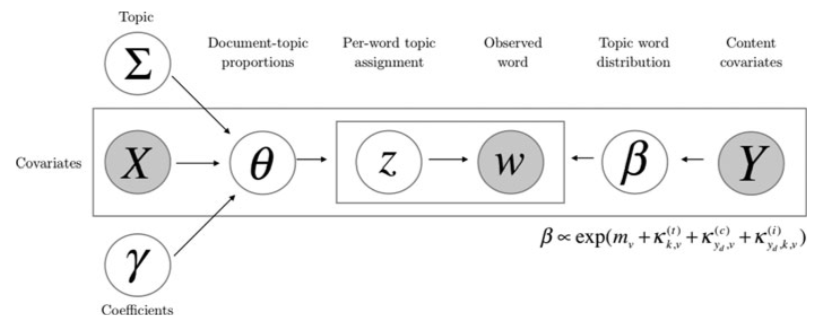
\includegraphics[scale = 0.5]{../plots/2/stm_graphical.png}
  \caption{Graphical model representation of the STM (from \cite{roberts2016model}, p.\ 990).}
  \label{fig:graphical_model}
\end{figure}

\subsubsection*{Scope}

Topic models are unsupervised learning methods, since the true topics from which the text was generated are not known. They have been traditionally used as an exploratory tool providing a concise summary of topics and ideally inducing a good decomposition of the corpus. Topic models have also been applied to tasks such as collaborative filtering and classification (see, e.g.,\ \citealp{blei2003latent}). In particular, they can be employed as dimensionality reduction method in semi-supervised learning methods. Such a process can in general be described as a two-stage approach, where in the first stage topic proportions and content are learned and in the second stage a supervised method such as regression takes this learned representation as input. 

The fundamental idea of the STM is to directly incorporate metadata information in order to discover the topical structure. As with other topic models, the learned structure can then be used to conduct further analysis, such as regression modeling. Since the topic proportions are latent random variables it is preferable to incorporate the uncertainty of $\boldsymbol{\theta}_d$, accessible through the estimated approximation of their posterior, when determining the effect of covariates on topic proportions. This is achieved by what is called the "method of composition" in social sciences. In section \ref{Metadata Analysis - Topical Prevalence and Content} we provide a detailed discussion of this method.

Though not mentioned by the authors of the STM, it is furthermore possible to directly assess the output of an estimated STM that reflects the association of metadata with topics. By doing so, no second step is performed in order to investigate the topic-metadata relationship. In section \ref{Direct assessment} we show how the results of such an analysis differ from the results obtained by a two-stage approach.

The incorporation of metadata in the STM also proves useful if the objective is to examine causality, thus moving beyond mere relationships between metadata and topics. In line with \cite{egami2018make}, we address this issue in section \ref{Causal Inference: Train-test Split}, where we split our data into a training and a test set. We show that the design of the STM allows metadata covariates from the training set to directly help predict topic proportions on the test set.

\subsubsection*{Posterior Distribution}

Before addressing inference and parameter estimation within the STM in section \ref{Inference and Parameter Estimation} below, we briefly derive the posterior distribution of the STM (up to proportionality), as stated on p.\ 992 of \cite{roberts2016model}. Recall that only words $\boldsymbol{W}$,\footnote{We denote the total input of words by $\boldsymbol{W}$, which can, for instance, be represented by the so-called \textit{document-term matrix}, where each of the $D$ rows corresponds to a document, with the $v$-th entry, $v \in \{1, \dots, V\}$, displaying the count of the $v$-th term within this document.} prevalence covariates $\boldsymbol{X}$, and the content covariate $\boldsymbol{Y}$ are observable, while unnormalized topic proportions $\boldsymbol{\eta}$ and topic assignments $\boldsymbol{z}$ are latent and topic-word distribution deviations $\boldsymbol{\kappa}$, prevalence coefficients $\boldsymbol{\Gamma}$, and unnormalized topic proportion variance $\boldsymbol{\Sigma}$ are parameters to be estimated. The posterior is then given by
\begin{align*}
p(\boldsymbol{\eta}, \boldsymbol{z}, \boldsymbol{\kappa}, \boldsymbol{\Gamma}, \boldsymbol{\Sigma} | \boldsymbol{W}, \boldsymbol{X}, \boldsymbol{Y}) & \propto \underbrace{p(\boldsymbol{W} | \boldsymbol{\eta}, \boldsymbol{z}, \boldsymbol{\kappa}, \boldsymbol{\Gamma}, \boldsymbol{\Sigma}, \boldsymbol{X}, \boldsymbol{Y})}_{=p(\boldsymbol{W} | \boldsymbol{z}, \boldsymbol{\kappa}, \boldsymbol{Y})} p(\boldsymbol{\eta}, \boldsymbol{z}, \boldsymbol{\kappa}, \boldsymbol{\Gamma}, \boldsymbol{\Sigma} | \boldsymbol{X}, \boldsymbol{Y}) \\
& \propto p(\boldsymbol{W} | \boldsymbol{z}, \boldsymbol{\kappa}, \boldsymbol{Y}) p(\boldsymbol{z} | \boldsymbol{\eta}) p(\boldsymbol{\eta} | \boldsymbol{\Gamma}, \boldsymbol{\Sigma}, \boldsymbol{X}) \prod p(\boldsymbol{\kappa}) \prod p(\boldsymbol{\Gamma}) \\
& \propto \Big\{ \prod_{d=1}^{D} p(\boldsymbol{\eta}_d | \boldsymbol{\Gamma}, \boldsymbol{\Sigma}, \boldsymbol{x}_d) \Big( \prod_{n=1}^{N} p(w_{d,n} | \boldsymbol{\beta}_{d, n}) p(\boldsymbol{z_{d,n}} | \boldsymbol{\theta}_d) \Big) \Big\} \prod p(\boldsymbol{\kappa}) \prod p(\boldsymbol{\Gamma}) \\
& \propto \Big\{ \prod_{d=1}^{D} \text{Normal}(\boldsymbol{\eta}_d | \boldsymbol{\Gamma}^T\boldsymbol{x}_d^T, \boldsymbol{\Sigma}) \Big( \prod_{n=1}^{N} \text{Multinomial}(\boldsymbol{z}_{n,d}| \boldsymbol{\theta}_d) \\
& \ \ \ \ \times \text{Multinomial}(w_{d,n} | \boldsymbol{\beta}_{d,n}) \Big) \Big\} \times \prod p(\boldsymbol{\kappa}) \prod p(\boldsymbol{\Gamma}),
\end{align*}
where $\boldsymbol{\beta}_{d, n} \in \mathbb{R}^V$ is the topic-word distribution for word $n$ in document $d$ which has been assigned to topic $k$ through $\boldsymbol{z_{d,n}}$. The topic-word distribution vectors $\boldsymbol{\beta}_{k,a}$ have entries $\beta_{k,a,v} \propto \exp(m_{v} + \kappa_{k,v}^{(t)} + \kappa_{a,v}^{(c)} + \kappa_{k, a,v}^{(i)})$, $v \in \{1,\dots,V\}$, where $\kappa_{k,v}^{(t)}$, $\kappa_{a,v}^{(c)}$, and $\kappa_{k, a,v}^{(i)}$ are the log-transformed rate deviations of word $v$ for topic $k$, for content variable level $a$, and for the interaction of $k$ and $a$, respectively.

\subsection{Inference and Parameter Estimation}
\label{Inference and Parameter Estimation}

In this section, we briefly describe how inference and parameter estimation for topic models, in particular for the STM, are performed. Inference is conducted using variational inference, where specifically a variational Expectation-Maximization (EM) algorithm is employed for empirical parameter estimation. As a detailed discussion of the underlying workings is outside the scope of this paper, we refer the reader to the appendix and the referenced papers.

Since the STM, as well as all models it builds on, are (hierarchical) Bayesian models, the central challenge we face is the exact determination of the posterior distribution. Recall that in the section above, we derived the posterior \textit{up to proportionality}, neglecting the division by marginal distributions. The exact posterior distribution is intractable to compute due to the marginal distributions in the denominator, which is why exact inference is infeasible and variational inference is used instead. Generally, for a model with latent variables $\theta$ and $z$ and observable data $x$, variational inference involves approximating the posterior $p(\theta,z|x)$ by postulating a simple distribution family $q(\theta,z)$ for the (joint) distribution of latent model variables $\theta$ and $z$ and subsequently determining the member of this family which minimizes the "distance" to the true posterior distribution, measured using the Kullback-Leibler (KL) divergence (\citealp{wang2013variational}). The approximations of variational inference bring a great amount of flexibility, but come at the cost of some bias, since the approximative distribution family usually does not contain the true posterior.

In the appendix, we show that minimizing KL divergence between true posterior $p$ and the approximating variational distribution $q$ is equivalent to maximizing a lower bound on $\log p(x)$, the log-likelihood of the observed data x. This lower bound is called \textit{ELBO} and is defined as
\begin{align*}
ELBO := \mathbb{E}_q[\log p(\theta,z,x)] - \mathbb{E}_q[\log q(\theta,z)],
\end{align*}
whose second component, $\mathbb{E}_q[\log q(\theta,z)]$, is the entropy of the approximate distribution $q$. To be precise, maximizing \textit{ELBO} (or minimizing KL divergence) refers to finding the governing parameter of the approximating distribution $q$ which maximizes \textit{ELBO}.

The optimality conditions resulting from maximizing \textit{ELBO} lead to the \textit{coordinate ascent algorithm} for variational inference (\citealp{wang2013variational}), which converges towards a local optimum (\citealp{bishop2006pattern}). However, this algorithm only works for \textit{conditionally conjugate} models, such as the LDA: all nodes in this model - in particular, the Dirichlet distribution for drawing topic proportions, the multinomial distribution for assigning topics, and the multinomial for eventually picking words - are conditionally conjugate. The STM, however, as well as the CTM before it, are non-conjugate models due to the logistic normal distribution used to sample topic proportions, which is why algorithm updates are not feasible and the algorithm is not (directly) applicable. As a remedy, \cite{wang2013variational} developed Laplace variational inference, which uses Laplace approximations within coordinate ascent algorithm updates and this way enables the application of the coordinate ascent algorithm for the broader class of nonconjugate models, in particular for CTM and STM.

As stated above, the STM uses an Expectation-Maximization (EM) algorithm for empirical parameter estimation. In the E-step, the variational posterior distributions for topic proportions and assignment, $q(\boldsymbol{\theta}_d)$ and $q(\boldsymbol{z_{d,n}})$, respectively, are updated using Laplace variational inference and coordinate ascent. In the M-step, the model parameters - specifically topical prevalence and content coefficients - are updated by maximizing \textit{ELBO} with respect to them (\citealp{roberts2016model}).
\section{Data}
\label{Data}

\subsection{Data Collection}
\label{Data Collection}

The current political landscape of Germany consists of six parties: the right-wing \textit{AfD}, the Greens (\textit{Bündnis 90/Die Grünen}), the Christian Democrats (\textit{CDU/CSU}), the Left Party (\textit{Die Linke}), the liberal \textit{FDP}, and the Social Democrats (\textit{SPD}). These parties are represented in the German parliament (\textit{Bundestag}) according to the votes obtained during the 2017 German federal election (\textit{Bundestagswahl}), which took place on September 24, 2017. The legislative period amounts to 4 years, thus ending around September 2021. The parliament currently contains a total of 709 seats. For the large majority of the 709 members of the German parliament (\textit{Abgeordnete}), information about their electoral district (\textit{Wahlkreis}) is available.

In order to analyze German political entities based on text data, we constructed a broad database containing personal and Twitter data on an MP level as well as socioeconomic and election data on an electoral-district level, as detailed in the rest of this section. While parts of this database were used in the subsequent topic model analysis, it is also to be used in future text-based analyses regarding German politics. As a first step in constructing the database, we gathered personal information on all German MPs. Using the \textit{BeautifulSoup} web scraping tool (\citealp{richardson2007beautiful}) in the Python programming language (\citealp{van1995python}) as well as a selenium webdriver, we gathered data such as name, party, biographical information, electoral district, and social media accounts from the official parliament website\footnote{https://www.bundestag.de/abgeordnete} for all of the 709 members of the German parliament during its 19th election period, elected on September 24, 2017.\footnote{As of March 30, 2020, the official parliament website contained information on 730 MPs. This is because MPs who resigned or passed away since the beginning of the election period are also listed on the website. These MPs were manually excluded from further analysis.} An additional source of personal MP-level information would be the MPs' personal homepages. However, after inspecting some of these personal homepages at random, we found that there is no systematic way to scrape them. Furthermore, hardly any of these websites contain any informative text data comparable to tweets or Facebook posts. As a consequence, we decided against further pursuing this potential source of information. Due to difficulties and recent restrictions when scraping Facebook data, caused in parts by the aforementioned data scandal, we also discarded Facebook as source of text data and focused solely on Twitter. 

Since information on social media profiles was scarce and incomplete on the official parliament website, we additionally scraped official party homepages of all of the six political parties represented in the current parliament.\footnote{The official homepage of the AfD party does not provide the Twitter profiles of their members, which is why for this party we had to manually gather the account names.} MPs who did not provide a Twitter account either on the official parliament website or on their party's official homepage were excluded. Using Python's \textit{tweepy} library to access the official Twitter API, we scraped all tweets by German MPs from September 24, 2017 through April 24, 2020, i.e., during a total of 31 months. The \textit{tweepy} library offers a variety of additional features to be extracted apart from the mere tweet texts, such as the number of followers of an account, retweets, or how many times a tweet was like or retweeted. While we only use original tweets in the analysis presented in this paper, we included the most relevant additional Twitter features in our database, for use in future analyses. This initially yielded 342,542 tweets from a total of 470 members of parliament.\footnote{\textit{tweepy} restricts the total number of tweets retrievable to 3,200. For those MPs who tweeted more than 3,200 tweets during our period of analysis, the most recent 3,200 tweets were taken into account. However, this only applied to two MPs.}

To complement personal and Twitter data, we also gathered socioeconomic data such as GDP per capita and unemployment rate as well as 2017 election results on an electoral-district level for all of the 299 electoral districts from the official electoral website\footnote{https://www.bundeswahlleiter.de}. After removing the only MP labeled as independent (\textit{fraktionslos}) on the official electoral website as well as 19 MPs without a specific electoral district assigned to them (for matchability with socioeconomic data), the final dataset counted 450 MPs. Overall, 63\% of all 709 MPs were thus included in the analysis. The corresponding total number of tweets amounted to 323,740. For those MPs without elecotoral district, electoral district-level socioeconomic variables could potentially be imputed by using state averages or values of nearby and/or similar districts. However, given that this only applies to 19 out of the remaining 450 MPs and since imputing covariates would introduce further uncertainty, we decided to exclude those MPs.

The table below shows total monthly tweet frequencies for our period of analysis, September 24, 2017 through April 24, 2020. As can be seen, tweet frequencies - though fluctuating - show an increasing trend over time, peaking at almost 20,000 in March 2020. The decrease for April 2020 can partly be explained by the fact that only the first 24 days of the month were taken into account.

\begin{figure}[h!]
  \centering
  \captionsetup{justification=centering,margin=2cm}
  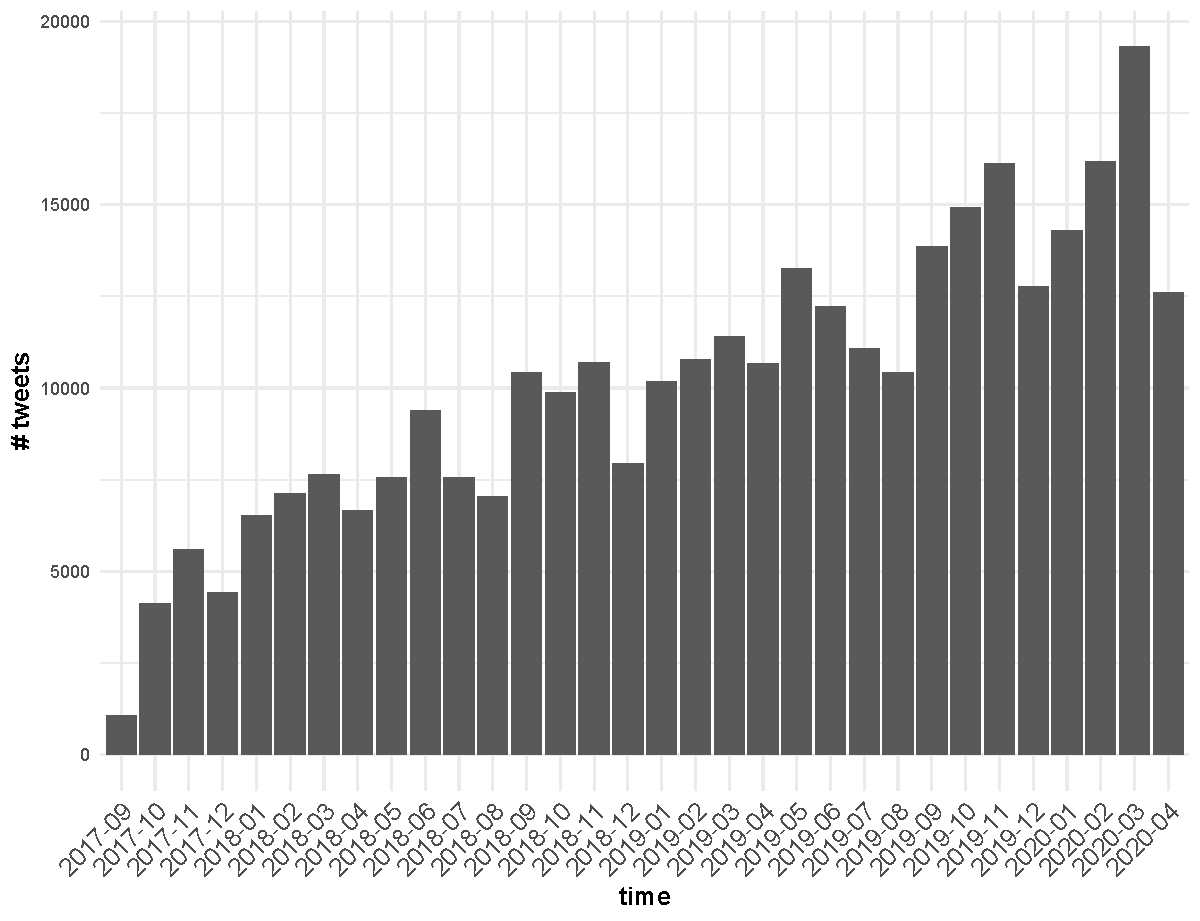
\includegraphics[scale = 0.5]{../plots/3/monthly_tweets.pdf}
  \caption{Monthly tweet volume by German MPs from September 24, 2017 through April 24, 2020.}
  \label{fig:monthly_tweets}
\end{figure}

Next, data was grouped and tweets were concatenated on a per-user level (thus aggregating tweets across the entire 31 months) as well as on a per-user per-month level, yielding a user-level and a monthly dataset. This means that a document represents the concatenation of \textit{all} of a single MP's tweets for the user-level dataset, while it represents a single MP's \textit{monthly} tweets for the monthly dataset. This also means that MP-level metadata such as personal information and socioeconomic data (through the electoral-district matching) can be used as document-level covariates. For the monthly dataset, the temporal component (year and month) constitutes an additional covariate. Since it is reasonable to assume that the importance of topics varies over time and due to resulting documents being shorter and more easily interpretable, we chose the monthly dataset for further analysis.\footnote{For instance, as stated in section \ref{Labeling}, one topic is about COVID-19, which is clearly a relatively recent topic. The monthly dataset allows for tracing the development of this topic's relevance over time: a flat curve until January 2020, followed by a sharp increase during the first months of 2020. The user-level dataset, on the other hand, would simply assign a low overall proportion to this topic.} At this point, the data preparation was completed, marking the starting point of the preprocessing required for topic analysis, which is identical for both the user-level and the monthly dataset.

\subsection{Data Preprocessing}
\label{Data Preprocessing}

For preprocessing, we used the \textit{quanteda} package (\citealp{quanteda}) within the R programming language (\citealp{R}). As a first step, we built a quanteda corpus from all documents. Next, we immediately transcribed German umlauts \textit{ä/Ä}, \textit{ö/Ö}, \textit{ü/Ü} as well as German ligature \textit{ß} as \textit{ae/Ae}, \textit{oe/Oe}, \textit{ue/Ue}, and \textit{ss}, respectively, and removed hyphens. Subsequently, we transformed the text data into a quanteda document-feature matrix (DFM), which essentially tokenizes texts, thereby converting all characters to lowercase. From the DFM, we removed an extensive list of German stopwords, using the stopwords-iso GitHub repository\footnote{https://github.com/stopwords-iso/stopwords-iso}, as well as English stopwords included in the \textit{quanteda} package. Moreover, hashtags, usernames, quantities and units (e.g., \textit{10kg} or \textit{14.15uhr}), interjections (e.g., \textit{aaahhh} or \textit{ufff}), terms containing non-alphanumerical characters, meaningless word stumps (e.g., \textit{innen} from the German female plural declension, or \textit{amp}, the remainder left after removing the ampersand sign, \textit{\&}) were removed. Terms with less than four characters and terms with a term frequency (overall number of occurrences) below five or with a document frequency (number of documents containing the word) below three were excluded. Finally, we manually removed overly frequent terms that would diminish the distinguishability of topics, such as \textit{bundestag} or \textit{polit} (see \textit{semantic coherence} in section \ref{Hyperparameter Search and Model Fitting} for a technical explanation).

We also performed word-stemming, which means cutting off word endings to remove discrepancies arising purely from declensions or conjugations, being of particular importance for the German language. Due to the nature of the German language, the additional gains of lemmatization (which aims at identifying the base form of each word) would only be small as compared to the large increase in complexity, which is why we decided to use stemming only. Another issue when dealing with German language documents is represented by compound words, which are sometimes hyphenated, basically leading to a distinction where semantically there is none. We addressed this issue by removing hyphens in the very beginning of the preprocessing and converting all terms to lowercase, thus "gluing together" compound words; this way, terms like \textit{Bundesregierung} and \textit{Bundes-Regierung} are both transformed into \textit{bundesregierung} (and, after stemming, into \textit{bundesregier}). Finally, automatic segmentation techniques were not necesssary for the German language (\citealp{lucas2015computer}). As a result of preprocessing, one empty MP-level document was dropped, so that a total of 10,998 (monthly) MP-level documents were eventually analyzed, each one associated with 90 covariates.
\documentclass[12pt]{article}
%\usepackage[latin1]{inputenc}
\usepackage[T1]{fontenc}
\usepackage{geometry}
\usepackage{graphicx}
\usepackage{subcaption}
\usepackage[onehalfspacing]{setspace}
\usepackage{amsmath,amsfonts,amssymb,amsthm}
\usepackage{bm}
\usepackage{commath}
\usepackage{enumerate}
\usepackage{accents}
%\usepackage{enumitem}
\usepackage[shortlabels]{enumitem}
\usepackage{dsfont}
\usepackage{mathtools}
\usepackage{physics}
\usepackage{cite}
\usepackage[round]{natbib}
\usepackage{caption}
\captionsetup[figure]{font=small}
\usepackage{float}
\usepackage{hyperref}

\newtheorem*{theorem}{Theorem} 
\newtheorem*{lemma}{Lemma}
\newtheorem*{definition}{Definition}
\newtheorem*{corollary}{Corollary}
\newtheorem*{remark}{Remark}
\newtheorem*{example}{Example}
\newtheorem*{examples}{Examples}
\newcommand*{\QEDB}{\hfill\ensuremath{\square}}

\DeclareMathOperator*{\argmax}{arg\,max}
\DeclareMathOperator*{\argmin}{arg\,min}

\newcommand\independent{\protect\mathpalette{\protect\independenT}{\perp}}
\def\independenT#1#2{\mathrel{\rlap{$#1#2$}\mkern2mu{#1#2}}}

\interfootnotelinepenalty=10000
\allowdisplaybreaks
\geometry{
  left=2.5cm,
  right=2.5cm,
  top=2cm,
  bottom=2cm,
}

\graphicspath{{C:/Users/Simon/OneDrive/Uni/LMU/SS 2020/Statistisches Consulting/Bundestag-MP-Analyse/plots/}}

\begin{document}

\section{Results}

\subsection{Hyperparameter Search and Model Fitting}

Throughout this topic analysis we use the \textit{stm} package, which is implemented in the R programming language (\citealp{stm}). The most important hyperparameter choice when fitting an STM is the number of topics, $K$. While there is no \textit{true} or \textit{optimal} number of topics, we explore the hyperparameter space using the \textit{searchK} function to get an understanding of the impact of $K$ on model fit. We use four of the metrics that come with this function, \textit{held-out likelihood}, \textit{semantic coherence}, \textit{exclusivity}, and \textit{residuals}.

The \textit{held-out likelihood} approach is based on document completion. The \textit{searchK} function randomly holds out a proportion of some of the documents; both the number of documents from which a portion is held out and the respective held-out proportions can be specified by the user. This gives rise to a set of held-out words, for which the likelihood is calculated, given the trained model. Thus, the higher this held-out likelihood, the more predictive power the model has on average. For more detailed information on held-out likelihood based on document completion and other types of held-out likelihoods, see \cite{wallach2009evaluation}.

Regarding the second metric, first introduced by \cite{mimno2011optimizing}, a model with $K$ topics is \textit{semantically coherent} whenever those words that characterize a specific topic $k$ (i.e., the most frequent words within topic $k$) also do appear in the same documents. In order to formally define semantic coherence, let first $D(v)$ be the \textit{document frequency} of word $v$ (that is, the number of documents where $v$ occurs at least once) and let $D(v, v')$ be the \textit{co-document frequency} of words $v$ and $v'$ (that is, the number of documents where both $v$ \textit{and} $v'$ occur at least once). Furthermore, consider the $M$ most probable words in a given topic $k$. Then, semantic coherence for topic $k$, $C_{k}$, is defined as follows:

\begin{align*}
C_{k} &= \sum_{i=2}^{M}\sum_{j=2}^{i-1}\log(\frac{D(v_{i}, v_{j})+1}{D(v_{j})}).
\end{align*}

That is, semantic coherence is the sum of (logarithmized) proportions of word co-occurrences to total word occurrences, the additive factor $1$ in the numerator just being a smoothness adjustment. It becomes apparent that by having some words that are very frequent across a couple of documents, we could achieve high semantic coherence without our topics being semantically coherent at all once we look beyond those common words (\citealp{stm, mimno2011optimizing}). As a partial remedy, we previously excluded some of these overly frequent words (see section 3.2).

A natural "counter-metric" of semantic coherence is \textit{exclusivity}, which basically tells us to which degree a topic's words \textit{only} occur in that topic. To be specific, for a given word $v\in{V}$, the empirical frequencies of $v$ in topic $k$, $\beta_{k,v}$, are normalized across all topics $k\in\{1,...,K\}$. This way, these normalized frequencies now represent the probability of observing topic $k$, conditional upon the word being $v$ - that is, the exclusivity of word $v$ regarding topic $k$. Formally, exclusivity of word $v$ to topic $k$, $E_{k,v}$, is thus defined as:

\begin{align*}
E_{k,v} &= \beta_{k,v}/\sum_{j=1}^{K}\beta_{j,v}.
\end{align*}

Combining a word's frequency and exclusivity finally yields its Frequency-Exclusivity (\textit{FREX}) score, explained in more detail in section 4.2 below (\citealp{bischof2012summarizing}).

Finally, \textit{residuals} is a metric based on residual dispersion. Recall that $z_{d,n}$ is drawn from a $K$-category multinomial distribution, which is a member of the exponential family. Therefore, its dispersion parameter is equal to one, according to theory. This way, an observed residual dispersion larger than one roughly indicates that the number of topics $K$ was most likely chosen insufficiently small. See \cite{taddy2012estimation} for a detailed derivation.

Another aspect to be taken into account when choosing $K$ (or, to be precise, when choosing a search grid for searchK) is interpretability. While a large $K$ certainly allows for a more fine-grained determination of topics, the resulting topics might be rather difficult to label. Furthermore, for large $K$ we would obtain many topics which could be considered sub-topics of the topics we would obtain when using a smaller value for $K$. As a consequence, we select a search grid between 5 and 40, in steps of 5.

Before we can fit the model, we need to choose the document-level covariates we want to include. Since a topic model is explorative by definition, we simply include those covariates that seem to be most influential \textit{a priori}: party and state (both categorical), date (as smooth effect), as well as percentage of immigrants, GDP per capita, unemployment rate, and the 2017 election results of the MP's respective party (the last four as smooth effects and on an electoral-district level). We choose degrees of freedom (df) = 5 for all smooth effects to avoid spurious wiggles due to overfitting. No topical content variable is included at this stage.

The graph below shows the four metrics, as introduced above, for values of $K$ between 5 and 40 (in steps of 5).

\begin{figure}[h!]
  \centering
  \captionsetup{justification=centering,margin=2cm}
  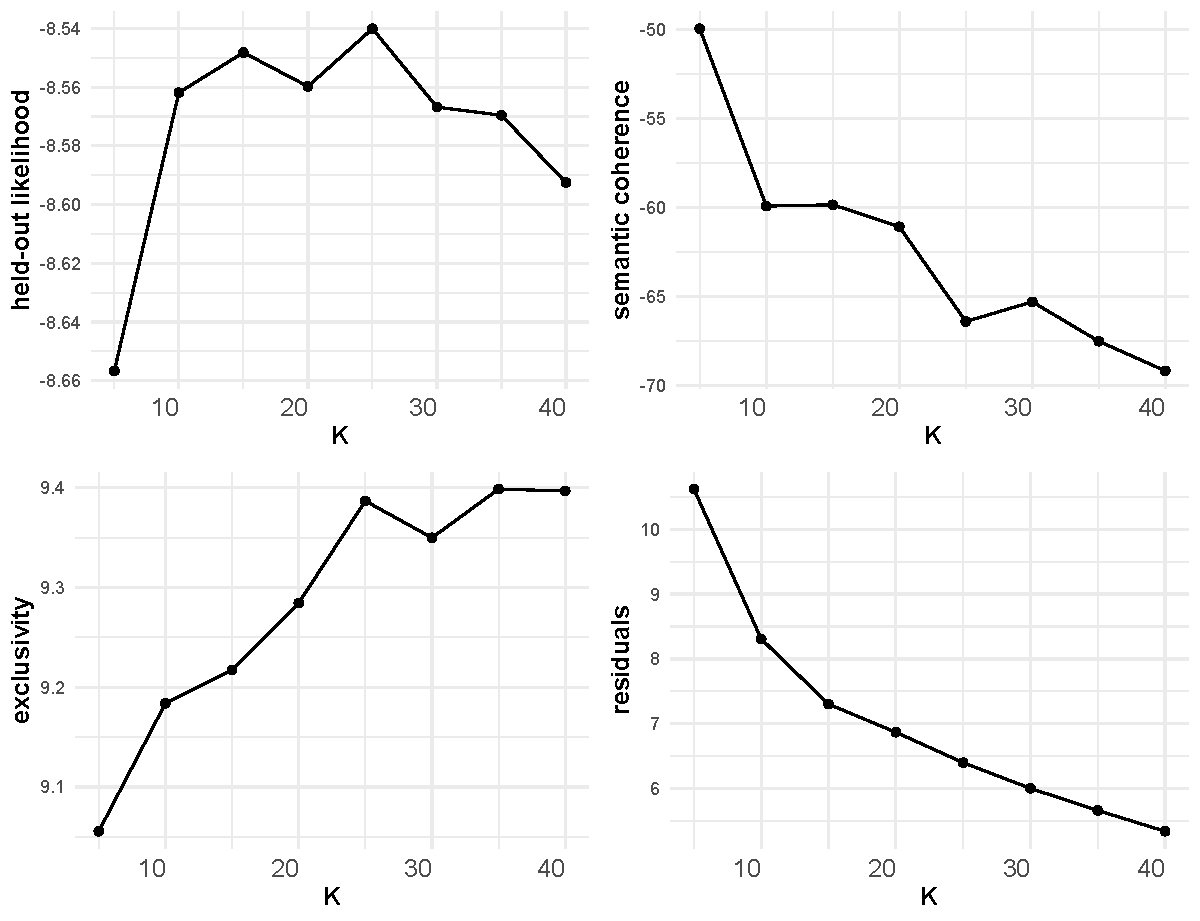
\includegraphics[scale = 0.5]{4_1/searchK.pdf}
  \caption{Model evaluation metrics for hyperparameter K (number of topics).}
  \label{fig:searchK}
\end{figure}

Both 15 and 20 topics seem to be good trade-offs between the metrics used. As mentioned above, no true or optimal $K$ exists. Taking into account the interpretability aspect, we opt for $K$ = 15. For comparison, we also conducted the subsequent analysis for $K$ = 6 and $K$ = 20. In general, the topics generated are similar, but for $K$ = 6 only around three of them are clear-cut, while for $K$ = 20 some topics could easily be grouped together. This further corroborates our choice that $K$ = 15 indeed seems to be a good trade-off. 

Our model thus uses $K$ = 15 as hyperparameter. In order to fit it, we again need to choose document-level covariates. We initially select the same model specifications as in the hyperparameter search above (see sections 4.5 and 4.6 for modifications).

\subsection{Labeling}

As a first step after fitting the model, we would like to visually inspect the resulting topics, in particular their most representative words. However, representativeness of words for a given topic depends on the weighting metric used. The STM comes with four topic-word metrics - \textit{highest probability}, \textit{FREX}, \textit{Lift}, and \textit{Score} - which are discussed in the following.

Given a topic $k$, \textit{highest probability} simply outputs those words in the topic-specific word vector $\beta_{k}$ with the highest corpus frequency, i.e, those with the highest absolute frequency across all documents. Using the same notation as in section 4.1 above, let $\beta_{k,v}$ again be the (empirical) frequency of word $v$ within topic $k$. Then the highest probability word within topic $k$ is simply $\underset{v \in V}{\operatorname{argmax\beta_{k,v}}}$. This relatively simple measure only takes into account how often words occur in absolute terms, but not how specific those words are to the given topic. This is why we observe words like \textit{wichtig}, \textit{berlin}, or \textit{frag} within the highest probability words for several topics. And since such words are very common, unspecific words, they are not particularly useful for distinguishing or labeling topics.

To also account for the degree to which a word \textit{exclusively} belongs to a certain topic, we also consider the top words according to the \textit{FREX} metric. It takes into account not only how frequent but also how exclusive words are. Formally, the FREX score of word $v$ with respect to topic $k$ is calculated as follows:

\begin{align*}
FREX_{k,v} &= (\frac{\omega}{ECDF(\beta_{k,v}/\sum_{j=1}^{K}\beta_{j,v})} + \frac{1-\omega}{ECDF(\beta_{k,v})})^{-1} &= (\frac{\omega}{ECDF(E_{k,v})} + \frac{1-\omega}{ECDF(\beta_{k,v})})^{-1},
\end{align*}

where $\omega$ is the weight  assigned to exclusivity (set to 0.7 by default in the STM), $E_{k,v}$ is the word's exclusivity as defined in section 4.1, and \textit{ECDF} is the empirical CDF. Thus, for a given topic, $FREX_{k,v}$ is simply the harmonic mean of i) the rank of word $v$ by probability within topic $k$ (frequency rank) and ii) the rank of topic $k$ by the frequency of word $v$, across all topics $j \in \{1,...,K\}$ (exclusivity rank). Further information on the estimation of \textit{FREX} can be found in \cite{stm} and in \cite{bischof2012summarizing}.

\textit{Lift} is another topic-word metric, where the frequency of word $v$ within topic $k$,  $\beta_{k,v}$, is weighted by the inverse of $v$'s relative frequency across the entire corpus, i.e., $v$'s empirical corpus probability. Formally:

\begin{align*}
Lift_{k,v} &= \beta_{k,v}/(\omega_{v}/\sum_{v}\omega_{v}).
\end{align*}

where $\omega_{v}$ denotes the word count of word $v$ in the entire corpus. This way, Lift gives higher weight to those words that rarely appear in other topics. Further information on Lift can be found in \cite{taddy2012estimation}.

Finally, the \textit{Score} metric for word $v$ and topic $k$ is formally defined as:

\begin{align*}
Score_{k,v} &= \beta_{k,v}(\log\beta_{k,v} - 1/K\sum_{j}^{K}\log\beta_{j,v})
\end{align*}

Thus, Score weights word $v$'s frequency within topic $k$, $\beta_{k,v}$, by the difference between $v$'s log frequency within topic $k$ and the average of $v$'s log frequencies across all $K$ topics. This can roughly (but not exactly) be seen as: $\beta_{k,v}$ is weighted by the proportion of $v$'s log frequency within topic $k$ to $v$'s average logarithmic frequency across all topics. For further information on the Score metric, see the R package \textit{lda} (\cite{chang2010package}).

To get a broad overview of which words characterize each one of the topics, the output below shows the five top words according to each of the four topic-word evaluation metrics, for three selected topics (see appendix XXX for top words of all topics).

\vspace{0.5cm}
\noindent
\textit{Topic 1 Top Words:}\\
 	 \textbf{Highest Prob:} buerg, link, merkel, frau, sich \\
 	 \textbf{FREX:} altpartei, islam, linksextremist, asylbewerb, linksextrem \\
 	 \textbf{Lift:} eitan, 22jaehrig, abdelsamad, abgehalftert, afdforder \\
 	 \textbf{Score:} altpartei, linksextremist, frauenkongress, islamist, boehring \\
\textit{Topic 3 Top Words:}\\
 	 \textbf{Highest Prob:} brauch, wichtig, leid, dank, klar \\
 	 \textbf{FREX:} emissionshandel, soli, marktwirtschaft, feedback, co2steu \\
 	 \textbf{Lift:} aequivalenz, altersvorsorgeprodukt, bildungsqualitaet, co2limit, co2meng \\
 	 \textbf{Score:} emissionshandel, co2limit, basisrent, euet, technologieoff \\
\textit{Topic 6 Top Words:}\\
 	 \textbf{Highest Prob:} gruen, klimaschutz, brauch, klar, euro \\
 	 \textbf{FREX:} fossil, erneuerbar, kohleausstieg, verkehrsminist, verkehrsw \\
 	 \textbf{Lift:} abgasbetrug, abgebaggert, abschalteinricht, abschaltet, ammoniak \\ 
 	 \textbf{Score:} erneuerbar, fossil, zdebel, verkehrsminist, klimaschutz \\
\vspace{0.5cm}

A key task of topic analysis is to actually ascribe a meaning to the topics identified, i.e., labeling them. While this is clearly where human judgment should and does come into play, we attempt to conduct the labeling in a more strategic (and thus less subjective) manner, following a 3-step procedure. This procedure is exemplified using topic 1. First, we consider the \textit{words} contained in the topic, for instance by simply inspecting the top words (see output above). For a better visualization, we use a word cloud. As shown below, for a given topic (i.e., conditional upon a specific topic being chosen), it shows highest probability words weighted by their frequency. For instance, by judging at first sight topic 1 appears to be about right-wing nationalist issues, particularly immigration.

\begin{figure}[h!]
  \centering
  \captionsetup{justification=centering,margin=2cm}
  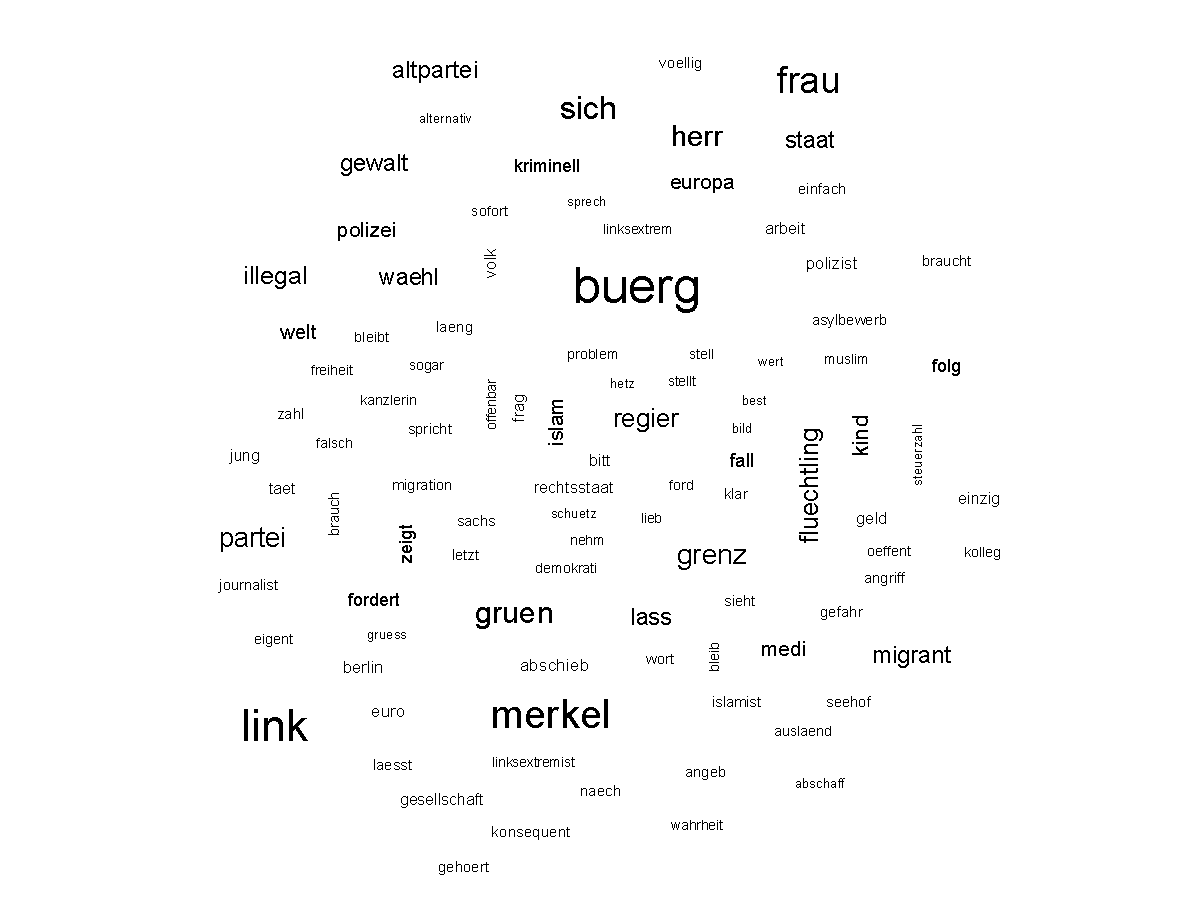
\includegraphics[scale = 0.5]{4_2/t1_wordcloud.pdf}
  \caption{Word cloud for topic 1.}
  \label{fig:t1_wordcloud}
\end{figure}

Second, to get a more thorough insight into the topic, we take a look at those documents that show the highest proportion for topic 1; that is, we consider the corresponding original, unedited tweets. The most representative document for topic 1 has a topic proportion $\theta_1$ equal to 98.86\%. It contains tweets from MP Martin Hess, a member of the AfD party from Baden-Württemberg, during June 2018. That is, MP Martin Hess tweeted almost exclusively about topic 1 during June 2016. The monthly document starts with:

\vspace{0.5cm}
\noindent
\textit{"Ehem. Verfassungsrichter bestätigt AfD-Forderung: Zurückweisung illegaler Migranten dringend geboten. Gegenwärtige Politik widerspricht dem Verstand und auch der Verfassung. Wir müssen zurück zu Recht \& Ordnung, wie die \#AfD seit fast 3 Jahren fordert!"}
\vspace{0.5cm}

The second most representative document for topic 1, with an almost identical $\theta_1$ = 98.37\%, is from the same MP, this time from May 2018. The document begins with:

\vspace{0.5cm}
\noindent
\textit{"Mio-Überweisungen u.a. an Kanzleien unter \#BAMF-Außenstellenleiterin, die mit Anwälten bandenmäßig Asylbetrug begangen haben soll. Und die Frau ist noch frei und präsentiert sich als Gutmensch. \#Staatsanwaltschaft muss hier handeln und Haftgründe prüfen."}
\vspace{0.5cm}

The documents exclusively focus on immigration issues, confirming the first impression gained through top words and word cloud: topic 1 concerns right-wing nationalist issues, in particular immigration. As a third step in our labeling process we finally label the topic: in this case, as "Right/Nationalist". We repeat this 3-step procedure (inspecting top words and word cloud, reading through top documents, assigning a 1- or 2-word label) for all remaining topics, arriving at the following manual labels:

\begin{table}[h!]
	\centering
	\captionsetup{justification=centering,margin=2cm}
	\begin{tabular}{|l|l|}
	\hline
	Topic1  & Right/Nationalist    \\ \hline
	Topic2  & Miscellaneous 1      \\ \hline
	Topic3  & Climate Economics    \\ \hline
	Topic4  & Social/Housing       \\ \hline
	Topic5  & Digital/Future       \\ \hline
	Topic6  & Climate Protection   \\ \hline
	Topic7  & Europe               \\ \hline
	Topic8  & Corona               \\ \hline
	Topic9  & Left/Anti-war        \\ \hline
	Topic10 & Twitter/Politics 1   \\ \hline
	Topic11 & Twitter/Politics 2   \\ \hline
	Topic12 & Miscellaneous 2      \\ \hline
	Topic13 & Twitter/Politics 3   \\ \hline
	Topic14 & Right-wing Extremism \\ \hline
	Topic15 & Society/Solidarity   \\ \hline
	\end{tabular}
	\caption{List of topic labels.}
	\label{Tab:labels}
\end{table}

\subsection{Global-level Topic Analysis}

Next, we identify two ways to calculate global topic proportions (for a given topic $k$): either as the simple (unweighted) average of $\theta_{d,k}$ across all documents (i.e., as the average of MP-level proportions across all MPs): $\frac{1}{D}\sum_{d=1}^{D}\theta_{d,k}$; or by first weighting each $\theta_{d,k}$ by the number of words in the respective documents, $N_d$, and then averaging across documents. The table below shows all topics with their respective global proportions for both weighting methodologies. We observe that for most topics, weighted and unweighted proportions are rather similar, but there are exceptions. In particular, the topics concerned with everyday political tweets have much higher unweighted than weighted frequencies; this makes sense, however, since such "diplomatic" tweets tend to be shorter than those discussing a specific content.

\begin{figure}[h!]
  \centering
  \captionsetup{justification=centering,margin=2cm}
  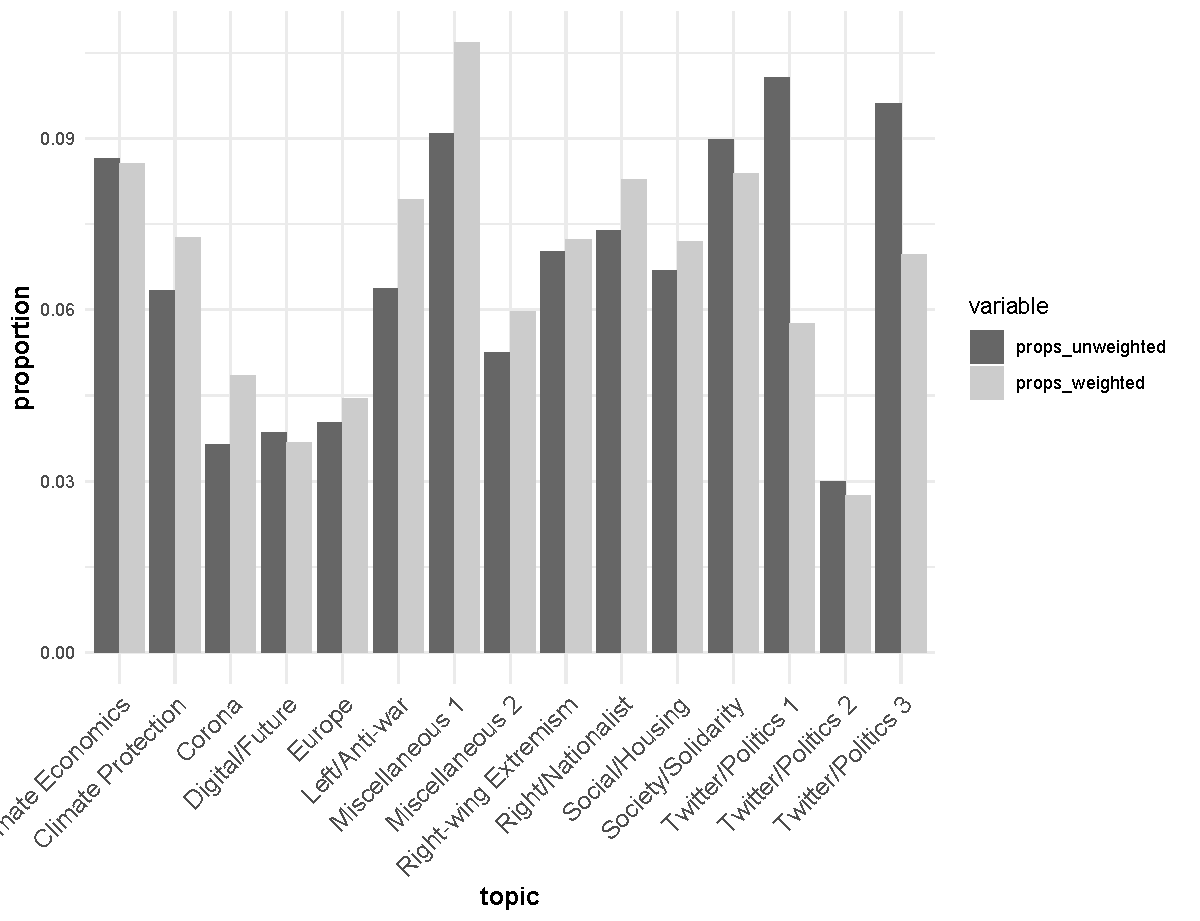
\includegraphics[scale = 0.5]{4_3/global_thetas.pdf}
  \caption{Weighted and unweighted global topic proportions.}
  \label{fig:global_thetas}
\end{figure}

While labeling tells us which words best represent each topic - and thus, what each topic truly represents - it does not yet tell us to which extent individual topics are related to each other. In the graph below, we visualize the similarity of two topics, Topic 3 (Climate Economics) and Topic 6 (Climate Protection), in terms of their vocabulary usage. As suggested by the topic labels already, there is a significant overlap in vocabulary usage.

\begin{figure}[h!]
  \centering
  \captionsetup{justification=centering,margin=2cm}
  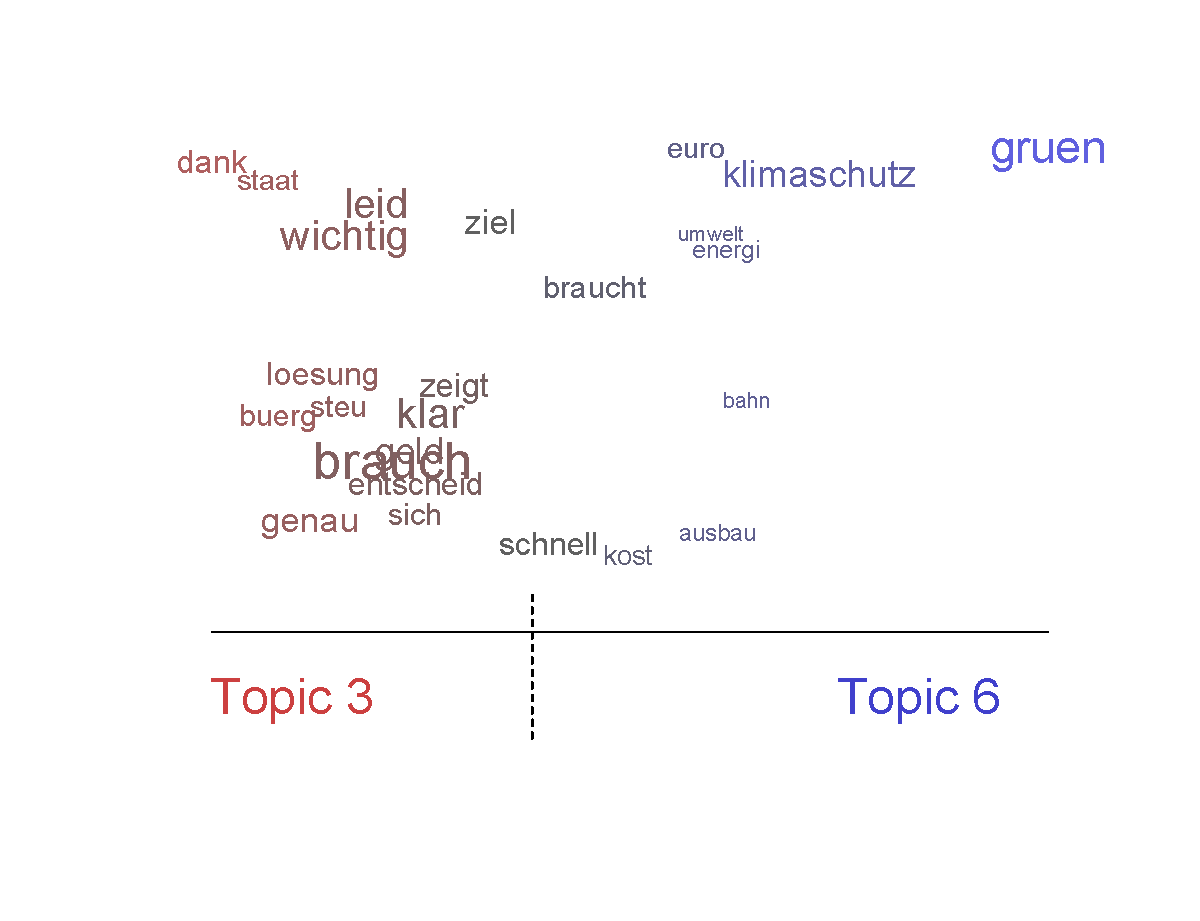
\includegraphics[scale = 0.5]{4_3/vocabulary_comparison.pdf}
  \caption{Comparison of vocabulary usage for two topics.}
  \label{fig:vocabulary_comparison}
\end{figure}

More generally, we can evaluate the connectedness between different topics by means of a matrix of correlations between document-level topic proportions $\theta_d$. This is visualized in the graph below (left panel). Most topics are negatively correlated with each other, which does not come as a surprise, given the relatively low total number of topics, 15, and that topic proportions are “supplements”: the higher one topic proportion, the lower the total of the others. Moreover, most topic correlations are rather weak in absolute size: the strongest negative correlation (-19.84\%) is the one between topic 1 (Right/Nationalist) and topic 15 (Society/Solidarity), while the strongest positive correlation (11.79\%) is the one shown before, between topic 3 (Twitter/Politics 1) and topic 6 (Twitter/Politics 3). We can also visualize these correlations using a network graph (right panel), where topics are connected by a dashed line whenever they are positively correlated. We observe three small clusters as well as some isolated topics, one of them being topic 8, Corona, which makes sense since it only entered the public sphere in early 2020, i.e., during the last months of our data collection period. In general, the relationships between the topics, as depicted below, are in line with their labeling.

\begin{figure}[h!]
  \centering
  \captionsetup{justification=centering,margin=2cm}
  \begin{subfigure}[b]{0.4\linewidth}
    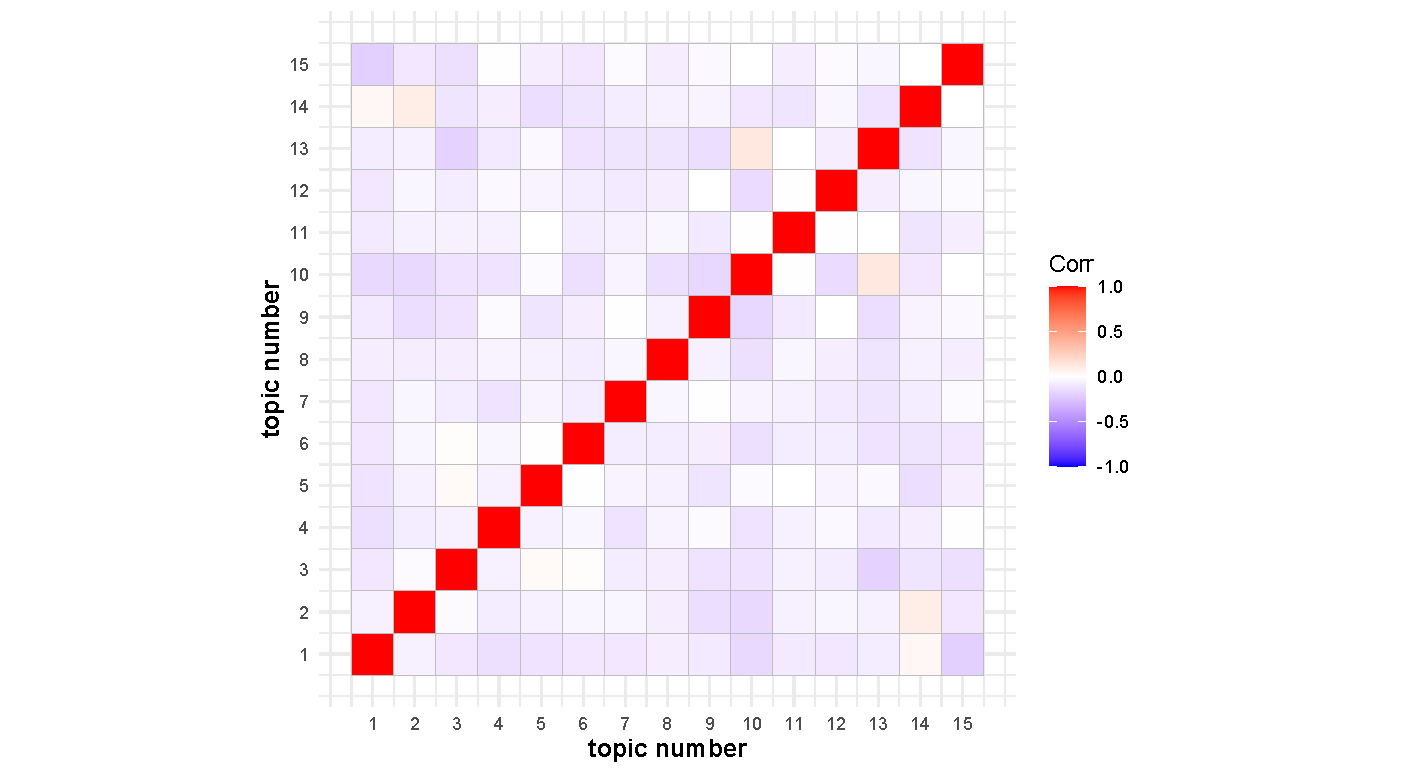
\includegraphics[width=\linewidth]{4_3/topic_correlations.pdf}
  \end{subfigure}
  \begin{subfigure}[b]{0.4\linewidth}
    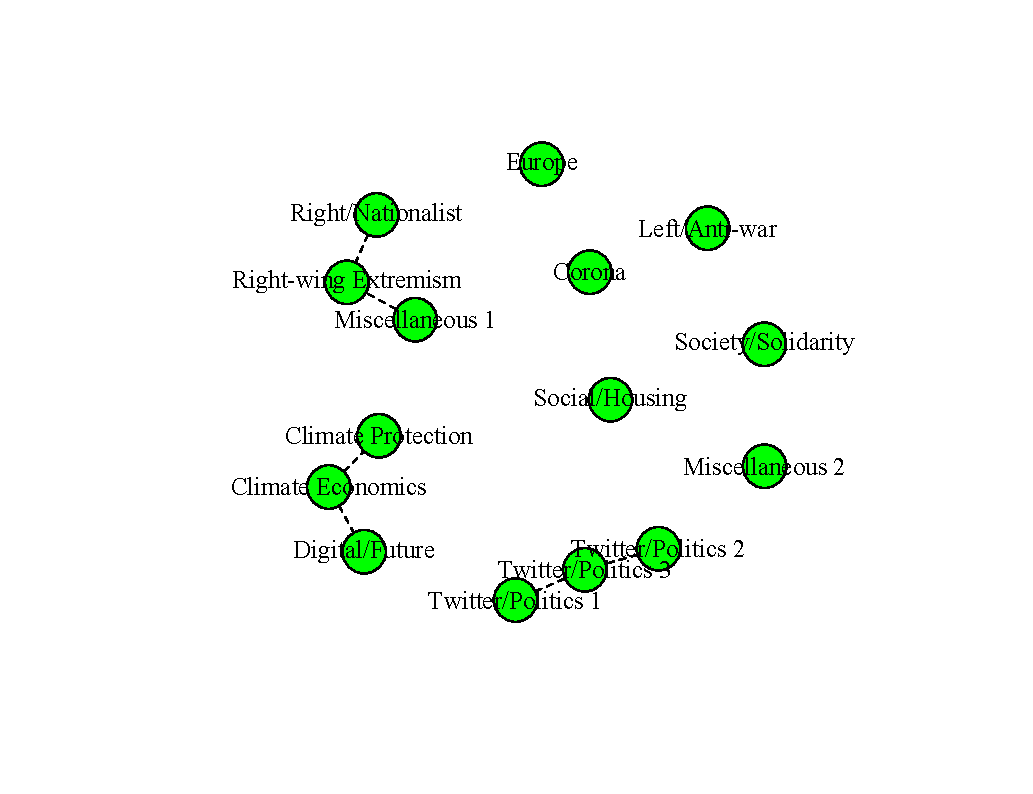
\includegraphics[width=\linewidth]{4_3/topic_correlations_map.pdf}
  \end{subfigure}
  \caption{Global topic correlations as matrix (left) and graph (left).}
  \label{fig:topic_correlations}
\end{figure}

\bibliography{bibliography}
\bibliographystyle{plainnat}

\end{document}
\section{Covariate-level Topic Analysis}

We now proceed to analyze the relationship between metadata information (i.e., document-level covariates) and topic proportions. We specify topical prevalence as 
\begin{align}
\mu_{d,k} = x_d^T \gamma_k= \text{party}_{d,k} + \text{state}_{d,k} + f_k(\text{t}_d) + g_k(\text{struct}_d), \label{prevalence}
\end{align} 
for all documents $d = 1,\dots,D$, and all topics $k = 1,\dots,K$, where 
\begin{align*}
g_k(\text{struct}_d) = g_{k}^{(1)}(\text{GDP}_d)+g_{k}^{(2)}(\text{unemployment}_d)+g_{k}^{(3)}(\text{immigrants}_d)+g_{k}^{(4)}(\text{votes}_d). 
\end{align*} 
That is, the political party and federal state of the respective parliamentarian associated with a document are specified as simple categorial dummy effects, while date and electoral-district structural covariates (GDP per capita, unemployment rate, percentage of immigrants, and the 2017 vote share) are modeled as additive smooth functions.

Note that approximate inference implies replacing $\mu_{d,k}$ with $\lambda_{d,k}$, i.e., with the mean of the approximate Gaussian posterior $q(\eta_{d,k})$. The estimates of $\Gamma = [\gamma_1 | \dots | \gamma_K]$ are updated in a Bayesian linear regression during each iteration of the EM algorithm in the M-step; for details see \cite{roberts2013structural}, p.\ 993.

While topical prevalence has an effect on the estimated topic proportions, the exact specification of topical prevalence is not a decisive factor. Both estimated topic proportions as well as heldout likelihood are in general only marginally affected by the concrete choice of the functional form. However, completely removing topical prevalence, in which case the model reduces to a CTM, does result in different topic proportions, as we show in section XXX. Since evaluation metrics such as heldout likelihood are mostly unaffected by the exact choice of topical prevalence and because the computational cost of fitting an stm is rather high, automatic model selection methods w.r.t.\ topical prevalence are not available. A reasonable specification of topical prevalence therefore relies on the domain knowledge of the researcher.

There exist different approaches to study the relationship between topic proportions and prevalence covariates. One possibility is to directly assess the maximum-a-posteriori (MAP) estimates $\hat{\Gamma}$ and $\hat{\Sigma}$, which are generated by the stm. Since the document-level topic proportions $\theta_d$ follow a logistic normal distribution (with mean $\mu_d$ and covariance matrix $\Sigma$), interpretation of the results can be difficult, since the logistic normal distribution is not very accessible. Nonetheless, we can visualize the relationship between a topic and a prevalence covariate, fixing other covariates at their median (or, for categorial variables, at the majority vote).

Alternatively, the estimated topic proportions can be used as the dependent variable of a new regression on prevalence covariates. However, in contrast to a standard regression setting, in this case the dependent variable has been estimated itself, before the regression is performed. Instead of simply using the MAP estimates of $\theta_d$ as the dependent variable, having access to the posterior distribution of the topic proportions, we can take account for the uncertainty of the dependent variable. This can be achieved by employing a sampling procedure known as the method of composition in the social sciences; see \cite{tanner2012tools}, p.52. This procedure is implemented in the \textit{stm} package through its function \textit{estimateEffect}.

In the following, we will first introduce the method of composition. We will discuss its implementation in the \textit{stm} package and provide alternative regression approaches based on the method of composition. Subsequently, we will evaluate the relationship between prevalence covariates and topic proportions by directly assessing the MAP estimates $\hat{\Gamma}$ and $\hat{\Sigma}$, as outlined above, and compare the results of both approaches.

\subsection{Method of Composition}

Let $\theta_{(k)}:=(\theta_{1,k}, \dots, \theta_{D,k}) \in [0,1]^{D}$ denote the proportions of the $k$-th topic for all $D$ documents. As stated, we want to perform a regression of these topic proportions $\theta_{(k)}$ on a subset $\tilde{X} \in \mathbb{R}^{D \times \tilde{P}}$ of prevalence covariates $X$. The true topic proportions are unknown, but the stm produces an estimate of the approximate posterior of $\theta_{(k)}$. A na{\"\i}ve approach would be to regress the estimated mode of the approximate posterior distribution on $\tilde{X}$. However, this approach neglects much of the information contained in the distribution. 

Instead, repeatedly sampling $\theta_{(k)}^*$ from the approximate posterior distribution, performing a regression for each sampled $\theta_{(k)}^*$ on $\tilde{X}$, and then sampling from the estimated distribution of 
icients, provides an i.i.d.\ sample from the marginal posterior distribution of regression coefficients. 

Sampling $\theta_{(k)}^*$ is achieved by first sampling the unnormalized topic proportions $\eta^*$ from the approximate posterior $q(\eta)$, applying the softmax $\theta^* = \text{softmax}(\eta^*)$ (element-wise, i.e., for each of the K-dimensional vectors of topic proportions), and lastly selecting the $k$-th column of $\theta^*$. Precisely, $q(\eta) = \prod_d q(\eta_d)$ is a normal distribution, which emerges from the laplace approximation within the variational inference scheme; for details see \cite{roberts2016model}, pp.\ 992-993. For clarity, we denote the approximate posterior of topic proportions as $q(\theta_{(k)} | X, W)$, in order to emphasize that the parameters of this distribution are learned from the observed data, i.e.\ prevalence covariates and words (note that we have no content variables included). Furthermore, let $\xi$ denote the regression coefficients from a regression of $\theta_{(k)}$ on $\tilde{X}$, and let $q(\xi| \tilde{X}, \theta_{(k)})$ be the approximate posterior distribution of these coefficients, i.e.\ given design matrix $\tilde{X}$ and response $\theta_{(k)}$.

The method of composition can now be described by repeating the following process $m$ times:
\begin{enumerate}
\item Draw $\theta_{(k)}^* \sim q(\theta_{(k)} | X, W)$.
\item Draw $\xi^* \sim q(\xi | \tilde{X}, \theta_{(k)})$.
\end{enumerate}
It then holds that $\xi_1^*, \dots, \xi_m^*$ is an i.i.d.\ sample from the marginal posterior
\begin{align*}
q(\xi | X, W) := \int_{\theta_{(k)}} q(\xi| \tilde{X}, \theta_{(k)}) q(\theta_{(k)} | X, W) \text{d} \theta_{(k)} = \int_{\theta_{(k)}} q(\xi, \theta_{(k)} | X, W) \text{d} \theta_{(k)}, 
\end{align*}
where $q(\xi, \theta_{(k)} | X, W) := q(\xi| \tilde{X}, \theta_{(k)}) q(\theta_{(k)} | X, W)$. Thus, by integrating over $\theta_{(k)}$, this approach allows incorporating information contained in the posterior distribution of $\theta_{(k)}$ when determining $\xi$.

\subsubsection{Implementation in the \textit{stm} package}

The R package \textit{stm} implements a simple OLS regression through its \textit{estimateEffect} function. However, this approach ignores that the sampled topic proportions are restricted to $(0,1)$. As expected, using this framework we frequently observe predicted proportions outside of $(0,1)$. Moreover, credible intervals are non-informative, due to violated model assumptions. 

\begin{figure}[h!]
  \centering
  \captionsetup{justification=centering,margin=2cm}
  \begin{subfigure}[b]{0.4\linewidth}
    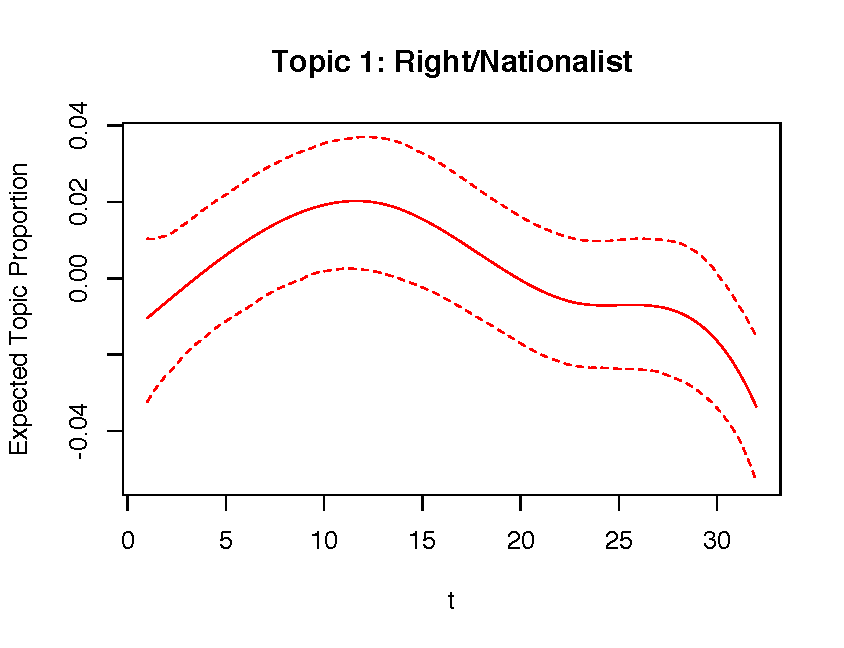
\includegraphics[width=\linewidth]{../plots/4_4/estEffect_topic1.pdf}
  \end{subfigure}
  \begin{subfigure}[b]{0.4\linewidth}
    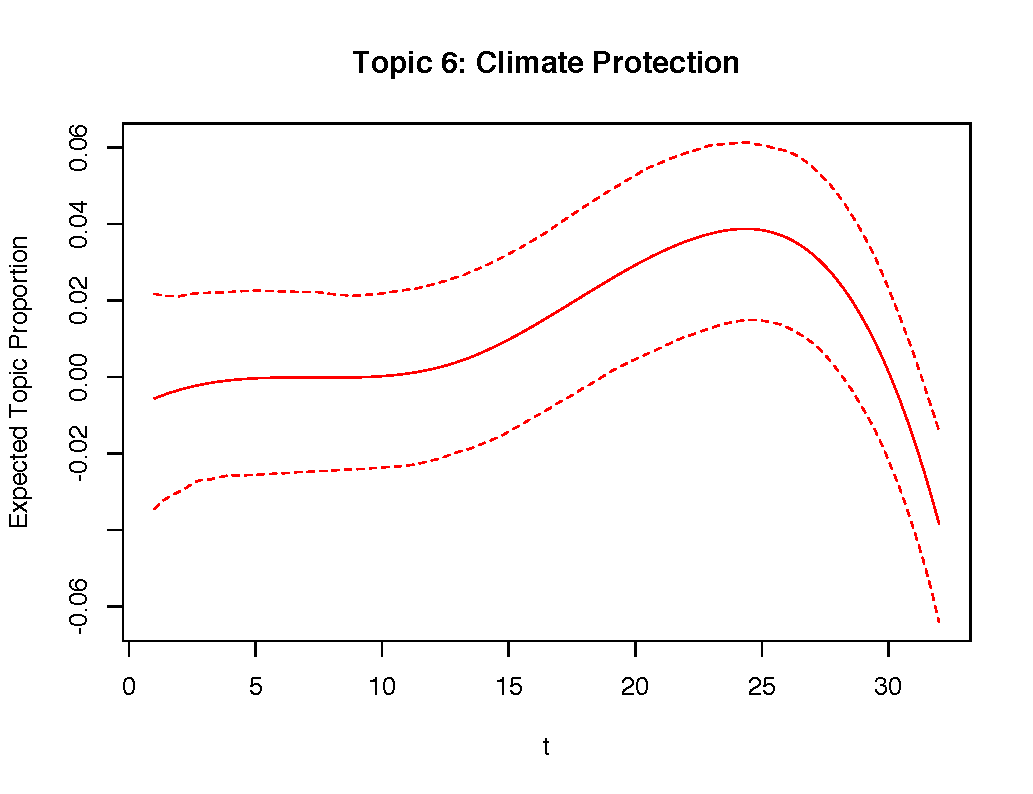
\includegraphics[width=\linewidth]{../plots/4_4/estEffect_topic6.pdf}
  \end{subfigure}
  \caption{Estimated prevalence of topics 1 and 6 over time, generated using \textit{estimateEffect} from the \textit{stm} package}
  \label{fig:coffee}
\end{figure}

\subsubsection{Alternative implementation}

We can attempt to improve the approach employed within the \textit{stm} package by replacing the OLS regression with a regression model that assumes a dependent variable in the interval $(0,1)$. However, note that since topic proportions are modeled separately, regardless of the specific model implied, distributional assumptions about $\theta_{(k)}$ will be violated. This is due to the fact that the the distribution of a subvector - and thus particularly of a single component - of $\theta_d$ is not of a simple form, when $\theta_d$ follows a logistic normal distribution, see e.g.\ \cite{atchison1980logistic}.

As shown by \cite{atchison1980logistic}, a distribution that can be used to approximate a logistic normal distribution is the Dirichlet distribution. However, note that the Dirichlet distribution assumes less interdependence among components than implied by the logistic normal distribution. In case of the Dirichlet distribution the univariate marginal distributions are beta. One possibility is thus to perform a separate beta regression for each topic proportion on $\tilde{X}$. 

As an alternative approximation we can employ a quasibinomial generalized linear model (GLM). Topic proportions can be rescaled and discretized and topics comprehended as classes, such that each rescaled topic proportion can be interpreted as the "number of successes" for the respective class. To match the underlying logistic normal distribution more closely, the quasi-likelihood furthermore allows for a flexible variance specification.

Note that $q(\xi| \theta_{(k)}, \tilde{X})$ is asymptotically normal for both the beta regression, see \cite{ferrari2004beta}, p.\ 17, and the quasibinomial GLM, see e.g.\ \cite{fahrmeir2007regression}, p. 285. Furthermore, in both cases we use a logit-link.

\subsubsection{Visualization}

We now apply the method of composition, based on either a beta regression or a quasibinomial GLM, in order to visualize covariate effects. Here we only visualize the results obtained by the quasibinomial GLM; the results of the beta regression, which show similar trends, are found in the appendix. Setting the number of simulations to 100, we sample $\xi^*_1, \dots, \xi^*_{100}$ from the  marginal posterior distribution $q(\xi | X, W)$. As mentioned, when visualizing the impact of a particular covariate, all other covariates are held at their median (or majority vote, if categorial), in line with the methodology employed in the \textit{stm} package.
Let $\tilde{X}^*$ denote the subset of $X$ where, apart from the variable of interest, each selected column consists of the median of the respective column of $X$. In order to plot the predicted effects, we then input $\tilde{X^*}\xi^*$ into the sigmoid function, which is the response function corresponding to a regression with logit-link, and calculate the predicted proportions. 

We exemplarily illustrate the relationship between covariates and topic proportions for topic 4 ("Social/Housing") and topic 6 ("Climate Protection"). The linear predictor of our regressions takes the same form as in  \eqref{prevalence}, i.e., we do not use a subset $\tilde{X}$, but the full set of prevalence covariates $X$, in order to estimate the effects, although we do not display each covariate included. For smooth effects, it is important to recall that their borders are inherently unstable, which is why one should refrain from (over-)interpreting them. For both continuous and categorical variables, black lines indicate the mean, and the shaded area represents 95\% credible intervals.

\begin{figure}[h!]
  \centering
  \captionsetup{justification=centering,margin=2cm}
  \begin{subfigure}[b]{0.49\linewidth}
    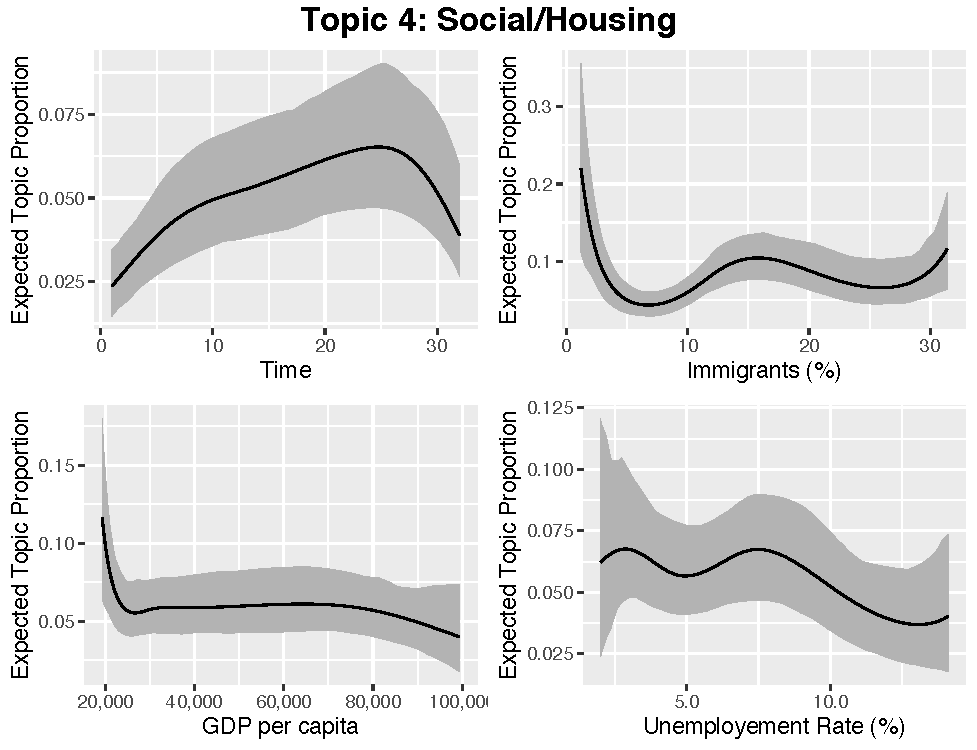
\includegraphics[width=\linewidth]{../plots/4_4/quasi_t4_cont.pdf}
  \end{subfigure}
  \begin{subfigure}[b]{0.49\linewidth}
    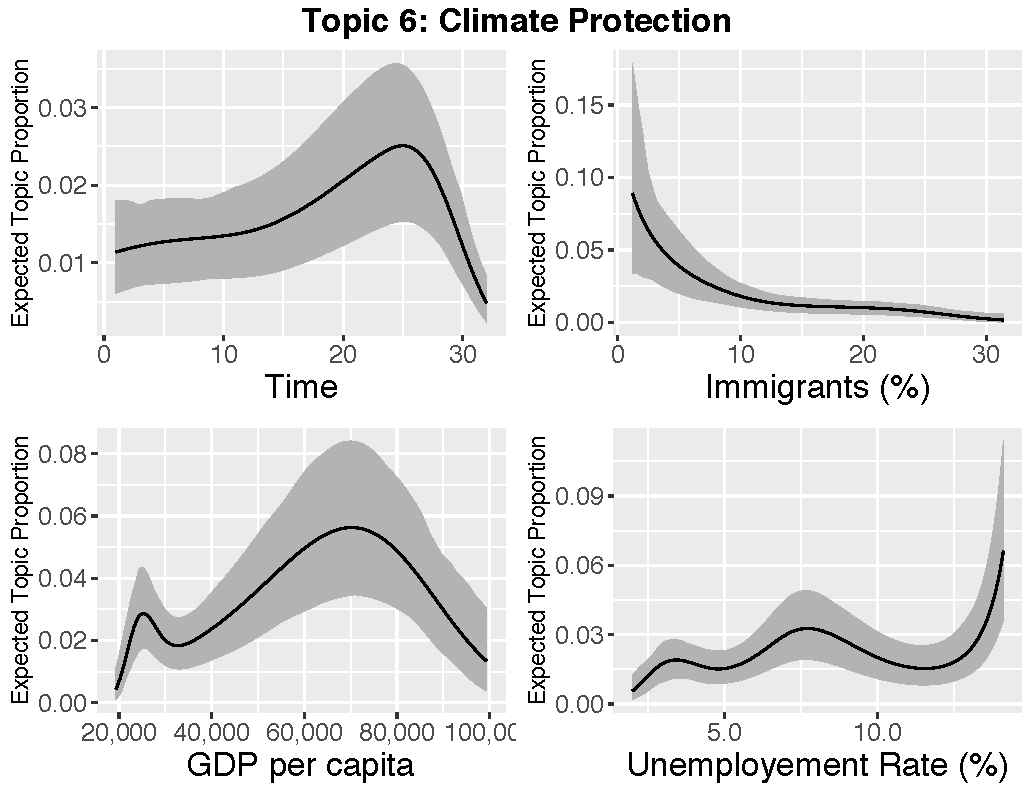
\includegraphics[width=\linewidth]{../plots/4_4/quasi_t6_cont.pdf}
  \end{subfigure}
  \caption{Mean and 95\% credible intervals for smooth effects, obtained using a quasibinomial GLM.}
  \label{fig:coffee}
\end{figure}

\begin{figure}[h!]
  \centering
  \captionsetup{justification=centering,margin=2cm}
  \begin{subfigure}[b]{0.49\linewidth}
    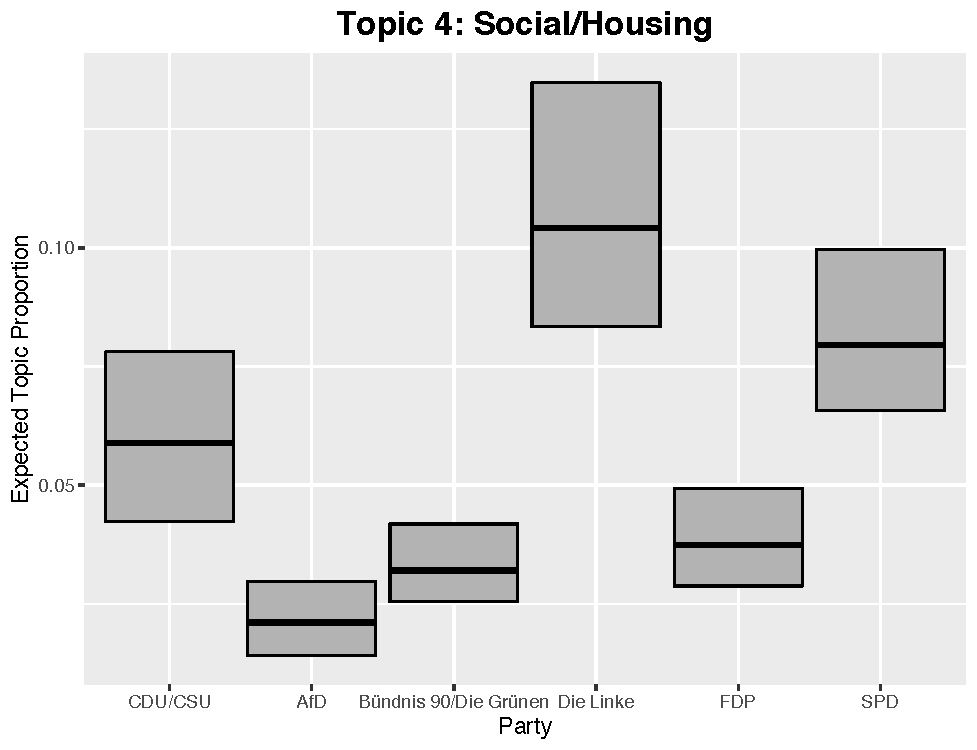
\includegraphics[width=\linewidth]{../plots/4_4/quasi_t4_cat.pdf}
  \end{subfigure}
  \begin{subfigure}[b]{0.49\linewidth}
    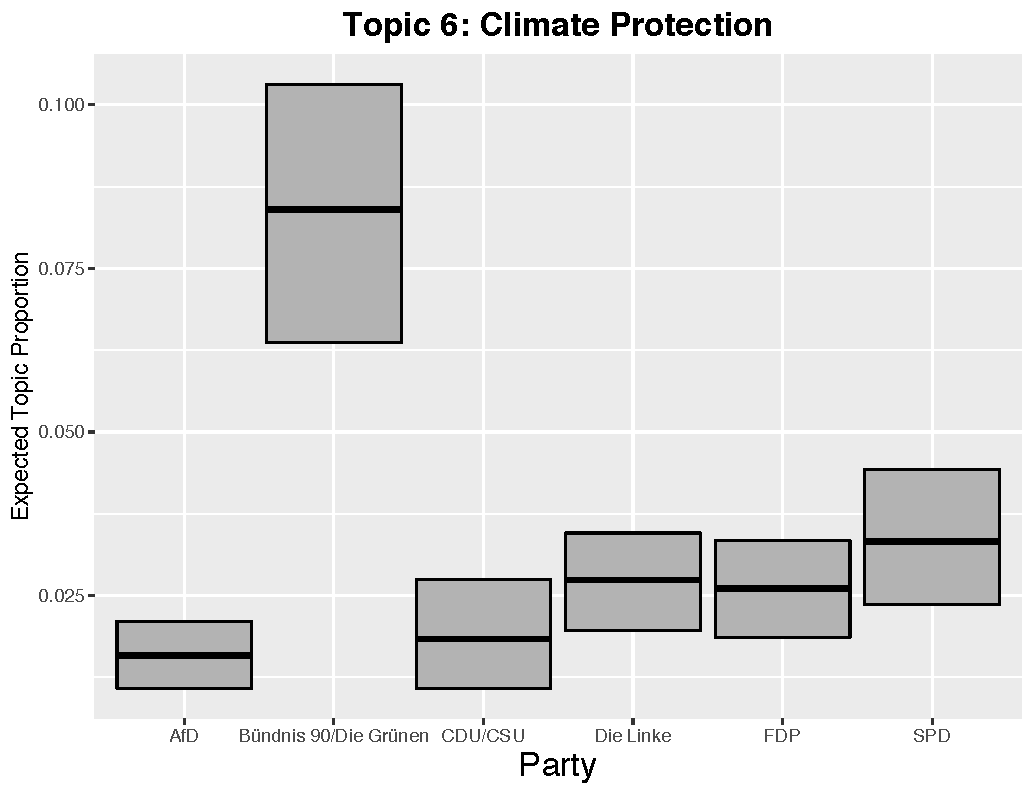
\includegraphics[width=\linewidth]{../plots/4_4/quasi_t6_cat.pdf}
  \end{subfigure}
  \caption{Mean and 95\% credible intervals for different political parties, obtained using a quasibinomial GLM.}
  \label{fig:coffee}
\end{figure}

For topic 4, "Social/Housing", we observe that most continuous variables have a small effect in absolute terms: the absolute variation in topic proportion across the covariate domains merely amounts to 4\%, compared to 8\% for topic 6. For most covariates the trend is rather ambiguous. Somewhat surprisingly, a very high unemployment rate is negatively linked to topic 4.

The effect of the political party on the relevance assigned to the topic "Social/Housing" is very much in line with a priori expectations: the left party and social democrats have the highest topical prevalence (15\% and 10\%, respectively), and the nationalist party the lowest (2\%).

For the smooth effects of topic 6, we observe its prevalence peaks in September 2019, corresponding to month t=25, decreasing afterwards. The absolute changes in topic proportions over time are rather small (around 3\%). The percentage of immigrants within an electoral district shows a negative relation to topic 6. Furthermore, topic 6 tends to be discussed more frequently in mid-income electoral districts than in high- and low-income districts. Finally, the link to the unemployment rate is somewhat ambiguous, although generally rather positive.

Regarding the relationship between the political party and the prevalence of topic "Climate Protection", as to be expected, we find high topical prevalence for the green party. Similar to the smooth effects, total variation in topic proportions across parties amounts to approximately 8\%.

Finally, the graph below shows a summary comparison of topical prevalence across all parties, for topics "Right/Nationalist", "Climate Protection" and "Social/Housing". The results are generally consistent with expectations. The proportions of topics "Climate Protection" and "Social/Housing" vary between 2\% and 9\% and between 2\% and 15\%, respectively. For topic 1, "Right/Nationalist", note how topical prevalence for the AfD party amounts to more than 40\%, implying that more than 40\% of the total content tweeted by AfD party members is about right-wing/nationalist issues, particularly immigration; for all other parties, topic 1 is rather marginal below 3\%.

\begin{figure}[h!]
  \centering
  \captionsetup{justification=centering,margin=2cm}
  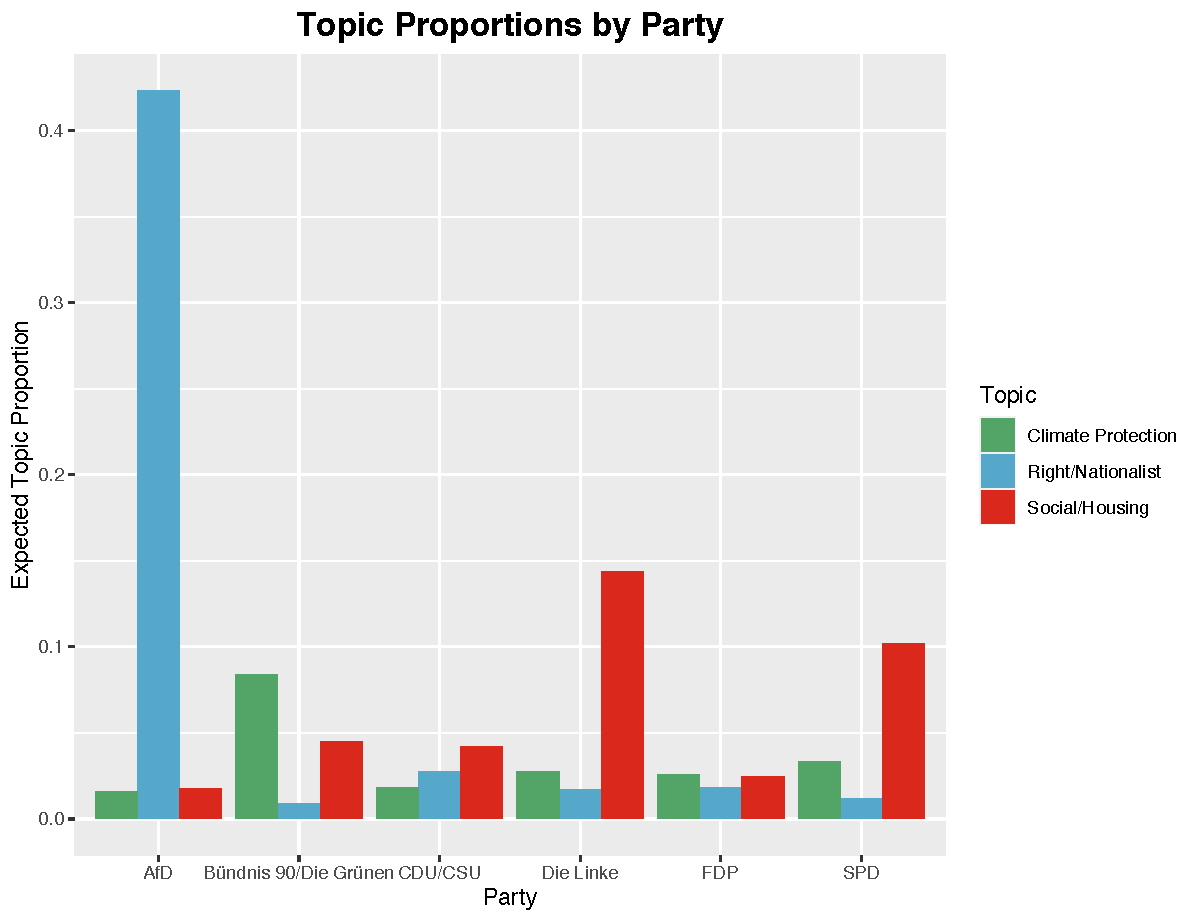
\includegraphics[scale = 0.5]{../plots/4_4/quasi_t146_cat.pdf}
  \caption{Topical prevalence by political party for topics 1, 4, and 6.}
  \label{fig:boat1}
\end{figure}

\subsection{Direct assessment using $\hat{\Gamma}$ and $\hat{\Sigma}$}

The \textit{stm} being an extension to the correlated topic model (\textit{CTM}), it is assumed that the topic proportions follow a logistic normal distribution, such that $\theta_d \sim \text{LogisticNormal}_{K-1}(\Gamma^Tx_d^T, \Sigma)$. Within the CTM, the Dirichlet distribution of the LDA has been replaced with a logistic normal distribution, in order to allow for a joint dependence among topics. Therefore, as mentioned above, separately modeling topic proportions is a simplification; in particular credible intervals should be treated with caution.

In order to examine the relation of prevalence covariates and topic proportions considering the joint dependence among the latter, we can attempt to directly use the output produced by the \textit{stm}: inference of the \textit{stm} involves finding the maximum-a-posteriori (MAP) estimate $\hat{\Gamma}$ and the maximum likelihood estimate $\hat{\Sigma}$. 

If we are interested in the question how a specific prevalence variable is related to topic proportions, similar to previous analyses, we can attempt to predict topic proportions based on a new design matrix $X^*$, where each column apart from the variable of interest corresponds to the median of the respective column of $X$. Ideally, in order to directly predict topic proportions, we would first draw a sample $\Gamma^*$ from the posterior distribution of $\Gamma$, and subsequently sample the topic proportions $\theta_d^*$ from a logistic normal with mean parameters $((\Gamma^*)^T (x_d^*)^T, \hat{\Sigma})$, where $\hat{\Sigma}$ is the maximum likelihood estimation of $\Sigma$. The resulting topic proportions would then correspond to a sample of the posterior predictive distribution of topic proportions. Unfortunately, the output of the stm does not allow for the possibility to draw a sample from the posterior distribution of $\Gamma$, but only provides its MAP estimate $\hat{\Gamma}$. 

Nevertheless, in order to get an impression how the assumed generative process of topic proportions in the stm behaves, we can plug in the estimates $\hat{\Gamma}$ and $\hat{\Sigma}$ into the logistic normal distribution and visualize sampled values from this distribution. Given a new observation $x_d^*$, we can sample $\theta_d^*$ from $\text{LogisticNormal}_{K-1}(\hat{\Gamma}^T(x_d^*)^T, \hat{\Sigma})$ by

\begin{enumerate}
\item Drawing $\eta_d^* \sim \mathcal{N}_{K-1}(\hat{\Gamma}^T(x_d^*)^T, \hat{\Sigma})$ and setting $\eta^*_{d,K} = 0$.
\item Mapping to the simplex, i.e., for all $k = 1,\dots,K$: $\theta_{d,k}^* = \frac{\exp(\eta^*_{d,k})}{\exp(\sum_{i=1}^{K} \eta^*_{d,i})}$.
\item Setting $\theta_d^* := (\theta_{d,1}^*, \dots \theta_{d,K}^*)^T$.
\end{enumerate}

We have repeated the above steps 1000 times for each input value of a selected variable, while fixing other variables at their median, and obtained the empirical mean as well as 95\% credible intervals. Plotting the results, we observe that while the mean shows a similar trend to our precious analyses, the obtained credible intervals are much broader.

\begin{figure}[h!]
    \centering
     \captionsetup{justification=centering,margin=2cm}
  \begin{subfigure}[b]{0.3\linewidth}
    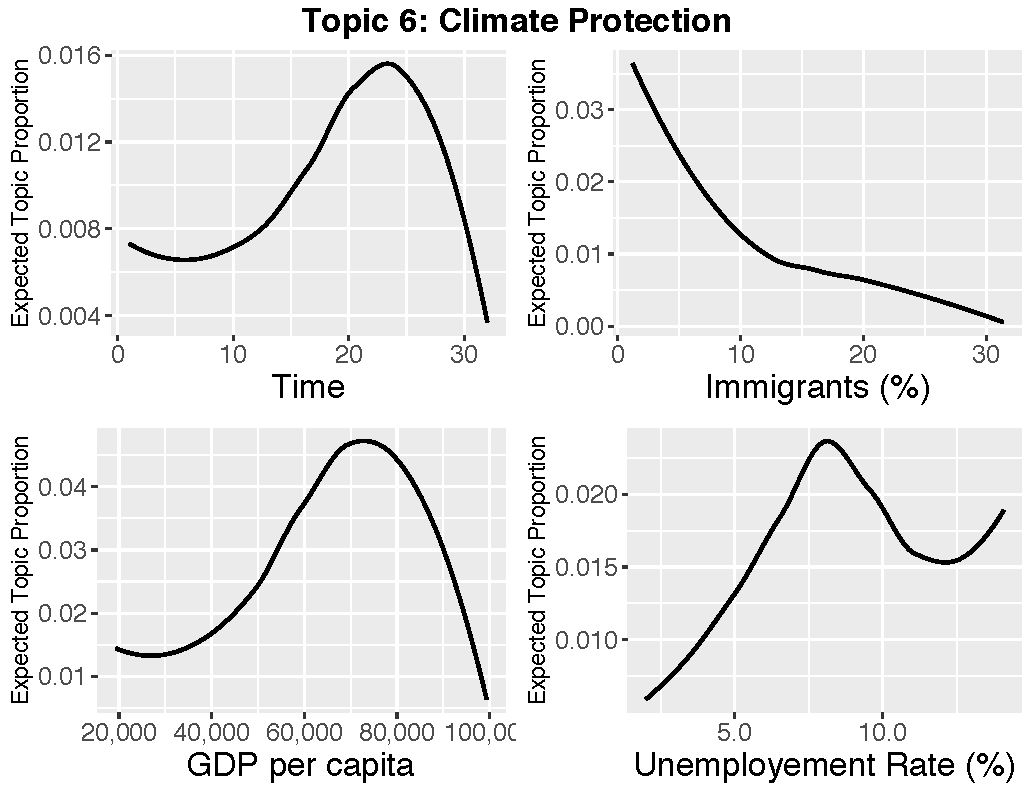
\includegraphics[width=\linewidth]{../plots/4_4/direct_t6_without_credible.pdf}
  \end{subfigure}
  \begin{subfigure}[b]{0.3\linewidth}
    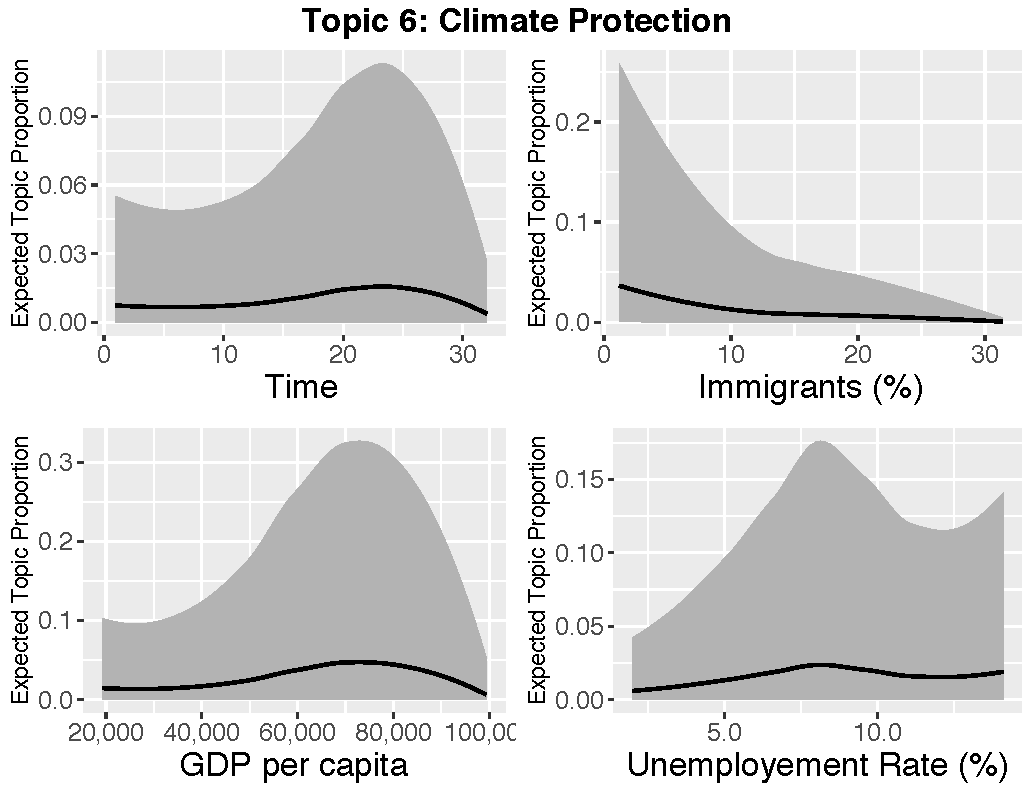
\includegraphics[width=\linewidth]{../plots/4_4/direct_t6_with_credible.pdf}
  \end{subfigure}
  \begin{subfigure}[b]{0.3\linewidth}
    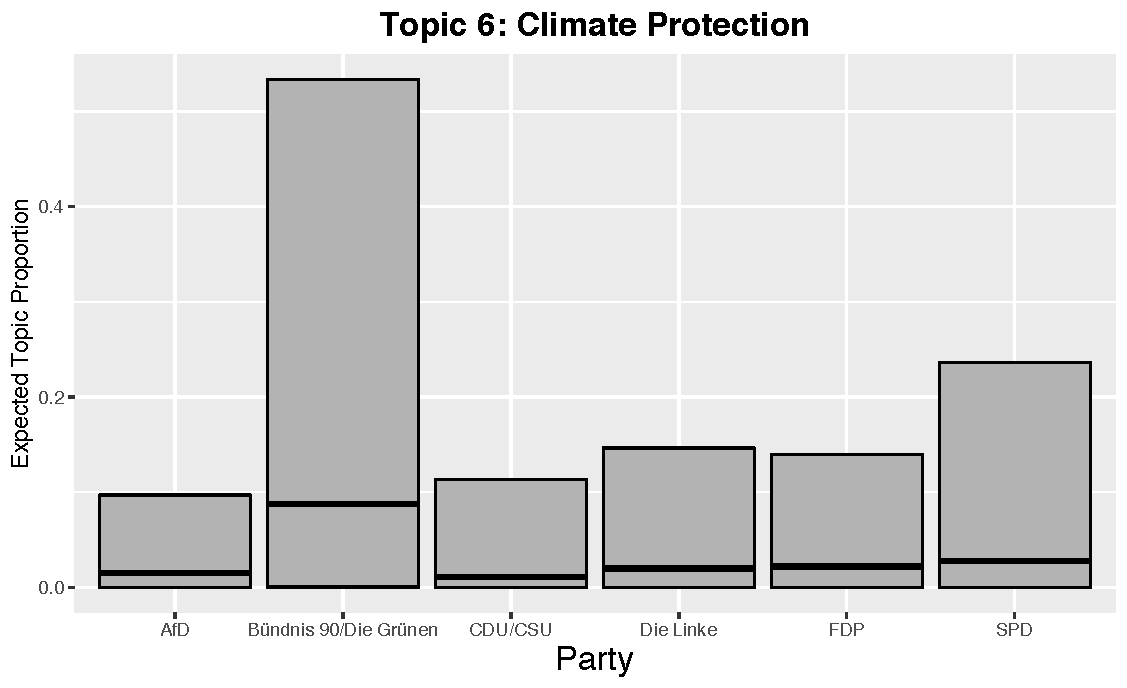
\includegraphics[width=\linewidth]{../plots/4_4/direct_t6_cat.pdf}
  \end{subfigure}
  \caption{Smooth effects without credible intervals, smooth effects with credible intervals and effect of the political party.}
  \label{fig:directassessment}
\end{figure}

The large fluctuations for a specific topic proportion can be ascribed to the fact that the unnormalized topic proportions are drawn from a $K-1$-dimensional \textit{multivariate} normal distribution, before the softmax is applied. Therefore, a single normalized proportion depends heavily on the sampled unnormalized proportions of the remaining topics. While the variance of a topic-specific unnormalized proportion is independent of the remaining unnormalized proportions and c.p.\ constant for an increasing number of topics, the application of the softmax function induces a large increase in the variance of a topic-specific normalized proportion.

We suspect that the magnitude of credible intervals in figure \ref{fig:directassessment} provides a more realistic picture than in case of a separate modeling of topic proportions, since the usage of the logistic normal distribution of topic proportions is an implicit assumption made within the stm that there is a dependence among topics, as argued above. This ultimately produces a large variance of the univariate marginal distributions of topic proportions, as can be observed. While ideally we should sample $\Gamma$ from its posterior distribution instead of plugging in its MAP estimate, our results suggest that there is a discrepancy between the assumed distribution of topic proportions in the generative process of the stm, and the impression we gain of the distribution of topic proportions from a separate modeling of topics within the method of composition.


\documentclass[12pt]{article}
%\usepackage[latin1]{inputenc}
\usepackage[T1]{fontenc}
\usepackage{geometry}
\usepackage{graphicx}
\usepackage{subcaption}
\usepackage[onehalfspacing]{setspace}
\usepackage{amsmath,amsfonts,amssymb,amsthm}
\usepackage{bm}
\usepackage{commath}
\usepackage{enumerate}
\usepackage{accents}
%\usepackage{enumitem}
\usepackage[shortlabels]{enumitem}
\usepackage{dsfont}
\usepackage{mathtools}
\usepackage{physics}
\usepackage{cite}
\usepackage[round]{natbib}
\usepackage{caption}
\captionsetup[figure]{font=small}
\usepackage{float}
\usepackage{hyperref}

\newtheorem*{theorem}{Theorem} 
\newtheorem*{lemma}{Lemma}
\newtheorem*{definition}{Definition}
\newtheorem*{corollary}{Corollary}
\newtheorem*{remark}{Remark}
\newtheorem*{example}{Example}
\newtheorem*{examples}{Examples}
\newcommand*{\QEDB}{\hfill\ensuremath{\square}}

\DeclareMathOperator*{\argmax}{arg\,max}
\DeclareMathOperator*{\argmin}{arg\,min}

\newcommand\independent{\protect\mathpalette{\protect\independenT}{\perp}}
\def\independenT#1#2{\mathrel{\rlap{$#1#2$}\mkern2mu{#1#2}}}

\interfootnotelinepenalty=10000
\allowdisplaybreaks
\geometry{
  left=2.5cm,
  right=2.5cm,
  top=2cm,
  bottom=2cm,
}

\graphicspath{{C:/Users/Simon/OneDrive/Uni/LMU/SS 2020/Statistisches Consulting/Bundestag-MP-Analyse/plots/}}

\begin{document}

\section{Results}

\subsection{Topical Content}

The STM provides an additional way to integrate covariate effects into the model, apart from prevalence variables that impact topic proportions across documents. To be specific, a categorical variable can be selected as topical content variable. While the prevalence variables influence the propensity of the 15 topics for each document, the content variable now allows for the word distributions for a given topic to vary across documents, according to content variable levels. Note that this is a completely new model, which is why one should not expect the resulting topics to be similar. 

Formally, recall that the word distribution used to eventually pick a word is $\beta_{d,n} := \beta(z_{d,n}, Y_d) \in \mathbb{R}^V$, where $z_{d,n}$ is a (latent) indicator variable determining the word's topic assignation and $Y_{d}$ is the document-level topical content variable with $A$ levels. In the prevalence model, no (document-level) topical content variable is specified, implying $\beta_{d,n} = \beta(z_{d,n})$; since $z_{d,n}$ is a word-level variable, $\beta_{d,n}$ is constant across all documents for a given topic $k$. When specifying a content variable $Y$, however, $\beta_{d,n}$ now varies for each document, according to the level $a \in \{1, ..., A\}$ the content variable takes on for document $d$. That is, the total number of $\beta$-vectors, each one of length $V$, now increases from $K$ to $K \times A$.

For our specific case, since the topical content variable needs to be categorical, we choose the variable \textit{party}, being categorical by definition and as it  is arguably the most significant factor in determining topic prevalence. IN doing so, we additionally posit that for a given topic, an MP's party also influences the vocabulary used when tweeting about that specific topic. For instance, this implies that an AfD party member tweets about immigration issues in a different linguistic manner than, say, a green MP. Since for the 2017 election period the German parliament contains members of 6 parties, $\bf{Y}$ is now a matrix with 10998 rows and 6 columns, yielding a total of 90 $\beta$-vectors.

After fitting the model, we proceed as for the prevelance model, that is, by inspecting top words and identifying topic labels. An additional difficulty, however, is that we do not have clear-cut top words per topic anymore; instead, we now have topic-level top words for each of the 15 topics, party-level top words for each of the 6 parties, as well as interaction top words for each of the 90 topic-party combinations. The table below presents topic labels for all 15 topics, identified by using the same 3-step procedure as for the prevalence model before. As can be seen, five topics are labeled as \textit{miscellaneous}, reflecting the complexity caused by the large number of $\beta$-vectors.

\begin{table}[h!]
	\centering
	\captionsetup{justification=centering,margin=2cm}
	\begin{tabular}{|l|l|}
	\hline
	Topic1  & Right/Nationalist 1  \\ \hline
	Topic2  & Miscellaneous 1      \\ \hline
	Topic3  & Left/Humanitarian    \\ \hline
	Topic4  & Housing       	   \\ \hline
	Topic5  & Innovation           \\ \hline
	Topic6  & Green/Energy         \\ \hline
	Topic7  & Miscellaneous 2      \\ \hline
	Topic8  & Corona               \\ \hline
	Topic9  & Foreign Affairs      \\ \hline
	Topic10 & Election             \\ \hline
	Topic11 & Right/Nationalist 2  \\ \hline
	Topic12 & Miscellaneous 3      \\ \hline
	Topic13 & Miscellaneous 4      \\ \hline
	Topic14 & Twitter/Politics     \\ \hline
	Topic15 & Miscellaneous 5      \\ \hline
	\end{tabular}
	\caption{List of topic labels for STM with topical content variable (party).}
	\label{Tab:labels_content}
\end{table}

The topical content model allows for vocabulary usage to differ across political parties, given a topic. In the graph below, we visualize this effect for the Corona topic, contrasting the green party "Bündnis 90/Die Grünen" with the right-wing nationalist party "AfD". The result is very insightful: even for a topic as clear-cut and novel as COVID-19, stark differences in terms of vocabulary usage arise. In particular, the AfD uses language suitable to describe immigration (\textit{migration}, \textit{grenz}) in order to discuss Corona, which very much reflects the unimodality of the party's political orientation. The green party, on the other hand, seems to address the topic much more specifically, mentioning key words like \textit{massnahm} or \textit{kind}.

\begin{figure}[h!]
  \centering
  \captionsetup{justification=centering,margin=2cm}
  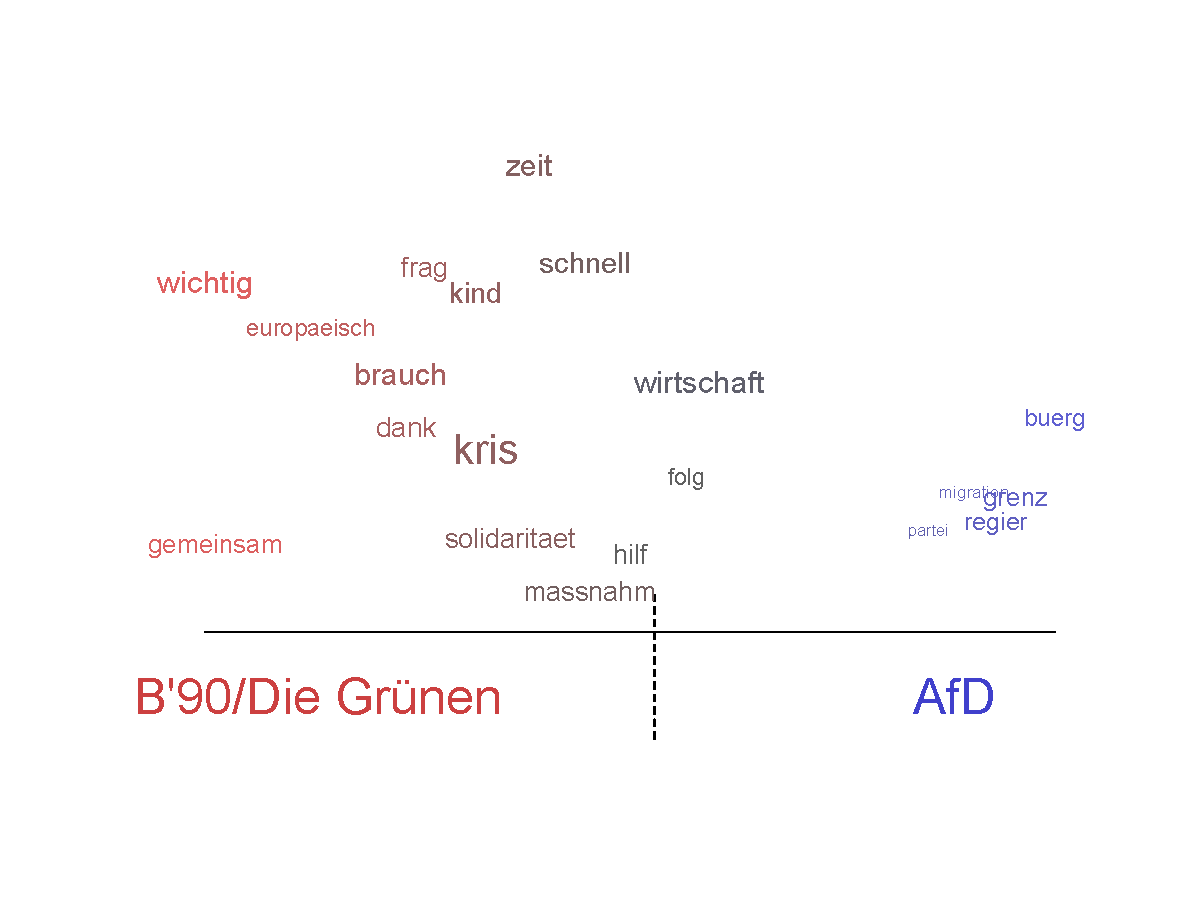
\includegraphics[scale = 0.5]{4_5/t8_vocab_parties.pdf}
  \caption{Differences in vocabulary usage across parties for the Corona topic.}
  \label{fig:t8_vocab_parties}
\end{figure}

While this type of visualization is indeed insightful, several concerns regarding the topical content model prevail: first of all, there is no natural candidate for the content variable, which - for labelling and interpretational purposes - should ideally be binary. Our dataset contains very few categorical variables, none of them binary. Furthermore, there is no natural, non-arbitrary way to binarize any of the covariates; for instance, binarizing the variable party, say, into conservative and liberal would misclassify at least one party. Therefore, our choice to use party as content variable is the result of a lack of alternatives, rather than being based on sound statistical or theoretical considerations. This, in turn, is reflected in the difficult labelling; for instance, one
third of all topics were eventually being labelled as miscellaneous. And while the previous illustration of inter-party differences in vocabulary usage is indeed insightful in terms of topic exploration and visualization, the aforementioned doubts lead us to discard the topical content variable for further analysis. In fact, in the next section we consider a model without any covariates in order to perform a clean 2-step procedure for covariate effect estimation.


\bibliography{bibliography}
\bibliographystyle{plainnat}

\end{document}
\documentclass[12pt]{article}
%\usepackage[latin1]{inputenc}
\usepackage[T1]{fontenc}
\usepackage{geometry}
\usepackage{graphicx}
\usepackage{subcaption}
\usepackage[onehalfspacing]{setspace}
\usepackage{amsmath,amsfonts,amssymb,amsthm}
\usepackage{bm}
\usepackage{commath}
\usepackage{enumerate}
\usepackage{accents}
%\usepackage{enumitem}
\usepackage[shortlabels]{enumitem}
\usepackage{dsfont}
\usepackage{mathtools}
\usepackage{physics}
\usepackage{cite}
\usepackage[round]{natbib}
\usepackage{caption}
\captionsetup[figure]{font=small}
\usepackage{float}
\usepackage{hyperref}

\newtheorem*{theorem}{Theorem} 
\newtheorem*{lemma}{Lemma}
\newtheorem*{definition}{Definition}
\newtheorem*{corollary}{Corollary}
\newtheorem*{remark}{Remark}
\newtheorem*{example}{Example}
\newtheorem*{examples}{Examples}
\newcommand*{\QEDB}{\hfill\ensuremath{\square}}

\DeclareMathOperator*{\argmax}{arg\,max}
\DeclareMathOperator*{\argmin}{arg\,min}

\newcommand\independent{\protect\mathpalette{\protect\independenT}{\perp}}
\def\independenT#1#2{\mathrel{\rlap{$#1#2$}\mkern2mu{#1#2}}}

\interfootnotelinepenalty=10000
\allowdisplaybreaks
\geometry{
  left=2.5cm,
  right=2.5cm,
  top=2cm,
  bottom=2cm,
}

\graphicspath{{C:/Users/Simon/OneDrive/Uni/LMU/SS 2020/Statistisches Consulting/Bundestag-MP-Analyse/plots/}}

\begin{document}

\section{Results}

\subsection{2-step Approach: CTM}

In sections 4.4 and 4.5, we analyzed the relationship between topic proportions and metadata, visualizing the effect of prevalence covariates and deciding against the further inclusion of a topical content variable. As briefly mentioned in section 2 already, a point of concern when using the STM is the double usage of covariates: they are used in the estimation of the topic itself (and thus, in the estimation of the latent topic proportions) and subsequently they are again used in metadata inference. From classical statistical modelling, we are used to interpret such relationships, oftentimes ascribing a causal interpretation to the corresponding coefficients; in our case, this would go along the lines of stating, for instance, that "a higher percentage of immigrants within an electoral district makes politicians prioritize issues other than climate protection", referring to Figure XXX. Topic models, however, present a crucial difference as compared to classical statistical models: the target variable - $\theta$ - is latent and thus itself being estimated. For explorative or descriptive purposes, this does not pose a problem, because there is only a single step: discovering topics in the text documents. Yet whenever in a second step, after estimating the model, we wish to conduct (causal) inference, we face an overfitting problem, since the \textit{same} documents and covariates are used in both steps. In this section, we focus on the double usage of (prevalence) covariates, while section 4.7 deals with double usage of documents, i.e., words.

To avoid overfitting due to double usage of covariates, we fit an STM without including any covariates in the model estimation, thus reducing the model to a simple CTM. In a second, isolated step, we estimate the relationship between topic proportions and covariates. That is, we forgo the potential (small) gains of joint estimation of the STM in favor of a clear-cut two-step procedure which avoids overfitting. As a first step, we fit the CTM analogously to the original STM (which includes topical prevalence variables), the only difference being that no document-level metadata is used in the estimation of the CTM. In line with the performance results in @roberts2016model, we observe a slightly higher held-out likelihood for the STM (-8.5478) than for the CTM (-8.5492) when holding out a random 50\% of the words from a randomly chosen 10\% of the documents. Moreover, we notice that the topics themselves (in terms of their top words) are almost identical to those of the STM, which is why we use the same topic labeling as in section 4.4. As for differences in topic proportions between the two models on a document level, we consider the average topic proportion deviation per document, $\frac{1}{K}\sum_{k=1}^{K}|\theta_{d,k}(STM)-\theta_{d,k}(CTM)|$. The resulting average difference between topic proportions per topic, averaged across all documents, amounts to 1.61\%; that is, for an average document, the absolute difference in the proportion of each topic is less than 2\%, which is rather moderate. These differences in topic proportions between STM and CTM further cancel each other out across documents: when comparing global topic proportions (i.e., topic proportions simply averaged across all documents), the results are very similar, with the average difference per topic only
amounting to 0.23\%. Altogether, topic proportions seem to be affected by the topical prevalence covariates only to a small degree on an individual document level, and this effect almost disappears entirely if we consider corpus-wide topic proportions.

In the second step, we consider the relationship between topic proportions and prevalence covariates for the CTM and compare the resulting relationships with those of the originally fitted STM (which contains prevalence covariates). For comparability, we use the same methodology as in section 4.4: applying the method of composition with a quasibinomial regression of individual topic proportions on covariates. The only difference is that prevalence covariates were not included in the model used to generate topic proportions. Consequently, sampling all (unnormalized) topic proportions jointly via the logistic normal distribution (as in Figure 4.XXX) is not applicable here, as no $\Gamma$-vector is being estimated at all. In the figures below, we visualize the CTM topic proportions of topics 4 (Social/Housing) and 6 (Climate Protection) in relation with continuous covariate values and across parties and compare the results to those of the STM (Figures XXX and XXX). As for the relationship between continuous covariates and topic proportions, the results for STM and CTM are very similar: for both topic 4 and topic 6, the trends across the respective covariate range are almost identical for the two models, while the scale differs slightly (with scale differences hardly exceeding 2\%). Turning to the categorical variables, in particular party, the conclusion is very similar for topic 4: we observe minor scale differences and very similar patterns. For topic 6, the scale of the topic proportions is again slightly different compared to the STM, and now we also observe some (minor) difference in the relative positioning of the different parties. 

\begin{figure}[h!]
  \centering
  \captionsetup{justification=centering,margin=2cm}
  \begin{subfigure}[b]{0.4\linewidth}
    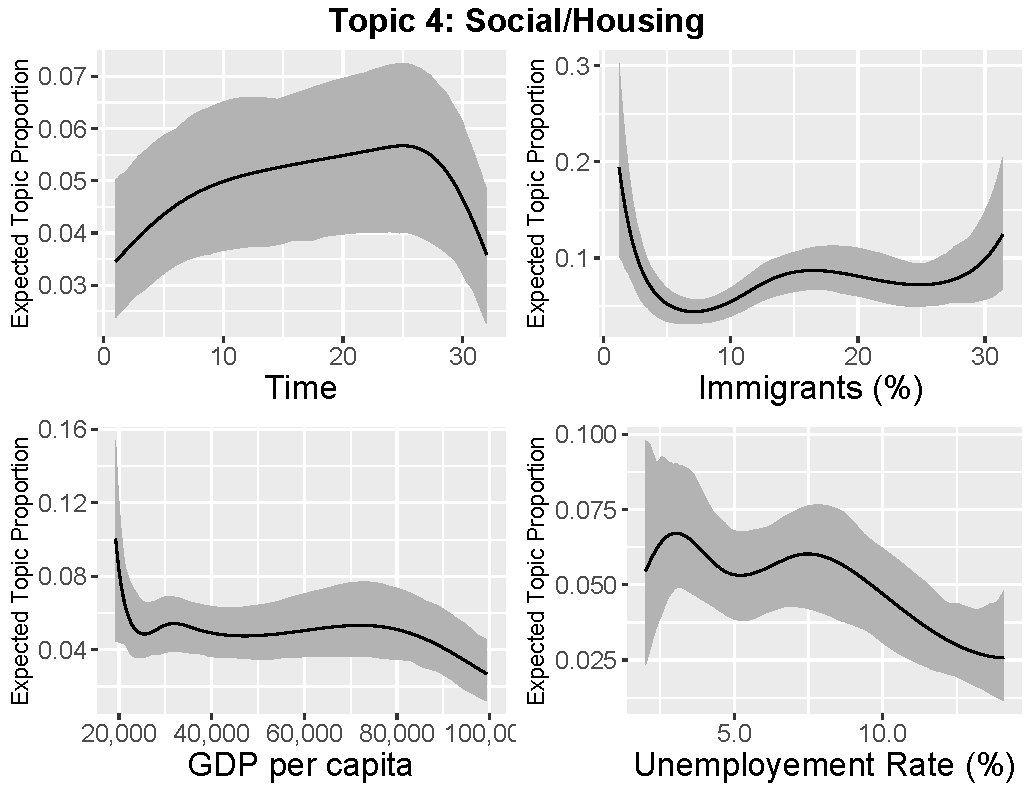
\includegraphics[width=\linewidth]{4_6/quasi_t4_cont_ctm.pdf}
  \end{subfigure}
  \begin{subfigure}[b]{0.4\linewidth}
    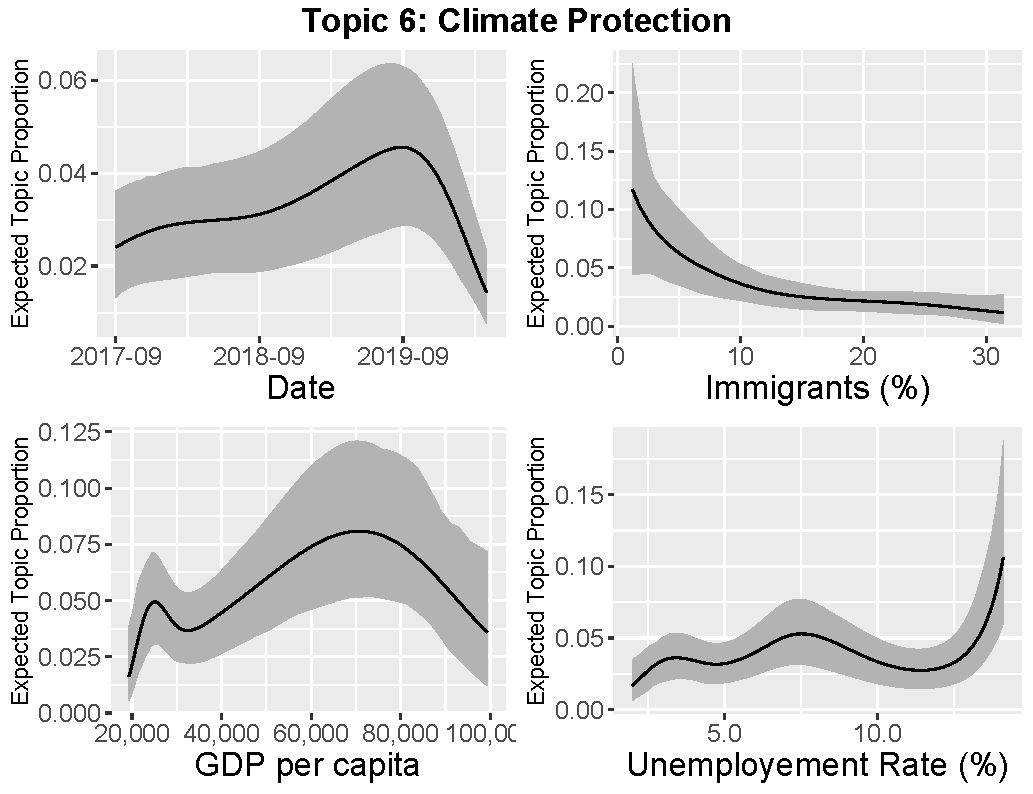
\includegraphics[width=\linewidth]{4_6/quasi_t6_cont_ctm.pdf}
  \end{subfigure}
  \caption{Mean and 95\% credible intervals for smooth effects, obtained
using a quasibinomial GLM (no covariates included in model estimation).}
  \label{fig:quasi_t46_cont_ctm}
\end{figure}

\begin{figure}[h!]
  \centering
  \captionsetup{justification=centering,margin=2cm}
  \begin{subfigure}[b]{0.4\linewidth}
    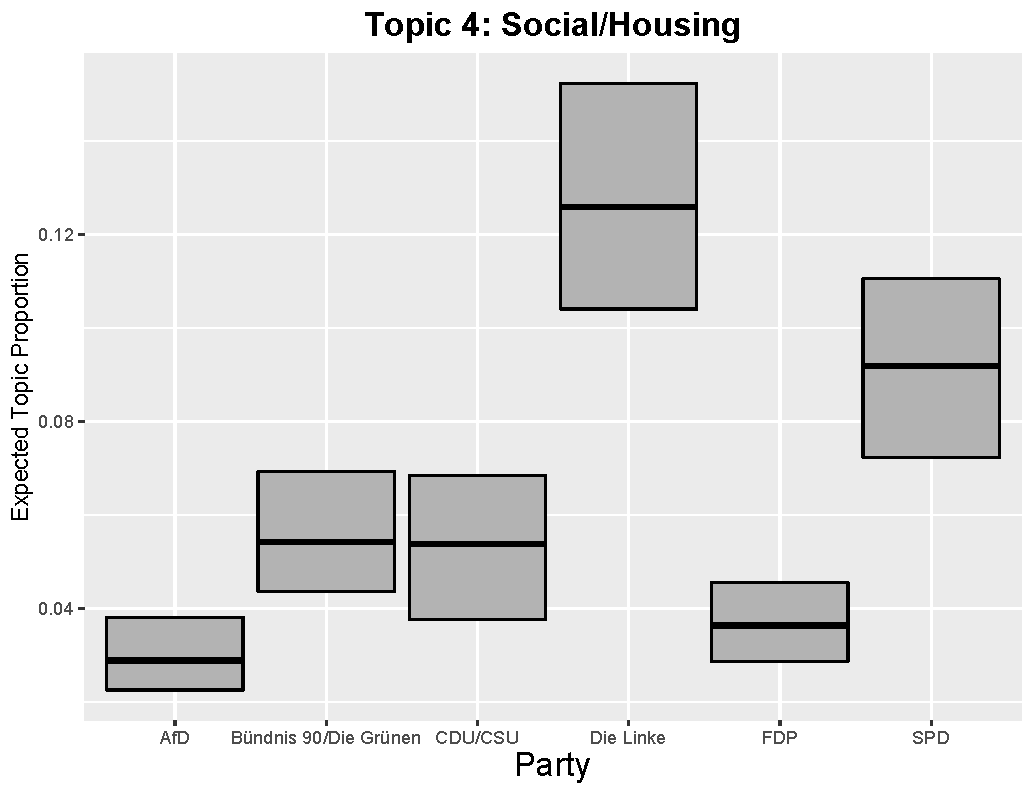
\includegraphics[width=\linewidth]{4_6/quasi_t4_cat_ctm.pdf}
  \end{subfigure}
  \begin{subfigure}[b]{0.4\linewidth}
    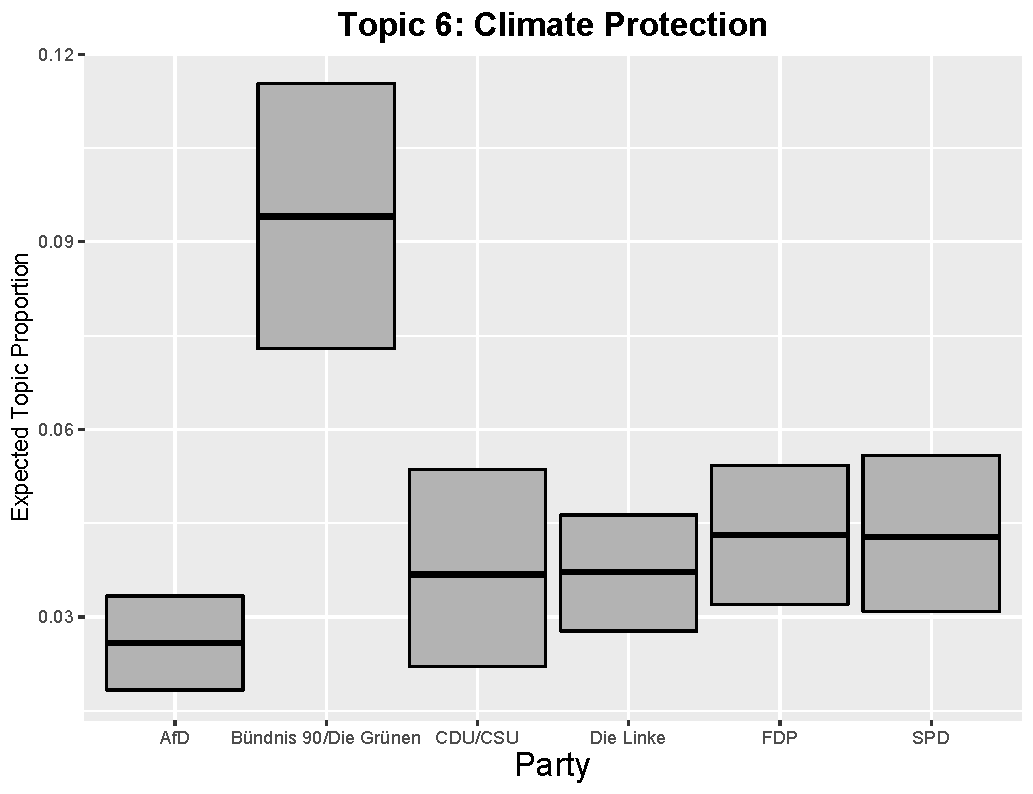
\includegraphics[width=\linewidth]{4_6/quasi_t6_cat_ctm.pdf}
  \end{subfigure}
  \caption{Mean and 95\% credible intervals for different political parties,
obtained using a quasibinomial GLM (no covariates included in model estimation).}
  \label{fig:quasi_t46_cat_ctm}
\end{figure}

Topic proportions across parties for topics 3, 6, and 1 (Right/Nationalist) are further summarized in the plot below. Comparing the results to those of the STM for the additional topic 1, a rather large difference can be seen: the overall topic proportion for the AfD party is now almost 10\% lower than in the STM (though still at almost 35\%). Furthermore, for all topics and covariates, the comparison between STM and CTM does not change if we use beta regression instead of quasibinomial regression within the method of composition, corroborating our results (see appendix XXX).

\begin{figure}[h!]
  \centering
  \captionsetup{justification=centering,margin=2cm}
  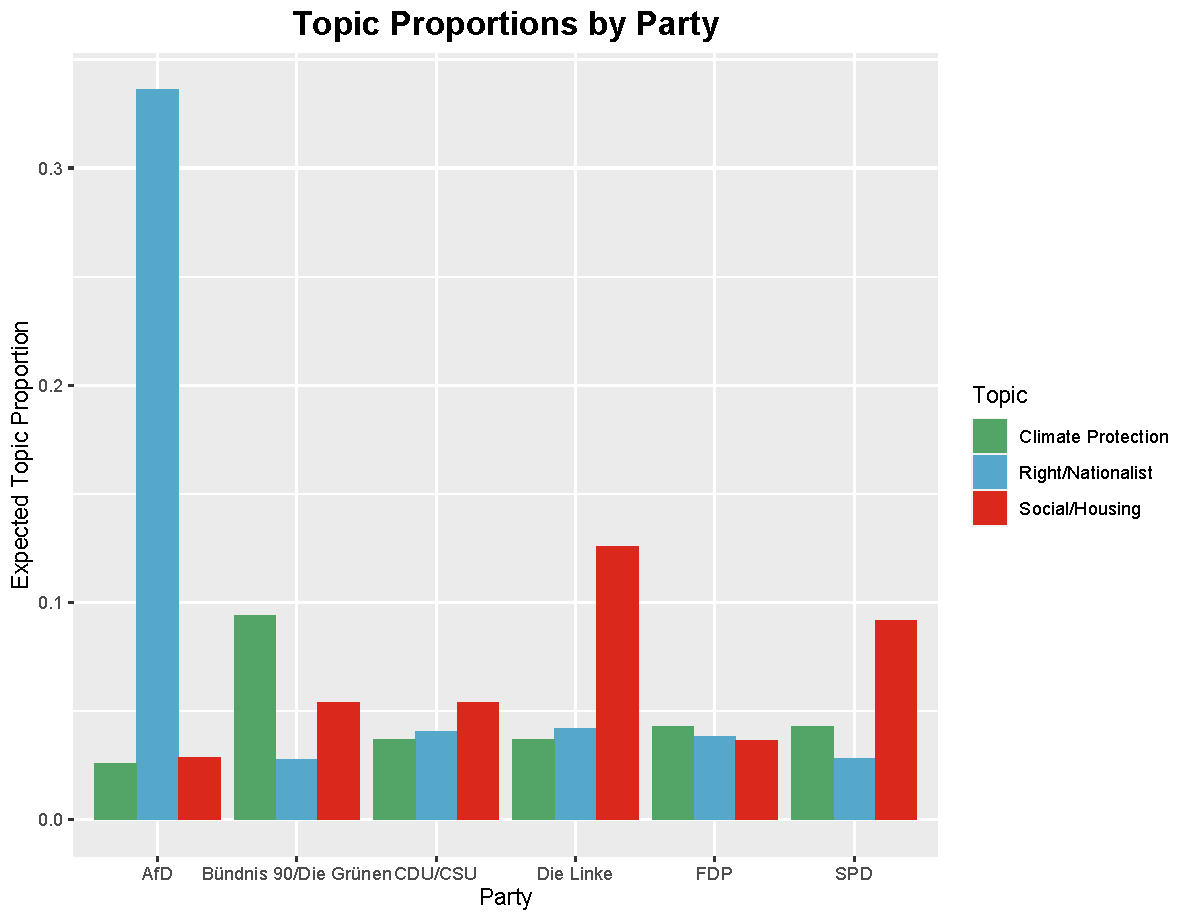
\includegraphics[width=\linewidth]{4_6/quasi_t146_cat_ctm.pdf}
  \caption{Mean and 95\% credible intervals for different political parties,
obtained using a quasibinomial GLM (no covariates included in model estimation).}
  \label{fig:quasi_t146_cat_ctm}
\end{figure}

All in all, the relationships between topical prevalence variables and topic proportions are very similar to those of the STM when instead using a clean 2-step estimation procedure where no covariate information is used in the model estimation. This indicates that the problem of double usage of covariate information in the STM, potentially leading to overfitting, is not overly severe.


\bibliography{bibliography}
\bibliographystyle{plainnat}

\end{document}
\section{Train-test Split}

In our analyses from section 4.4, we first estimated the latent topic proportions using the stm, and then assessed the relation between these document-level topic proportions and prevalence covariates. In particular, the documents that were used to obtain the topic proportions were the same that were subsequently used to quantify relationships between covariates and topic proportions. As \cite{egami2018make} argue, this double usage of data is a form of overfitting and hence inferences about covariate effects are biased. Additionally, since in the stm prevalence covariates affect estimated topic proportions, there is not only a mere double usage of data (i.e., in the sense that the same documents are used twice), but also a direct double usage of prevalence covariates, as the estimated latent topic proportions are regressed on the former.

Both problems can be addressed using the framework proposed by \cite{egami2018make}. The general idea is to split the data $\mathcal{D}$ into a training set $\mathcal{D}_{\text{train}}$ and a test set $\mathcal{D}_{\text{test}}$, and utilize the training set in order to determine a model to infer latent topic proportions from any text assumed to be generated by the same underlying process as the training set. Subsequently, this estimated model is applied on the test set, in order to assess the relation between test set topic proportions and test set prevalence covariates. In the following, we will explain the exact procedure for the stm (note that \cite{egami2018make} focus, for the most part, on the general framework, while the exact application within the stm is not discussed in-depth) and evaluate the results when applied to our data. 

\subsection{Model Estimation on the Training Set}

On the training set, we estimate components of the stm similarly to the estimation on the full data set. That is, we input documents, i.e., words and metadata from the training set, and obtain estimates $(\hat{\beta}_{\text{train}}, \hat{\Gamma}_{\text{train}}, \hat{\Sigma}_{\text{train}})$, where $\hat{\beta}_{\text{train}}$ is associated with the topic-word distribution, and $\hat{\Gamma}_{\text{train}}$ as well as $\hat{\Sigma}_{\text{train}}$ are the topical prevalence parameters. 

\subsection{Prediction of Topic Proportions on the Test Set}

Prediction of the topic proportions on the test is not straightforward, since the topic proportions are latent and the stm is not built for the purpose of predicting these latent variables on a set of new, unseen data. The fundamental idea is to estimate the variational posterior of the latent variables, that is, the topic proportions $\theta_d$, where $d \in \mathcal{D}_{\text{test}}$ (note that $z_d$ is integrated out in the stm), conditioned on the model parameters $(\hat{\beta}_{\text{train}}, \hat{\Gamma}_{\text{train}}, \hat{\Sigma}_{\text{train}})$, as well as the words $W_{\text{test}}$ from the test set. This functionality is implemented in the \textit{stm} package through the function \textit{fitNewDocuments}, which per default outputs the MAP estimates of topic proportions $\theta_d$, for all $d \in \mathcal{D}_{\text{test}}$. Note that estimating the variational posterior of the latent variables, conditioned on the parameters and the words, is precisesly what occurs during each E-step of the EM Algorithm. Thus, the implementation of \textit{fitNewDocuments} simply consists of one E-step with inputs $(\hat{\beta}_{\text{train}}, \hat{\Gamma}_{\text{train}}, \hat{\Sigma}_{\text{train}}, W_{\text{test}})$. It is, however, not obvious how to exactly input $\hat{\Gamma}_{\text{train}}$ and  $\hat{\Sigma}_{\text{train}}$ into the E-step. Depending on the characteristics of the specific analysis conducted by the researcher, \cite{egami2018make} propose three different alternatives:
\begin{enumerate}
\item \textbf{Covariate-specific prior}: Before applying the E-step, $\hat{\Gamma}_{\text{train}}$ is used to obtain $\hat{\mu}_d := (\hat{\Gamma}_{\text{train}})^T(x_d)^T$, for each document $d \in \mathcal{D}_{\text{test}}$ in the test set. Each document is then updated performing the E-step with inputs $({\mu}_d, \Sigma) = (\hat{\mu}_d, \hat{\Sigma}_{\text{train}})$ together with the respective document specific words as well as $\hat{\beta}_{\text{train}}$ (for the exact update machanism see pp. 992-993, \cite{roberts2013structural}). The problem with this approach is, however, that for two documents from the test set containaing the exact same words, different topic proportions are predicted if the prevalence covariates differ. However, in such a case we would want the causal effect of the covariates on the topic proportions to be zero.
\item \textbf{Average prior}: The average prior circumvents the above described problem of the covariate-specific prior by simply using - for each document in the test set - the average $\overline{\mu}_{\text{train}} := \frac{1}{|\mathcal{D}_{\text{train}}|}\sum_{d \in \mathcal{D}_{\text{train}}} (\hat{\Gamma}_{\text{train}})^T(x_d)^T$ of all document-specific means from the training set. The covariance $\hat{\Sigma}_{\text{train}}$ is recalculated based on the new average $\overline{\mu}_{\text{train}}$ according to formula (11) on p.\ 993, \cite{roberts2013structural}. In this scenario, prevalence covariates from the test have no influence at all on the predicted topic proportions. 
\item \textbf{No prior}: If no prior is used, then for each document $d \in \mathcal{D}_{\text{test}}$ in the test set the E-step is performed using $\mu_d=0$ and replacing $\hat{\Sigma}_{\text{train}}$ with a diagonal covariance matrix with very large diagonals.
\end{enumerate}

The covariate-specific prior can not be used in our case due to the above described problem, that different topic proportions are predicted for identically worded test set documents, if their prevalence covariates differ. The option "no prior" can be useful if the metadata on the test set is believed to be linked differently to topics than is the case on the training set. In most cases the second option, "average prior", should provide the best trade-off, since in this case metadata from the training set is directly used to predict topic proportions, but the problem of the covariate-specific prior is solved. Note that hence in this case there is no double usage of covariates.

\subsection{Results}

We now depict the results obtained conducting a train-test split, where we split the data into two equally sized sets, and choose the option "average prior".
\section{Conclusion}

TBD
\newpage
\section{Appendix 1}

In line with \cite{wang2013variational}, consider a generic topic model with latent variables $\theta$ and $z$ as well as observed data $x$:
\begin{align*}
p(\theta,z,x) &= p(x|z)p(z|\theta)p(\theta).
\end{align*}
The exact posterior distribution
\begin{align*}
p(\theta,z|x) &= \frac{p(\theta,z,x)}{\int p(\theta,z,x)dzd\theta}
\end{align*}
is usually intractable due to the high-dimensional integral, which is why the distribution needs to be approximated.

As stated in section 2.3, in variational inference a simple distribution family $q(\theta,z)$ is posited and subsequently, we determine the member of this family - that is, the variational parameter(s) - that minimizes the KL divergence. Note that, for computational purposes, we compute KL divergence of the true posterior $p$ from the approximating posterior $q$, $KL(q||p)$, whereas intuitively one would seek to minimize $KL(p||q)$.

The most popular variational inference technique is mean-field variational inference (also: mean-field variational Bayes), where we posit full factorizability of $q(\theta,z)$: $q(\theta,z) = q(\theta)q(z)$. That is, $\theta$ and $z$ are assumed to be independent with their own distributions and variational parameters $\phi$ (which we suppress for improved readability). Since $\theta$ and $z$ are actually dependent, this approximate distribution family $q(\theta,z)$ does not contain the true posterior $p(\theta,z|x)$.  

Let us now write out the KL divergence of $p$ from $q$:
\begin{align*}
KL(q||p) &= \mathbb{E}_q[\log\frac{q(\theta,z)}{p(\theta,z|x)}] \\
&= \mathbb{E}_q[\log(q(\theta,z))] - \mathbb{E}_q[\log(p(\theta,z|x))] \\
&=\mathbb{E}_q[\log(q(\theta,z))] - \mathbb{E}_q[\log(p(\theta,z,x))] + \log(p(x)) 
\end{align*}
Since $KL(q||p) \geq 0$ (which can be easily shown using Jensen's inequality), it follows that:
\begin{align*}
\log(p(x)) & \geq \mathbb{E}_q[\log(p(\theta,z,x))] - \mathbb{E}_q[\log(q(\theta,z))].
\end{align*}
The left-hand side of the above inequality is the marginal log likelihood of observed data $x$ and is also called evidence (of the observed data). Note that the evidence is not computable - otherwise we would not need to resort to variational inference in the first place. The right-hand side thus presents a lower bound on the evidence and we define the \textit{Evidence Lower BOund} (ELBO) as:
\begin{align*}
ELBO := \mathbb{E}_q[\log(p(\theta,z,x))] - \mathbb{E}_q[\log(q(\theta,z))],
\end{align*}
where the second component of the ELBO, $\mathbb{E}_q[\log(q(\theta,z))$, is the entropy of the approximate distribution $q$. Equivalently, we could say that the evidence constitutes an upper bound for the ELBO. This means that we actively maximize the ELBO (which is therefore also called \textit{variational objective}), which in turn is equivalent to minimizing the KL divergence of the true posterior $p(\theta,z|x)$ from the approximate distribution $q(\theta,z)$. Therefore, the approximation $q(\theta,z)$ - or, more precisely, the variational parameters $\phi$ of $q(\theta)$ and $q(z)$ - that maximizes the ELBO simultaneously minimizes KL divergence (\citealp{blei2003latent, wang2013variational}). \cite{wang2013variational} show that for the chosen factorization of the joint distribution $p(\theta,z,x)$, and using the optimality conditions as derived in \cite{bishop2006pattern}, we obtain the following solutions when setting $\frac{\partial ELBO}{\partial q}\overset{!}{=}0$:
\begin{align*}
q^{*}(\theta) \propto exp\{\mathbb{E}_{q(z)}[\log(p(z|\theta))p(\theta)]\}, \\
q^{*}(z) \propto exp\{\mathbb{E}_{q(\theta)}[\log(p(x|z))p(z|\theta)]\}.
\end{align*}
The coordinate ascent algorithm iteratively updates one of these two expressions while holding the other one constant, but requires closed-form updates to do so. This requirement is fulfilled as long as all model nodes are conditionally conjugate, i.e., as long as for each node in the model "its conditional distribution given its Markov blanket (i.e., the set of random variables that it is dependent on in the posterior) is in the same family as its conditional distribution given its parents (i.e., its factor in the joint distribution)" (\cite{wang2013variational}, p.\ 1008). The authors consequently define a class of models where some nodes are not conditionally conjugate, the so-called \textit{nonconjugate models}; for this class, using Laplace approximations, the variational family is shown to be $q(\theta,z) = q(\theta|\mu,\Sigma)q(z|\phi)$; that is, $q(\theta)$ is now Gaussian with variational parameters $\mu$ and $\Sigma$.

The STM in particular constitutes a nonconjugate model, since $p(\theta)$ is logistic normal and thus not conjugate with respect to the multinomial distribution $p(z|\theta)$. Consequently, no closed-form update is available for $q(\eta)$. Using mean-field variational inference, the approximate posterior family is $\prod_{d=1}^{D}q(\eta_d)q(z_d)$, where $q(\eta_d)$ is Gaussian and $q(z)$ is binomial (\citealp{roberts2016model}). Given the posterior, inference now consists in finding the particular member of the posterior distribution family that maximizes the approximate ELBO. (Due to the subsequent Laplace approximation, ELBO does not constitute a true lower bound on the evidence and the updates do not maximize ELBO directly, which is why \cite{roberts2013structural} use the term \textit{approximate} ELBO. See \cite{wang2013variational} for further discussion.) Applying Laplace variational inference, we approximate $q(\eta_d)$ using a (quadratic) Taylor expression around the maximum-a-posteriori (MAP) estimate $\hat{\eta}_d$, which yields a Gaussian variational posterior $q(\eta_d)$, centered around $\hat{\eta}_d$, and allows for a closed-form solution of $q(z_d)$. Iteratively updating $q(\eta_d)$ and $q(z_d)$ thus constitutes the E-step of the EM algorithm.

The M-step consists in maximizing the approximate ELBO with respect to model parameters. Prevalence parameters $\Gamma$ and $\Sigma$ are updated through linear regression and maximum likelihood estimation (MLE), respectively. The updates for topic-word distributions $\beta_k$ (or $\beta_{k,a}$ if a content covariate is specified) are obtained through multinomial logistic regression. Further details are provided in \cite{roberts2013structural} and in the appendix of \cite{roberts2013structural}. Moreover, the appendix of \cite{blei2003latent} provides a detailed description of variatonal inference and empirical parameter estimation for the (conditionally conjugate) LDA model.

\section{Appendix 2}

\noindent
\textit{Topic 1 Top Words:}\\
 	 \textbf{Highest Prob:} buerg, link, merkel, frau, sich \\
 	 \textbf{FREX:} altpartei, islam, linksextremist, asylbewerb, linksextrem \\
 	 \textbf{Lift:} eitan, 22jaehrig, abdelsamad, abgehalftert, afdforder \\
 	 \textbf{Score:} altpartei, linksextremist, frauenkongress, islamist, boehring \\
\textit{Topic 2 Top Words:}\\
 	 \textbf{Highest Prob:} frag, einfach, find, genau, halt \\
 	 \textbf{FREX:} geles, tweet, sorry, quatsch, lustig \\
 	 \textbf{Lift:} baseball, demjen, duitsland, garn, haeh \\
 	 \textbf{Score:} schmunzel, tweet, fuerstenberg, sorry, geles \\
\textit{Topic 3 Top Words:}\\
 	 \textbf{Highest Prob:} brauch, wichtig, leid, dank, klar \\
 	 \textbf{FREX:} emissionshandel, soli, marktwirtschaft, feedback, co2steu \\
 	 \textbf{Lift:} aequivalenz, altersvorsorgeprodukt, bildungsqualitaet, co2limit, co2meng \\
 	 \textbf{Score:} emissionshandel, co2limit, basisrent, euet, technologieoff \\
\textit{Topic 4 Top Words:}\\
 	 \textbf{Highest Prob:} sozial, miet, kind, arbeit, brauch \\
 	 \textbf{FREX:} mindestlohn, miet, wohnungsbau, mieterinn, loehn \\
 	 \textbf{Lift:} auseinanderfaellt, baugipfel, bestandsmiet, billigflieg, binnennachfrag \\
 	 \textbf{Score:} miet, mieterinn, mietendeckel, grundsicher, bezahlbar \\
\textit{Topic 5 Top Words:}\\
 	 \textbf{Highest Prob:} digital, jung, duesseldorf, bildung, christian \\
 	 \textbf{FREX:} fdpbundestagsabgeordnet, duesseldorf, rimkus, intelligenz, startups \\
 	 \textbf{Lift:} boeing, dettenheim, duesseldorfbilk, eheim, elektrokleinstfahrzeug \\
 	 \textbf{Score:} fdpbundestagsabgeordnet, rimkus, digital, duesseldorf, uranfabr \\
\textit{Topic 6 Top Words:}\\
 	 \textbf{Highest Prob:} gruen, klimaschutz, brauch, klar, euro \\
 	 \textbf{FREX:} fossil, erneuerbar, kohleausstieg, verkehrsminist, verkehrsw \\
 	 \textbf{Lift:} abgasbetrug, abgebaggert, abschalteinricht, abschaltet, ammoniak \\
 	 \textbf{Score:} erneuerbar, fossil, zdebel, verkehrsminist, klimaschutz \\
\textit{Topic 7 Top Words:}\\
 	 \textbf{Highest Prob:} europaeisch, wichtig, europa, international, thank \\
 	 \textbf{FREX:} foreign, policy, clos, clear, important \\
 	 \textbf{Lift:} alam, bucerius, bulgaria, doping, judgment \\
 	 \textbf{Score:} need, important, great, foreign, today \\
\textit{Topic 8 Top Words:}\\
 	 \textbf{Highest Prob:} kris, wichtig, brauch, kind, hilf \\
 	 \textbf{FREX:} corona, coronakris, virus, pandemi, coronavirus \\
 	 \textbf{Lift:} covid19, schutzmask, 600milliardenfond, abiturpruef, abstandhalt \\
 	 \textbf{Score:} corona, coronakris, pandemi, coronavirus, virus \\
\textit{Topic 9 Top Words:}\\
 	 \textbf{Highest Prob:} krieg, link, europaeisch, regier, international \\
 	 \textbf{FREX:} milita, voelkerrechtswidr, aufruest, waffenexport, libysch \\
 	 \textbf{Lift:} katalan, abho, airbas, antimilitarist, aufklaerungsdat \\
 	 \textbf{Score:} voelkerrechtswidr, libysch, milita, iran, voelkerrecht \\
\textit{Topic 10 Top Words:}\\
 	 \textbf{Highest Prob:} herzlich, glueckwunsch, wichtig, freu, gespraech \\
 	 \textbf{FREX:} gmuend, achim, backnang, sommertour, schwaebisch \\
 	 \textbf{Lift:} 24stundendien, abschlussfoto, absolventinn, abstandskriteri, afrikastrategi \\
 	 \textbf{Score:} backnang, gmuend, achim, bentheim, sauerla \\
\textit{Topic 11 Top Words:}\\
 	 \textbf{Highest Prob:} pfleg, versorg, wichtig, chemnitz, patient \\
 	 \textbf{FREX:} mention, neuwied, automatically, unfollowed, checked \\
 	 \textbf{Lift:} mention, unfollowed, alicia, alois.karl, altenkirch \\
 	 \textbf{Score:} mention, unfollowed, reach, automatically, windhag \\
\textit{Topic 12 Top Words:}\\
 	 \textbf{Highest Prob:} frau, gruen, frag, antrag, debatt \\
 	 \textbf{FREX:} bielefeld, innenausschuss, streichung, selbstbestimm, bundesinnenminist \\
 	 \textbf{Lift:} abstammungsrecht, altruist, atrium, bundesgeschaeftsstell, cannabispolit \\
 	 \textbf{Score:} bielefeld, innenausschuss, u.spd, lobbyistengab, amri \\
\textit{Topic 13 Top Words:}\\
 	 \textbf{Highest Prob:} berlin, schoen, dank, freu, woch \\
 	 \textbf{FREX:} buongiorno, moin, frank, kiel, leipzig \\
 	 \textbf{Lift:} altlandsberg, anrath, bergenenkheim, blindenleitsyst, bueromitarbeit \\
 	 \textbf{Score:} buongiorno, moin, schoen, neers, berlin \\
\textit{Topic 14 Top Words:}\\
 	 \textbf{Highest Prob:} partei, link, demokrat, klar, wahl \\
 	 \textbf{FREX:} thuering, hoeck, faschist, neuwahl, kemmerich \\
 	 \textbf{Lift:} epost, gezittert, oktoberrevolution, parteischaed, uebergangsmp \\
 	 \textbf{Score:} faschist, kemmerich, thuering, ramelow, hoeck \\
\textit{Topic 15 Top Words:}\\
 	 \textbf{Highest Prob:} dank, glueckwunsch, herzlich, gemeinsam, europa \\
 	 \textbf{FREX:} zusammenhalt, antisemitismus, lasst, hass, vielfalt \\
 	 \textbf{Lift:} 40jahr, afdtyp, dierk, fruendt, mutmacherinn \\
 	 \textbf{Score:} dank, hass, zusammenhalt, binding, antisemitismus \\


\subsection*{Plots of section 4.4}

\begin{figure}[h!]
  \centering
  \begin{subfigure}[b]{0.4\linewidth}
    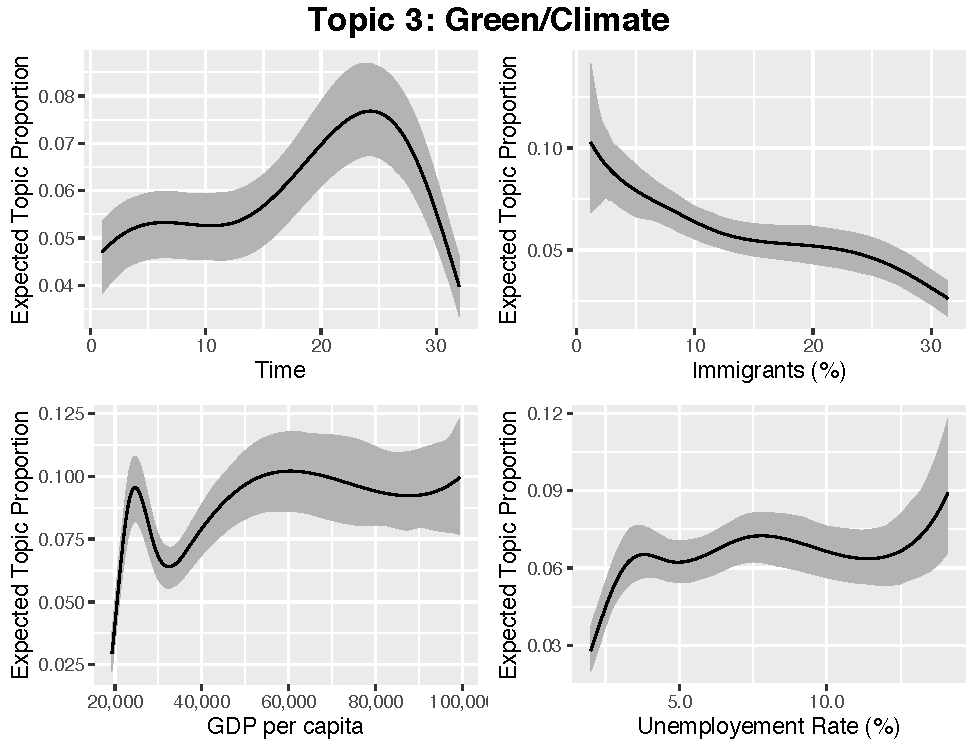
\includegraphics[width=\linewidth]{../plots/appendix/4_4/beta_t3_cont.pdf}
  \end{subfigure}
  \begin{subfigure}[b]{0.4\linewidth}
    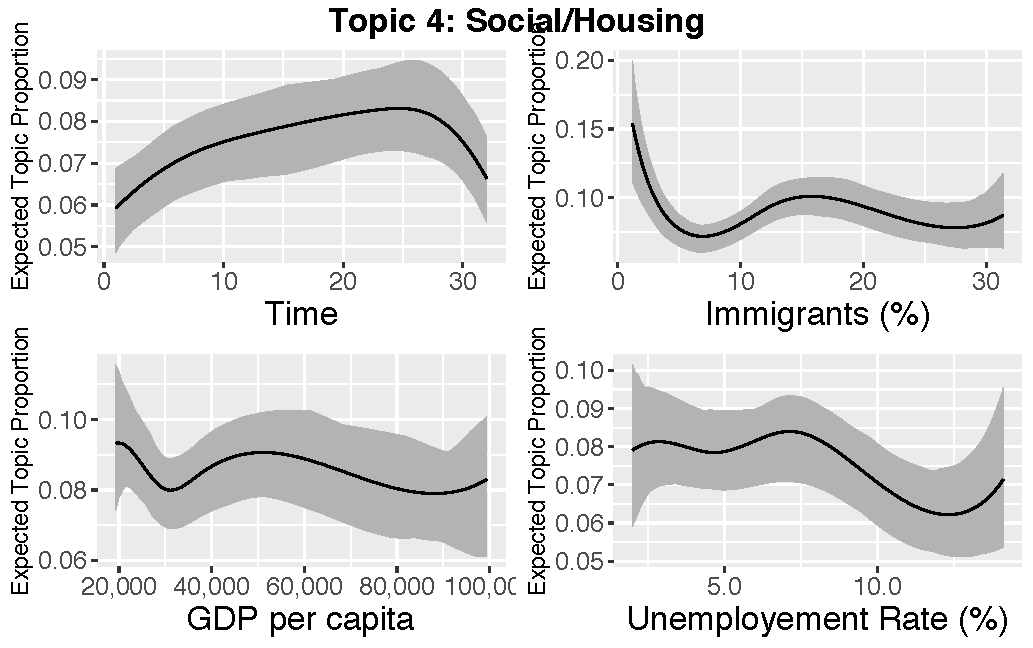
\includegraphics[width=\linewidth]{../plots/appendix/4_4/beta_t4_cont.pdf}
  \end{subfigure}
  \caption{bla}
  \label{fig:coffee}
\end{figure}

\begin{figure}[h!]
  \centering
  \begin{subfigure}[b]{0.4\linewidth}
    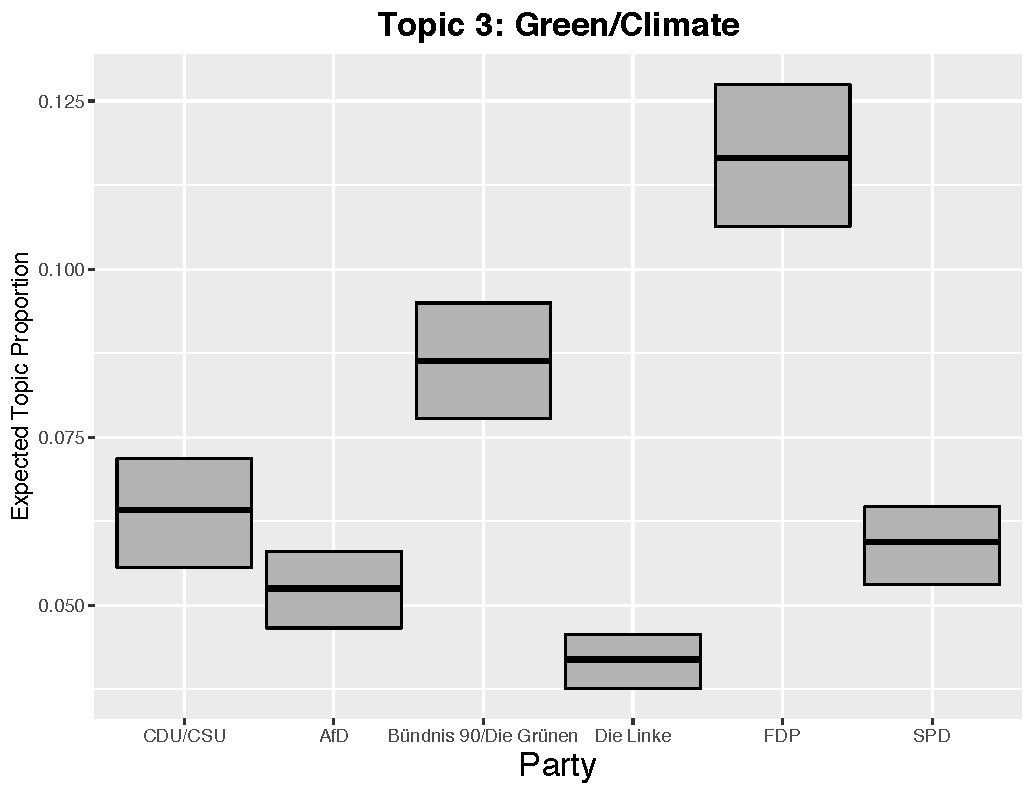
\includegraphics[width=\linewidth]{../plots/appendix/4_4/beta_t3_cat.pdf}
  \end{subfigure}
  \begin{subfigure}[b]{0.4\linewidth}
    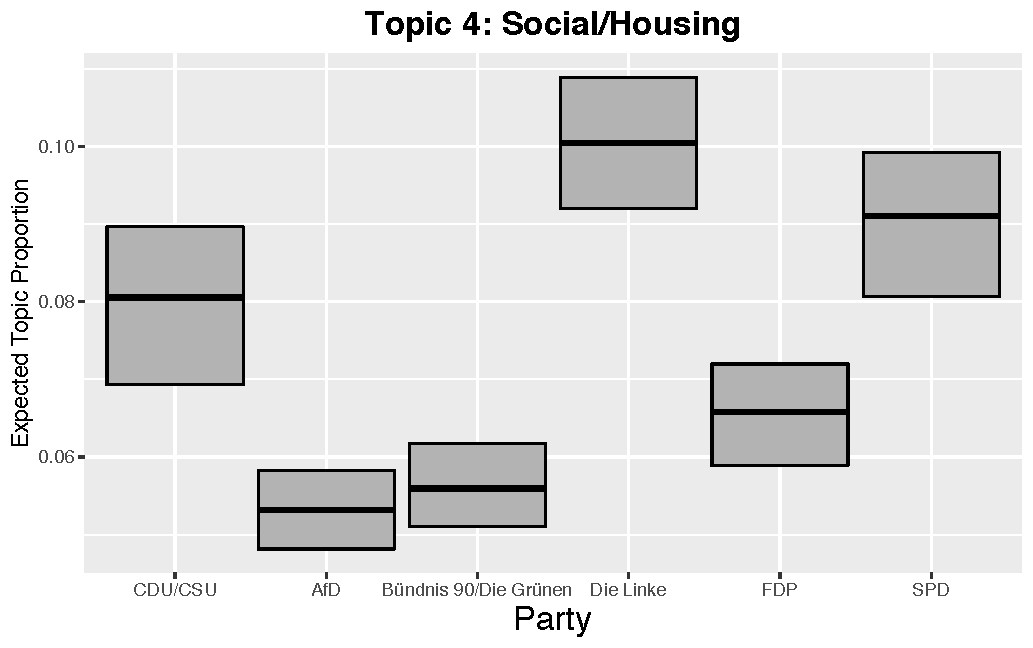
\includegraphics[width=\linewidth]{../plots/appendix/4_4/beta_t4_cat.pdf}
  \end{subfigure}
  \caption{blabla}
  \label{fig:coffee}
\end{figure}

\begin{figure}[h!]
  \centering
  \captionsetup{justification=centering,margin=2cm}
  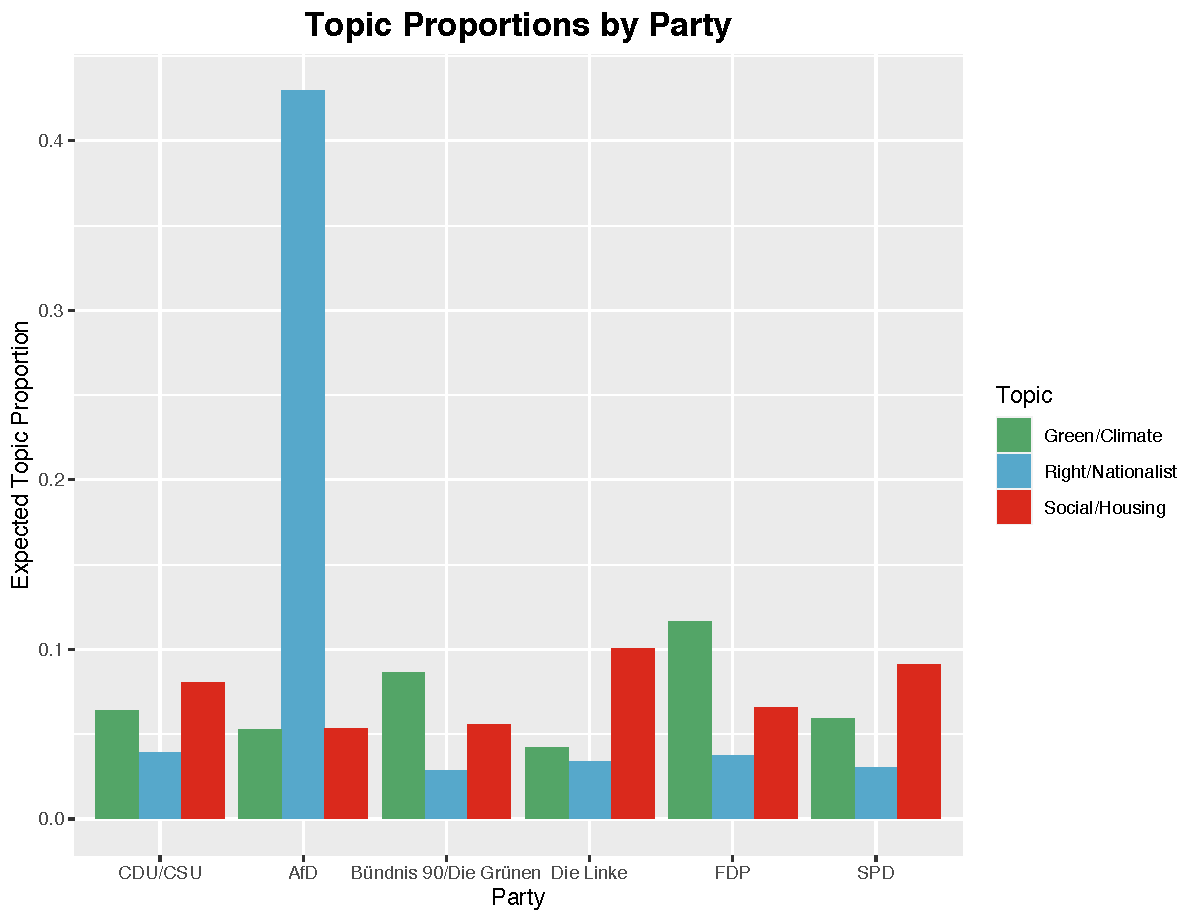
\includegraphics[scale = 0.5]{../plots/appendix/4_4/beta_t134_cat.pdf}
  \caption{Topical prevalence by political party for topics 1, 2, and 3.}
  \label{fig:boat1}
\end{figure}

\begin{figure}[h!]
    \centering
  \begin{subfigure}[b]{0.3\linewidth}
    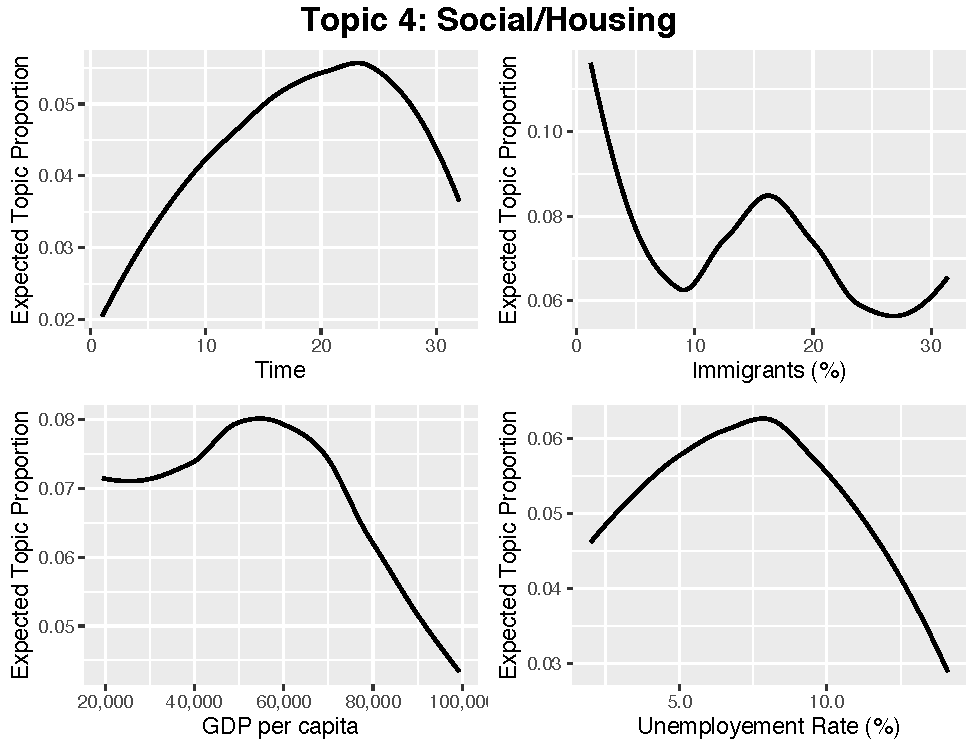
\includegraphics[width=\linewidth]{../plots/appendix/4_4/direct_t4_without_credible.pdf}
  \end{subfigure}
  \begin{subfigure}[b]{0.3\linewidth}
    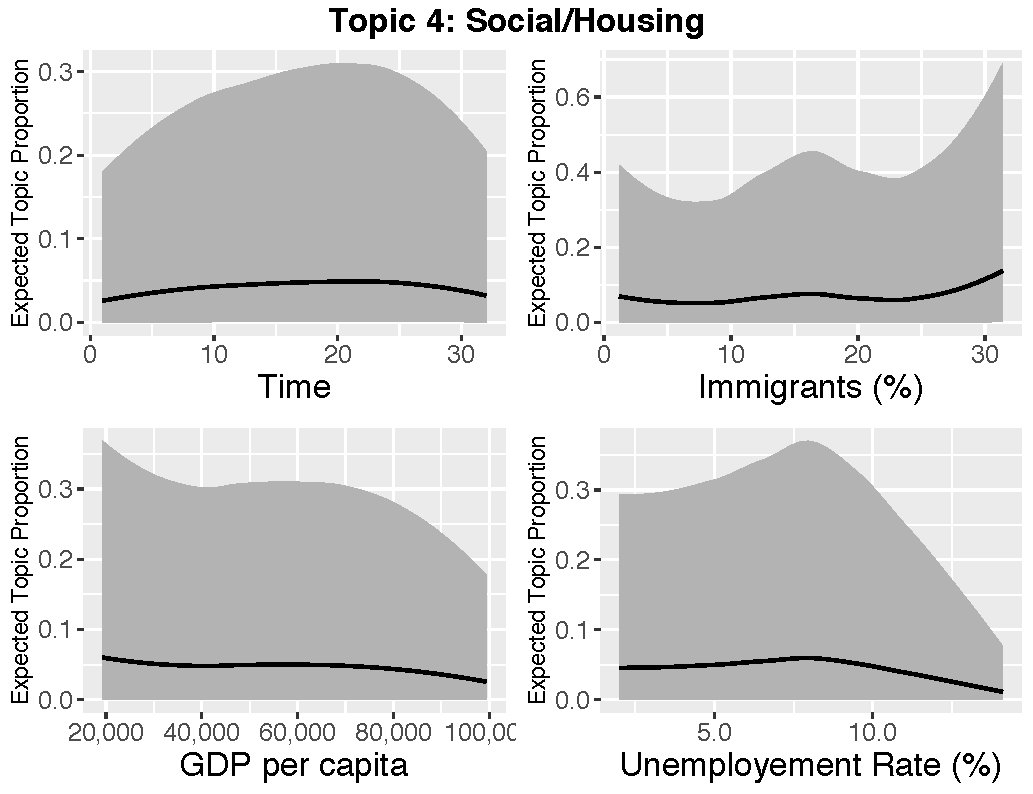
\includegraphics[width=\linewidth]{../plots/appendix/4_4/direct_t4_with_credible.pdf}
  \end{subfigure}
  \begin{subfigure}[b]{0.3\linewidth}
    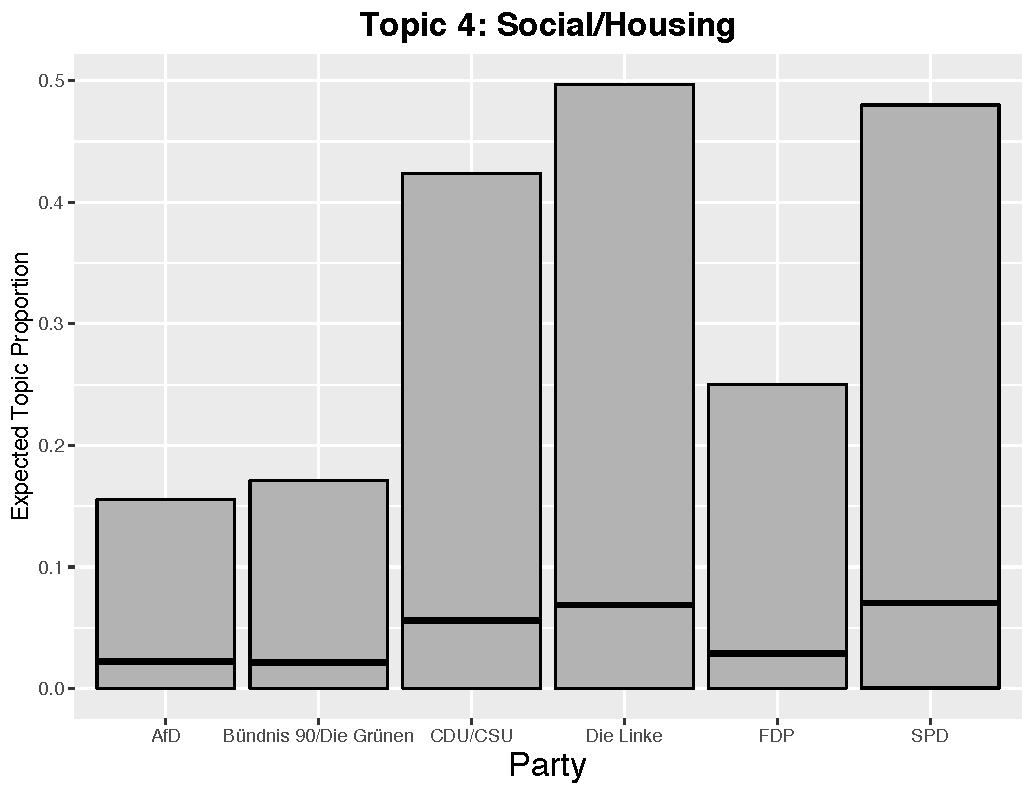
\includegraphics[width=\linewidth]{../plots/appendix/4_4/direct_t4_cat.pdf}
  \end{subfigure}
  \caption{bla}
  \label{fig:coffee}
\end{figure}


\subsection*{Plots of section 4.6}

\begin{figure}[h!]
  \centering
  \begin{subfigure}[b]{0.4\linewidth}
    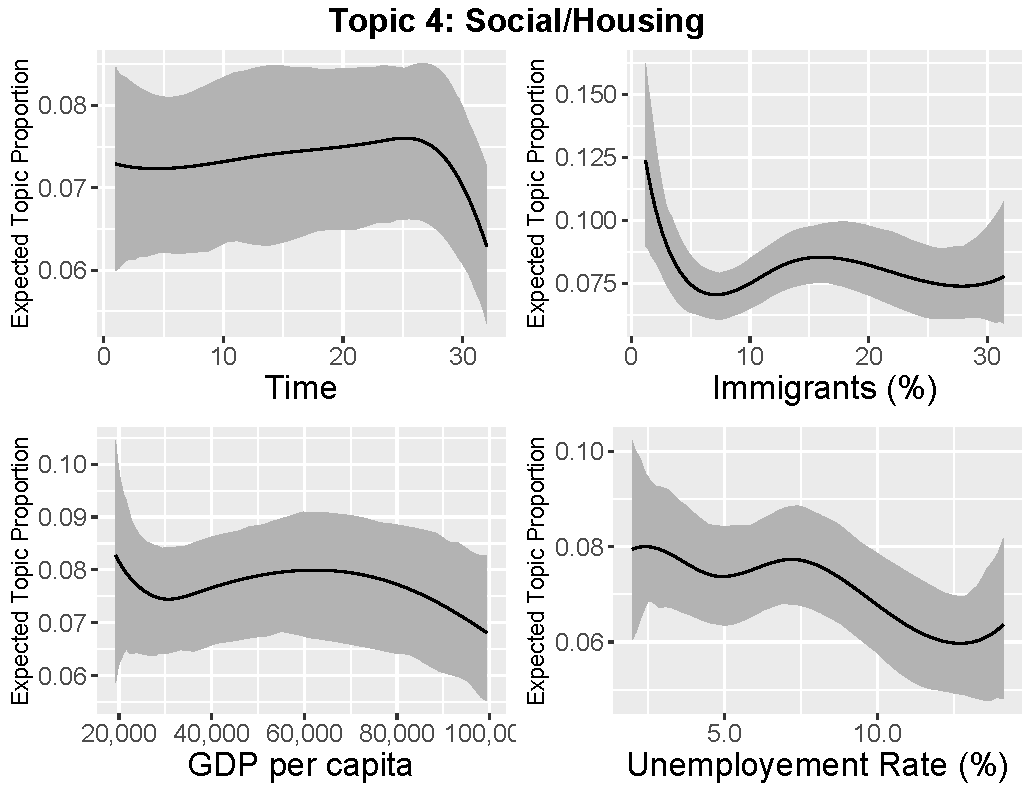
\includegraphics[width=\linewidth]{../plots/appendix/4_6/beta_t4_cont_ctm.pdf}
  \end{subfigure}
  \begin{subfigure}[b]{0.4\linewidth}
    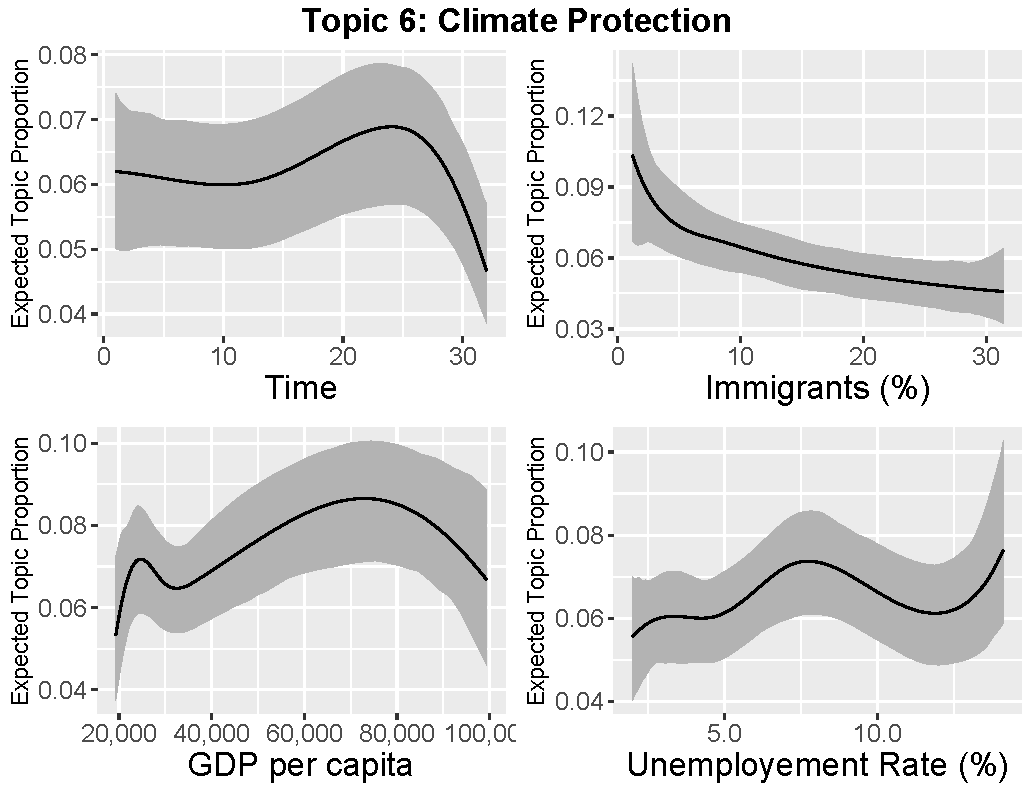
\includegraphics[width=\linewidth]{../plots/appendix/4_6/beta_t6_cont_ctm.pdf}
  \end{subfigure}
  \caption{bla}
  \label{fig:beta_t46_cont_ctm}
\end{figure}

\begin{figure}[h!]
  \centering
  \begin{subfigure}[b]{0.4\linewidth}
    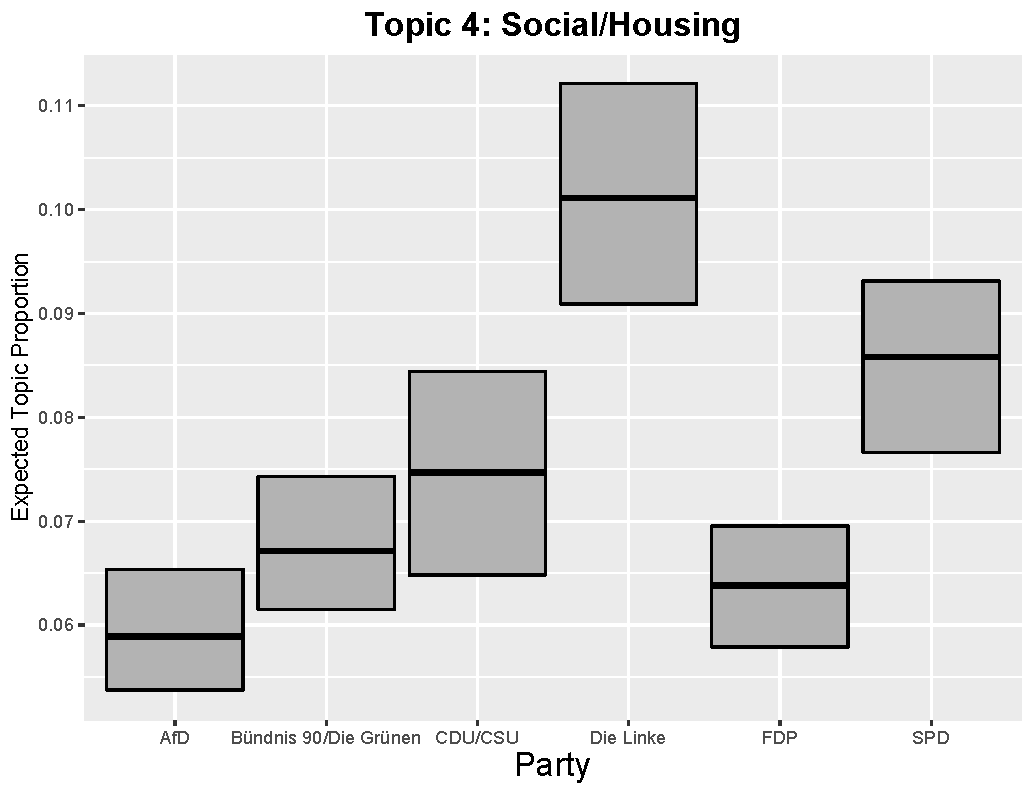
\includegraphics[width=\linewidth]{../plots/appendix/4_6/beta_t4_cat_ctm.pdf}
  \end{subfigure}
  \begin{subfigure}[b]{0.4\linewidth}
    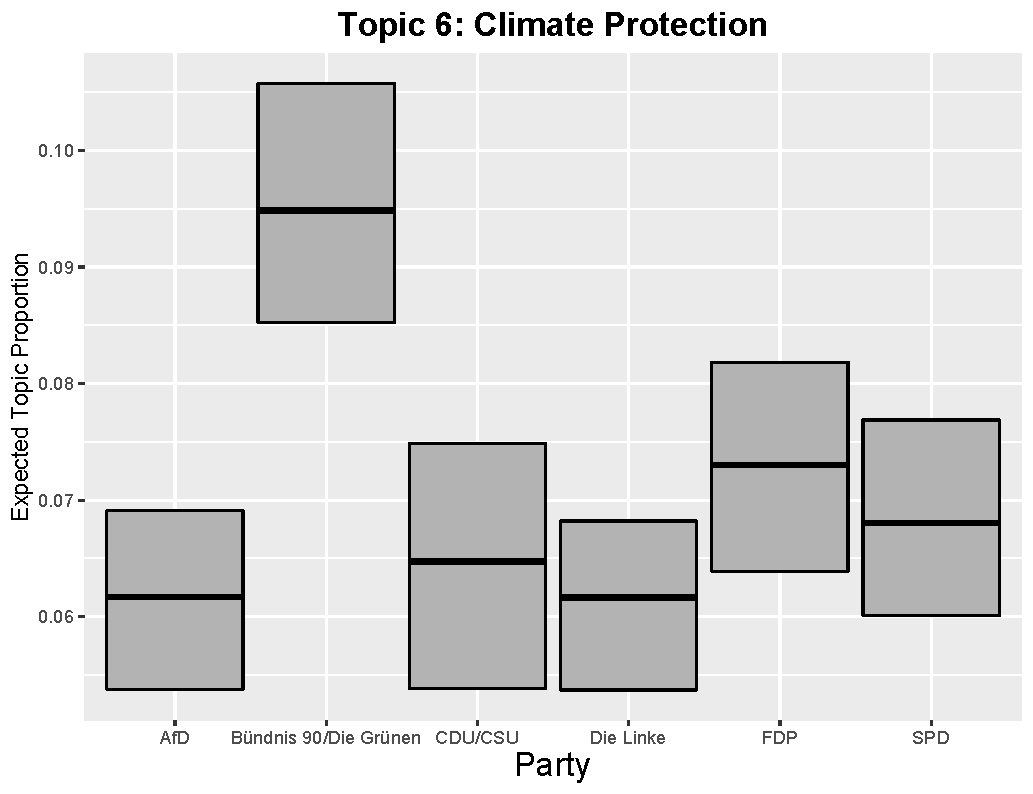
\includegraphics[width=\linewidth]{../plots/appendix/4_6/beta_t6_cat_ctm.pdf}
  \end{subfigure}
  \caption{blabla}
  \label{fig:beta_t46_cat_ctm}
\end{figure}

\begin{figure}[h!]
  \centering
  \captionsetup{justification=centering,margin=2cm}
  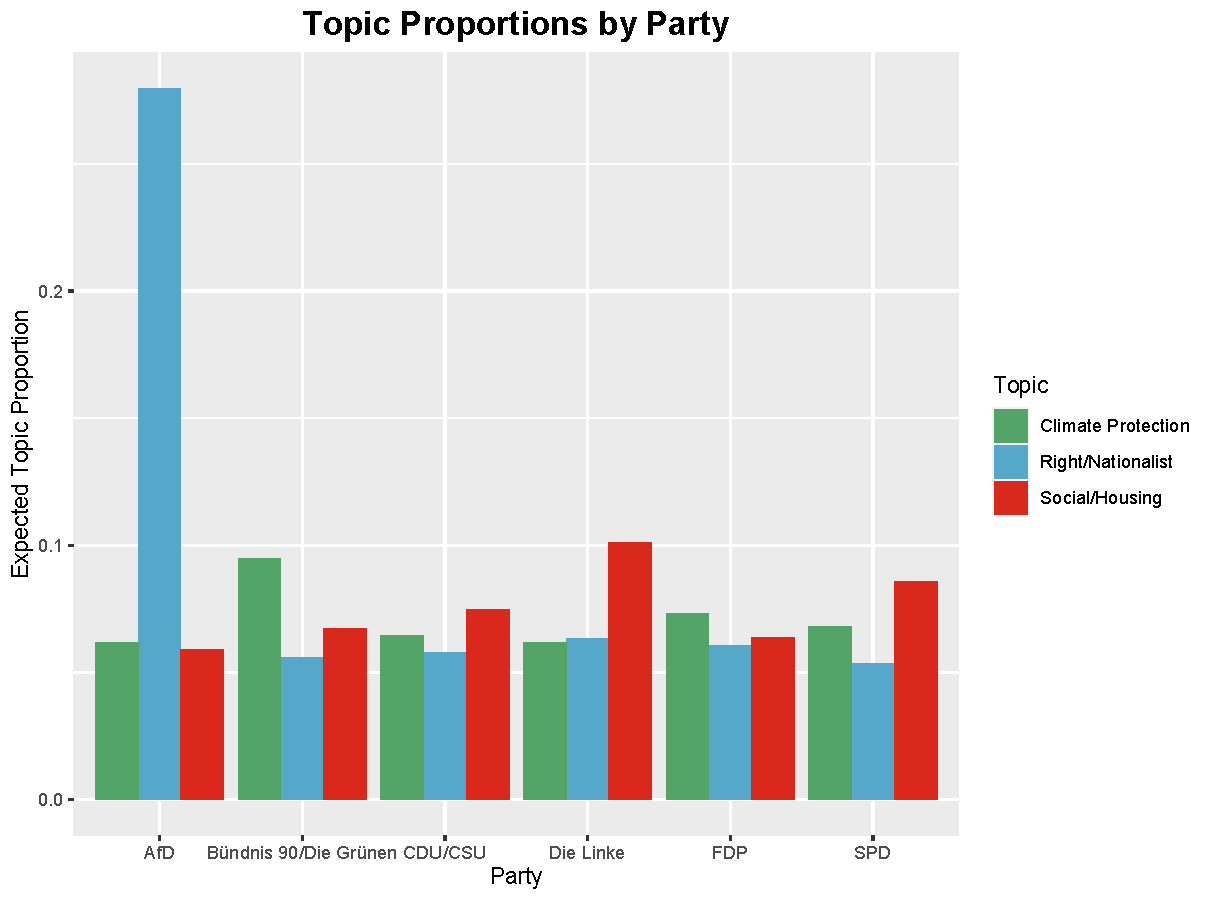
\includegraphics[scale = 0.5]{../plots/appendix/4_6/beta_t146_cat_ctm.pdf}
  \caption{Topical prevalence by political party for topics 1, 2, and 3.}
  \label{fig:beta_t146_cat_ctm}
\end{figure}
\clearpage

\bibliography{./kapitel/bibliography}
\bibliographystyle{plainnat}

\end{document}
